\input{./econtexRoot}\input{\econtexRoot/econtexPaths}\documentclass[titlepage]{\econtex}\providecommand{\texname}{BufferStockTheory}


\providecommand{\EqDir}{Equations}
\providecommand{\FigDir}{Figures}
\providecommand{\CodeDir}{Code}
\providecommand{\CalibrationDir}{Calibration}
\providecommand{\TableDir}{Tables}
\providecommand{\ApndxDir}{Appendices}

\usepackage{subfiles}

\providecommand{\onlyinsubfile}{}
\providecommand{\notinsubfile}{}
\renewcommand{\onlyinsubfile}[1]{}
\renewcommand{\notinsubfile}[1]{#1} 


\usepackage{\econtexSetup}\usepackage{\econtexShortcuts}\usepackage{makecell} 
\input{./econtexRoot}\input{\econtexRoot/econtexPaths}\documentclass[titlepage]{\econtex}\providecommand{\texname}{BufferStockTheory}


\providecommand{\EqDir}{Equations}
\providecommand{\FigDir}{Figures}
\providecommand{\CodeDir}{Code}
\providecommand{\CalibrationDir}{Calibration}
\providecommand{\TableDir}{Tables}
\providecommand{\ApndxDir}{Appendices}

\usepackage{subfiles}

\providecommand{\onlyinsubfile}{}
\providecommand{\notinsubfile}{}
\renewcommand{\onlyinsubfile}[1]{}
\renewcommand{\notinsubfile}[1]{#1} 


\usepackage{\econtexSetup}\usepackage{\econtexShortcuts}\usepackage{makecell} 
\input{./econtexRoot}\input{\econtexRoot/econtexPaths}\documentclass[titlepage]{\econtex}\providecommand{\texname}{BufferStockTheory}


\providecommand{\EqDir}{Equations}
\providecommand{\FigDir}{Figures}
\providecommand{\CodeDir}{Code}
\providecommand{\CalibrationDir}{Calibration}
\providecommand{\TableDir}{Tables}
\providecommand{\ApndxDir}{Appendices}

\usepackage{subfiles}

\providecommand{\onlyinsubfile}{}
\providecommand{\notinsubfile}{}
\renewcommand{\onlyinsubfile}[1]{}
\renewcommand{\notinsubfile}[1]{#1} 


\usepackage{\econtexSetup}\usepackage{\econtexShortcuts}\usepackage{makecell} 
\input{./econtexRoot}\input{\econtexRoot/econtexPaths}\documentclass[titlepage]{\econtex}\providecommand{\texname}{BufferStockTheory}


\providecommand{\EqDir}{Equations}
\providecommand{\FigDir}{Figures}
\providecommand{\CodeDir}{Code}
\providecommand{\CalibrationDir}{Calibration}
\providecommand{\TableDir}{Tables}
\providecommand{\ApndxDir}{Appendices}

\usepackage{subfiles}

\providecommand{\onlyinsubfile}{}
\providecommand{\notinsubfile}{}
\renewcommand{\onlyinsubfile}[1]{}
\renewcommand{\notinsubfile}[1]{#1} 


\usepackage{\econtexSetup}\usepackage{\econtexShortcuts}\usepackage{makecell} 
\input{\econtexRoot/BufferStockTheory.sty}

\provideboolean{Shorter}
\setboolean{Shorter}{true}
\setboolean{Shorter}{false}
\providecommand{\ShorterYN}{\ifthenelse{\boolean{Shorter}}}
\usepackage{rotating}\usepackage{subfigure}


\hypersetup{pdfauthor={William Du <wdu9@jhu.edu>},
            pdftitle={Theoretical Foundations of Buffer Stock Saving},
            pdfkeywords={Precautionary saving, buffer-stock saving, consumption, marginal propensity to consume, permanent income hypothesis},
            pdfcreator = {wdu9@jhu.edu}
}

\begin{document}\bibliographystyle{\econtexBibStyle}
\renewcommand{\onlyinsubfile}[1]{}\renewcommand{\notinsubfile}[1]{#1} 

\hfill{\tiny \texname.tex, \today}

\begin{verbatimwrite}{\texname.title}
Theoretical Foundations of Buffer Stock Saving
\end{verbatimwrite}


\title{Distribution of Wealth and Monetary Policy}

\author{William Du\authNum}

\keywords{Precautionary saving, Heterogeneous Agents, Monetary Policy, permanent income hypothesis}




\maketitle 


\hypertarget{abstract}{}
\begin{abstract}
  This paper develops a heterogenous agent new keynesian model featuring a buffer stock income process, both sticky wages and prices and heterogeneity in discount factors to generate high aggregate MPC.
\end{abstract}


\begin{authorsinfo}
\name{Contact: \href{mailto:wdu9@jhu.edu}{\texttt{wdu9@jhu.edu}}}
\end{authorsinfo}

\thanks{Thanks to }

\titlepagefinish


\newtheorem{defn}{Definition}
\newtheorem{theorem}{Theorem}

\hypertarget{Introduction}{}
\section{Introduction}

\label{sec:intro}


Write here for intro



\hypertarget{The-Model}{}
\section{The Model}

\subsection{Households}
\label{subsec:Households} 

There is a continuum of households of mass 1 distributed on the unit
interval and indexed by $i$. Households are ex-ante heterogeneous in their discount factors and subject to idiosyncratic income shocks.  Each household faces the following problem:

\begin{verbatimwrite}{\EqDir/supfn.tex}
\begin{eqnarray}
  \label{eq:supfn}
  \max_{\{\cLevBF_{it+s}\}_{s=0}^{\infty}} \mathrm{E_{t}}\left[\sum_{s=0}^{\infty} (\not D \beta_{i})^{t+s} U\left(  \cLevBF_{i t+s}, n_{i t+s}\right)\right]
\end{eqnarray}
\end{verbatimwrite}
\input{\EqDir/supfn.tex} 

subject to 
\begin{align*}
\aLevBF_{it}     &= \mLevBF_{it} - \cLevBF_{it}   \label{eq:DBCparts} \\
\aLevBF_{it} +\cLevBF_{it}    &= \mathbf{z}_{it} +   (1 + r^{a}_{t} ) \aLevBF_{it-1}   \\ 
\aLevBF_{it}  &\geq 0 \\
\end{align*}

where
$U\left(\cLevBF_{i t}, n_{i t}\right) = \frac{\cLevBF_{i t}^{1-\rho}}{1 -\rho} - \varphi \pLevBF_{it} \frac{n_{it}^{1+v}}{1+v}$  and $\beta_{i}$ is the discount factor of household $i$. $\mLevBF_{it}$ \ denotes household $i$'s market resources at time $t$ to be expended on consumption or invested at a mutual fund. $\cLevBF_{it}$ is the level of consumption of household $i$ at time $t$ and  $ \aLevBF_{it}$ is the value of household $i$'s shares at the mutual during period $t$ where the mutual fund's return is $r_{t+1}^{a}$.  $\mLevBF_{it}$ is determined by labor income,  $\mathbf{z}_{it}$, and the gross return on assets from the last period, $(1+r_{t}^{a}) \aLevBF_{it-1} $. $\not D$ is the probability of death. Death is included in our model to ensure permanent income, $\pLevBF$, and thus wealth, has a limiting distribution.   Labor supply of household $i$ at time $t$ is denoted by $n_{it}$.  Given the formulation of sticky wages described in section 2.4, labor supply is an aggregate state variable and therefore consumption serves as the sole control variable in the dynamic problem.  \\





\begin{align*}
\mathbf{z}_{it} &= \pLevBF_{it}\tShkAll_{it} \\
\pLevBF_{it+1} &=\pLevBF_{it} \pShk_{it+1} \\
\end{align*}


Labor income is subject to permanent and transitory idiosyncratic shocks. In particular, household $i$'s labor income is composed of a permanent component, $\pLevBF_{it} $ indicating the level of permanent income and a transitory component, $\tShkAll_{it} $, indicating the transitory income shock received by household $i$ at time $t$. $\pLevBF_{it} $ is subject to permanent income shocks $\pShk_{it+1}$ where $\pShk_{it}$ is iid mean one lognormal with standard deviation $\sigma_\pShk$, $\forall t$ . \\



The transitory component follows   \\
\begin{verbatimwrite}{\EqDir/tShkDef}
$$
\tShkAll _{it}=
\begin{cases}
 u \phantom{_{t+1}/\pNotZero} & \text{with probability $\mho $} \\
 \tShkEmp_{it} (1-\tau_{t})\int_{0}^{1} w_{gt}n_{igt} \, dg      & \text{with probability $1 - \mho  $} 
\end{cases} \label{eq:tShkDef}
$$
\end{verbatimwrite}
\input{\EqDir/tShkDef.tex}\\
where u is unemployment benefits, $\tau_{t}$ is the tax rate , $w_{gt}$ is the real wage for labor type $g$ at time t, $ n_{igt}$ is the labor supply for labor type $g$ and $\tShkEmp_{t}$ is an iid mean-one lognormal with standard deviation $\sigma_{\tShkEmp}$.  The probability of receiving an unemployment shock in a given period where households forego their after-tax labor income and receive unemployment benefits instead is denoted by $\mho$.  \\ \\

Given the formulation of sticky wages described in section 2.4, the transitory component simplifies to \\

\begin{equation}
\tShkAll _{it}=
\begin{cases}
 u \phantom{_{t+1}/\pNotZero} & \text{with probability $\mho $} \\
 \tShkEmp_{it} (1-\tau_{t})\frac{w_{t}N_{t}}{(1-\mho)}      & \text{with probability $1 - \mho  $} 
\end{cases} \label{eq:tShkDef}
\end{equation} 

where $w_{t}$ is the real wage and $N_{t}$  is labor supply.

For details on the derivation, see Appendix.\\ \\


\begin{comment}
Combining the transition equations, the recursive nature of
the problem allows us to rewrite it more compactly in Bellman equation form,
\begin{eqnarray*}
\VFunc_{t}(\mLevBF_{t},\pLevBF_{t}) & = & \max_{\cLevBF_{t}}~\left\{\util(\cLevBF_{t})+\DiscFac \Ex_{t}\left[ \VFunc_{t+1}((\mLevBF_{t}-\cLevBF_{t})\Rfree+ \pLevBF_{t+1}\tShkAll_{t+1},\pLevBF_{t} \PGro  \pShk_{t+1})\right]\right\}
.
\end{eqnarray*}
\end{comment} 

\hypertarget{Financial Intermediary}{}
\subsection{Financial Intermediary}

\label{subsec:Financial Intermediary}

The financial intermediary in our model performs a mutual fund activity where it  collects assets from households and invests them into government bonds $B_{t}$, stocks $v_{jt}$, and nominal reserves at the central bank $M_{t}$.\\ 

In particular, at the end of period $t$, the assets collected from households $A_{t}$ must be invested into shares $\mathit{v}_{jt}$ of firm $j$ at price  $q^{s}_{jt}$ , government bonds $B_{t}$ at price $q^{b}_{t}$ and nominal reserves $M_{t}$. 

\begin{equation} A_{t} = \frac{M_{t}}{P_{t}} +q^{b}_{t} B_{t} + \int_{0}^{1} q^{s}_{jt}\mathit{v}_{jt}\,dj \end{equation}

where $A_{t} $ is the dollar value of the mutual fund's assets at the end of period $t$ and $ \mathit{v}_{jt}$ is the portfolio share of firm $j$ stocks with $\int_{0}^{1} \mathit{v}_{jt}\,dj =1$.  \\

The mutual fund's return in the next period is then 

$$(1+r^{a}_{t+1})  = \frac{  B_{t} + \int_{0}^{1} (q^{s}_{jt+1}+ D_{jt+1})\mathit{v}_{jt} \, dj +(1+i_{t}) \frac{M_{t}}{P_{t+1}}}{A_{t}}$$\\ 

where  $D_{jt+1}$ are dividends of firm $j$ and $i_{t}$ is the nominal interest rate  on nominal reserves. \\ \\

The mutual fund is risk neutral and looks to maximize its expected return 


$$\max_{\{B_{t}, M_{t} , \mathit{v}_{jt} \}} \mathrm{E}_{t}\left[1+r^{a}_{t+1} \right] = \mathrm{E}\left[ \frac{ B_{t} + \int_{0}^{1} (q^{s}_{jt+1}+ D_{jt+1})\mathit{v}_{jt} \, dj +(1+i_{t}) \frac{M_{t}}{P_{t+1}}}{\frac{M_{t}}{P_{t}} +q^{b}_{t} B_{t} + \int_{0}^{1} q^{s}_{jt}\mathit{v}_{jt}\,dj} \right]$$ \\

 
The first order conditions lead to the no arbitrage equations:

\begin{equation} \mathrm{E}_{t}\left[1+r^{a}_{t+1}\right]= \frac{1}{q^{b}_{t}}  =\frac{\mathrm{E}_{t}\left[q^{s}_{jt+1} + D_{jt+1} \right]}{q^{s}_{jt}} = (1+i_{t}) \mathrm{E}_{t}\left[\frac{P_{t}}{P_{t+1}}\right] \equiv 1 +r_{t} \end{equation}

where $r_{t}$ is defined to be the real interest rate in period $t$. 
In equilibrium ,we will assume $M_{t} =0$ \\ \\

\hypertarget{Goods Market}{}
\subsection{Goods Market}

There is a continuum of  monopolistically competitive intermediate good producers indexed by $j \in [0,1]$ who produce intermediate goods $Y_{jt}$ to be sold to a final good producer at price $P_{jt}$. Using intermediate goods $Y_{jt}$ for $j \in [0,1]$, the  final good producer produces a final good $Y_{t}$ to be sold to households at price $P_{t}$.  \\ 


\hypertarget{Final Good Producer}{}
\subsubsection{Final Good Producer}

A perfectly competitive final good producer purchases intermediate goods $Y_{jt}$ from intermediate good producers at price $P_{jt}$ and produces a final good $Y_{t}$ according to a CES production Function. 

$$ Y_{t} = \left(\int_{0}^{1} Y_{jt}^{\frac{\epsilon_{p}-1}{\epsilon_{p}}}\, dj\right)^{\frac{\epsilon_{p}}{\epsilon_{p}-1}}$$ \\

where $\epsilon_{p}$ is the elasticity of substitution. \\ 

Given $P_{jt}$ , the price of intermediate good $j$ ,  the final good producer maximizes his profit

$$ \max_{Y_{jt}} P_{t} \left(\int_{0}^{1} Y_{jt}^{\frac{\epsilon_{p}-1}{\epsilon_{p}}}\, dj\right)^{\frac{\epsilon_{p}}{\epsilon_{p}-1}} - \int_{0}^{1} P_{jt} Y_{jt} ,\ dj $$ \\


The first order condition leads to demand for good $j$

\begin{equation} Y_{jt} = \left(\frac {P_{jt}}{P_{t}}\right)^{- \epsilon_{p}} Y_{t}\end{equation} \\

and the price index

\begin{equation} P_{t} = \left(\int_{0}^{1} P_{jt}^{1-\epsilon_{p}}\,dj \right )^{\frac{1}{1-\epsilon_{p}}} \end{equation}


\hypertarget{Intermediate Good Producer}{}
\subsubsection{Intermediate Good Producer}

Intermediate goods producers  employ labor and produce according to a Cobb Douglas Production function.  

$$Y_{jt} =  Z_{t}  N_{jt}$$ 

where $log(Z_{t}) = \rho_{Z} log( Z_{t-1}) + \epsilon_{Z}$ \\ \\


Prices are sticky a la Calvo where each period intermediate good producers may reset their price with probability $ 1 -\lambda_{p}$ . Following Auclert et al 2020., each intermediate firm $j$ chooses $P_{jt}$ to maximize its dividend $D_{jt}$ and  stock price $q^{s}_{jt} $ \\ 
 
 $$\max_{\{P_{jt}\}} \overbrace{\frac{(P_{jt} - MC_{t})Y_{jt}}{P_{t}}}^{=D_{jt}} + q^{s}_{jt}\left(P_{jt}\right) $$ \\
 
where  $q^{s}_{jt}\left(P_{jt}\right) = \frac{\mathrm{E}_{t}\left[q^{s}_{jt+1} +D_{jt+1}\left(P_{jt}\right)\right]}{1+r_{t}}$ \\ \\

The problem above can be restated as 
 
 $$\max_{\{P_{jt}\}} \mathrm{E}_{t}\left[\sum_{s=0}^{\infty} (\lambda_{P}) ^{s} M_{t,t+s} \left[ \frac{(P_{jt} - MC_{t+s})Y_{jt+s}}{P_{t+s}}\right]\right]$$
 
subject to $$Y_{jt} = \left(\frac {P_{jt}}{P_{t}}\right)^{- \epsilon_{p}} Y_{t}$$
 
where $M_{t, t+s} = \prod_{k=t}^{t+s-1} \frac{1}{1+r_{k}}$ is the stochastic discount factor and $MC_{t} = \frac{W_{t}}{A_{t}}$ is the marginal cost of firm $j$.  \\ \\


This problem leads to the Phillips Curve in our model \\ 

\begin{equation} \pi_{t}^{p} = \frac{\mathrm{E}_{t}[\pi_{t+1}^{p}]}{1+r^{*}} + \lambda (\mu_{t}^{p} -\mu^{p}) \end{equation}

where $r^{*}$ is the natural rate of interest in the steady state, $\lambda = \frac{(1-\lambda_{p})(1-\frac{\lambda_{p}}{1+r^{*}})}{\lambda_{p}}$,  $ \mu_{t}^{p} = log(P_{t}) - log(W_{t}) + log(Z_{t})$ and $\mu^{p} = \frac{\epsilon_{p}}{1-\epsilon_{p}}$ \\ \\



\hypertarget{Labor Market}{}
\subsection{Labor Market}

Given the probability of receiving an unemployment shock is $\mho$, we assume, without loss of generality, households $i \in [\mho,1]$ are `employed'  with positive labor supply and households $i \in [0, \mho]$  are `unemployed' and provide no labor. 

$$
n _{it}=
\begin{cases}
 k  & \text{if  $i \in [\mho, 1]$} \\
 0      & \text{if  $i \in [0, \mho]$} 
\end{cases} 
$$

where $k>0$. \\

There is a continuum of monopolistically competitive labor unions indexed by $g \in [0,1]$ that collects labor $n_{igt} > 0$ from employed households $i \in [\mho,1]$ . Labor supply of household $i \in [\mho,1]$ is then

$$n_{it} = \int_{0}^{1} n_{igt}\,dg$$ \\

Following Auclert et al 2020., we assume each labor union $g$ demands the same level  of labor supply from each household. Denote $n_{gt}$ the level of labor demanded from each household by labor union $g$ at time $t$, that is,  assume  $n_{igt} =\mathit{n}_{gt}$. This assumption will imply labor income heterogeneity to be solely the consequence of  permanent and transitory income shocks.
The total level of labor collected from employed households  by labor union $g$  is then 

$$  (1-\mho) \mathit{n}_{gt} = \int_{\mho}^{1} n_{igt}\,di $$ \\

Each period $t$, labor unions sell their labor collected from households to a competitive labor packer who demands labor $N_{gt}$ at price $W_{gt}$ from union $g$ . 

Thus, in equilibrium, $$  N_{gt} = (1-\mho) \mathit{n}_{gt} = \int_{\mho}^{1} n_{igt}\,di $$  \\


\hypertarget{Competitive Labor Packer}{}
\subsubsection{Competitive Labor Packer}



A perfectly competitive labor packer purchases labor $N_{gt}$ from labor unions $g \in [0,1]$ and produces $N_{t}$ using constant elasticity of substitution technology be sold to firms at price $W_{t}$

 
$$ N_{t} = \left(\int_{0}^{1} N_{gt}^{\frac{\epsilon_{w}-1}{\epsilon_{w}}}\,dg\right)^{\frac{\epsilon_{w}}{\epsilon_{w}-1}}$$ \\

The labor packer's maximizes its profit with respect the menu of wages $W_{gt}$ for $ g \in  [0,1]$

$$ \max_{n_{jgt}} W_{t} \left(\int_{0}^{1} N_{jgt}^{\frac{\epsilon_{w}-1}{\epsilon_{w}}} \, dg \right)^ {\frac{\epsilon_{w}}{\epsilon_{w}-1}} - \int_{0}^{1} W_{gt}N_{jgt}\, dj $$ \\


The first order condition leads to the labor packer's demand for labor type $g$

$$ N_{gt} = \left(\frac{W_{gt}}{W_{t}}\right)^{-\epsilon_{w}} N_{t} $$

and wage index follows
$$ W_{t} = \left(\int_{0}^{1} W_{gt}^{1-\epsilon_{w}}\,dg\right)^{\frac{1}{1-\epsilon_{w}}}$$ \\




\hypertarget{Labor Unions}{}
\subsubsection{Labor Unions}

Labor Union $g$  sets its wage to maximize the expected aggregate lifetime utility of all employed households. Wages are sticky a la Calvo where unions may adjust its wage with probability $\lambda_{w}$. 

$$ \max_{\{W_{gt}\}} \mathrm{E_{t}}\left[\sum_{s=0}^{\infty} (\bar{\beta} \not D \lambda_{w})^{s} \int_{\mho}^{1}  U\left (c_{it+s}(W_{gt+s}), n_{i t+s}) \, di \right)\right] $$

where $\bar{\beta} = \int_{\mho}^{1} \beta_{i} \, di$ \\

subject to the following three constraints $$ N_{gt} = \left(\frac{W_{gt}}{W_{t}}\right)^{-\epsilon_{w}} N_{t} $$
$$  N_{gt} = (1-\mho) \mathit{n}_{gt} = \int_{\mho}^{1} n_{igt}\,di $$ 

$$ W_{t} = \left(\int_{0}^{1} W_{gt}^{1-\epsilon_{w}}\,dg\right)^{\frac{1}{1-\epsilon_{w}}}$$ \\



The wage Phillips Curve follows from the first order condition


$$ \pi_{t}^{w} =   \bar{\beta} \not D  \mathrm{E}_{t} \left[ \pi_{t+1}^{w}\right] + \frac{(1-\lambda_{w})}{\lambda_{w}} (1- \bar{\beta} \not D \lambda_{w}) (\mu^{w} - \mu_{t}^{w})$$ \\

where $\mu^{w}$ is the optimal wage markup and the wage markup is defined as \\ 

$\mu_{t}^{w} = log\left( \frac{W_{t}}{P_{t}}\right)  - log\left(1 -\tau \right) - mrs_{t}$ \\


$ mrs_{t} = log \left(- \frac{\int_{0}^{1}   U_{n} \left(c_{i t}, n_{i t} \right) \ d i  }{\int_{0}^{1}  p_{it} \theta_{it} U_{c} \left(c_{i t}, n_{i t} \right) \  di } \right) \\ \\ $


\hypertarget{Government Policy}{}
\subsection{Government Policy}



\hypertarget{Fiscal Policy}{}
\subsubsection{Fiscal Policy}

The government funds its purchases and unemployment insurance payments by issuing debt and taxing labor income. In particular, it follows 

$$ B_{t-1} + G + \mathit{u} \mho =   q^{b}_{t} B_{t} +  \tau \int_{0}^{1} \int_{0}^{1} w_{igt} n_{igt} \, dg \, di$$ \\

which simplifies to 

$$ B_{t-1} + G + \mathit{u} \mho =   q^{b}_{t} B_{t} +  \tau w_{t}N_{t}$$  \\


where $G $ is government expenditures. \\



\hypertarget{Monetary Policy}{}
\subsubsection{Monetary Policy}


The central bank follows the taylor rule: 

$$i_{t} = r^{*} +\phi_{\pi} \pi^{p}_{t} + \phi_{y} (Y_{t} - Y_{ss}) + \epsilon^{m}_{t}$$ \\

where $\phi_{\pi}$ is the Taylor rule coefficient for inflation, $\phi_{y}$ is the Taylor rule coeffficient for output gap,  $r^{*}$ is the steady state interest rate, $Y_{ss}$ is the steady state level of output,  $\epsilon^{m}_{t} = \rho_{v} v_{t-1} +\varepsilon_{t}$ is a monetary policy shock. \\

\hypertarget{Equilibrium}{}
\subsection{Equilibrium}


An equilibrium in this economy is a sequence of: \\

- Policy Functions $\left( c_{it}(m) \right )_{t=0}^{\infty}$ \\

- Value functions $ \left( V_{t}(m) \right)_{t=0}^{\infty}$\\

- Prices $ \left(r_{t},  r^{a}_{t+1}, i_{t}, q^{s}_{t}, q^{b}_{t}, w_{t} , \pi^{p}_{t}, \pi^{w}_{t} \right) _{t=0}^{\infty}$\\

- Aggregates $ \left(C_{t}, Y_{t} , N_{t}, D_{t} , A_{t} , B_{t} \right)_{t=0}^{\infty}$\\

Such that: \\

$ \left(  c_{it}(m)\right)_{t=0}^{\infty}$  solves the household's maximization problem given $  \left( w_{t}, N_{t},  r^{a}_{t} \right)_{t=0}^{\infty}$.\\

The Mutual fund, final goods producer, intermediate goods producers, labor packer, and labor unions maximize their objective function. \\

The government budget constraint holds. \\

The nominal interest rate is set according to the central bank's Taylor rule. \\


Markets clear:

 $$ A_t = q^{b}_{t} B_{t} + q^{s}_{t} =  \int_{0}^{1} \pLevBF_{it}\left( m_{it} - c_{it}(m_{it})\right) \, di $$
 
 $$ Y_t = C_{t} +G $$ \\
 
 where $C_{t} \equiv  \int_{0}^{1} \pLevBF_{it} c_{it}(m_{it})\, di $ \\


\hypertarget{Computational Methodology}{}
\section{Computation Methodology}

\hypertarget{Household's Problem}{}
\subsection{Household's Problem}

We solve the household's problem by iterating over the first order condition and applying the endogenous gridpoints method developed by Carroll (2006). The computational efficiency for obtaining the consumption policies is greatly improved by dividing the variables of the household's problem by the level of permanent income $\pLevBF_{it}$, leaving normalized market resources $m_{it}$ as the sole state variable ( See Appendix  A.1).  

\hypertarget{General Equilibrium Steady State}{}
\subsection{General Equilibrium Steady State}

To compute the steady state of the model, we begin with a guess of the mean of the uniformly distributed discount factors to target a predetermined interest rate.  With the steady state consumption policy, we simulate the model forward periods and compute the aggregate level of consumption $ C_{t} =  \int_{0}^{1} \pLevBF_{it} c_{it}(m_{it})\, di$  and the aggregate level of assets $ A_{t} = \int_{0}^{1} \pLevBF_{it} \left( m_{it} -  c_{it}(m_{it}) \right)$ for the terminal period. If either the goods or asset market does not clear given the computed aggregate levels of consumption and assets,  we input a new guess of the mean of the discount factors and solve and simulate the model again. We repeat this process until the goods and asset markets clear.  


\hypertarget{General Equilibrium Impulse Responses}{}
\subsection{General Equilibrium Impulse Responses}

To compute the impulse responses of the model, we follow the sequence space jacobian method of Auclert et al. (2021). In particular, we define the model as a system of equations in sequence space and then linearize the system around the steady state to solve for the impulse responses to a perfect foresight ``MIT shock'', that is, an unanticipated shock whose subsequent path is known to all agents.  In a linearized system to first order, aggregate certainty equivalence holds (Simon 1956, Theil 1957),  and therefore the perfect foresight responses to an unexpected shock are the same responses to the shocks of the full stochastic model. For further computational details, see Appendix A.2 . 






\hypertarget{Calibration}{}
\section{Calibration}

\input{\TableDir/Calibration.tex}

Each period in our model represents one quarter of a year. Calibration of household parameters are presented in table 1 while calibration of economy parameters can be found in table 2. There are five discount factors distributed uniformly among agents in the economy with a mean of .9773 and spread of .0049. The discount factors were adjusted to target a 5 percent annual real interest rate. Similarly the disutility of labor is set to .883 to target a labor supply of 1.22 . The target of a 5 percent real interest rate and a labor supply level of 1.22 are completely arbitrary.  The coefficient of risk aversion is set to 2 and the frisch elasticity of labor supply is set to 1/2, in line with Chetty(2012).  The probability of death is set to .99375 to ensure the average working lifespanc of households is $ \frac{1}{(1-.99375)} = 160$ periods, or equivalently, 40 years.  The standard deviations of transitory and permanent shocks follows from CSTW(2017). The rest of household parameters being the unemployment rate, unemployment benefits and the tax rate are all arbitrarily chosen. With regards to the economy calibration, the calvo parameters for price stickiness is set to .85 and the wage stickiness is set .8 both of which lie in the conventional range. The steady price markup is set to 1.012 implying a 1.2 percent markup while the wage markup has been set 1.05 impying a 5 percent wage markup. The taylor rule coefficients have been initially set to zero implying a fixed nominal rate to provide transparency in understanding the impulse responses produced from the model and assess its accuracy without exterior pressures within the model. The taylor coefficients will be modified later when discussing results. The rest of the parameters are arbitrarily chosen. 






\hypertarget{Results}{}
\section{Results}

In this section, we analyze the impulse responses produced from our model for a monetary contraction and a productivity shock.


\hypertarget{Monetary Policy Shock}{}
\subsection{Monetary Policy Shock}

The impulse responses to the monetary policy shock can be found in figure 1. The monetary policy shock is a 100 basis points increase in the nominal rate and follows an AR(1) with a coefficient of .5.  As expected, the rise in the nominal rate leads to a rise in the real interest rate as prices cannot flexibly adjust to clear the goods market. The rise in the real rate leads to a fall in consumption due to the intertemporal substitution channel  causing output to fall as well. This fall in output necessitates a fall in labor demand raising the wage markup $(\frac{W_{t}}{P_{t}} - mrs_{t})$ and thus inducing downward pressure on nominal wages. Downward pressure on nominal wages in turn leads to downward pressure on prices as firm markups rise. Given that prices are stickier than wages and given the downward pressures on both nominal prices and nominal wages, the real wage must fall. The fall in consumption is further amplified from income effects as labor and real wages both fall.  This amplification through the income channel is particularly significant in heterogenous agent new keynesian models as the large aggregate MPC induces consumption to react strongly to the rise in labor and real wages. 


\begin{figure}{Impulse Responses to a Monetary Policy Shock}
  \begin{subfigure}{}
    \centering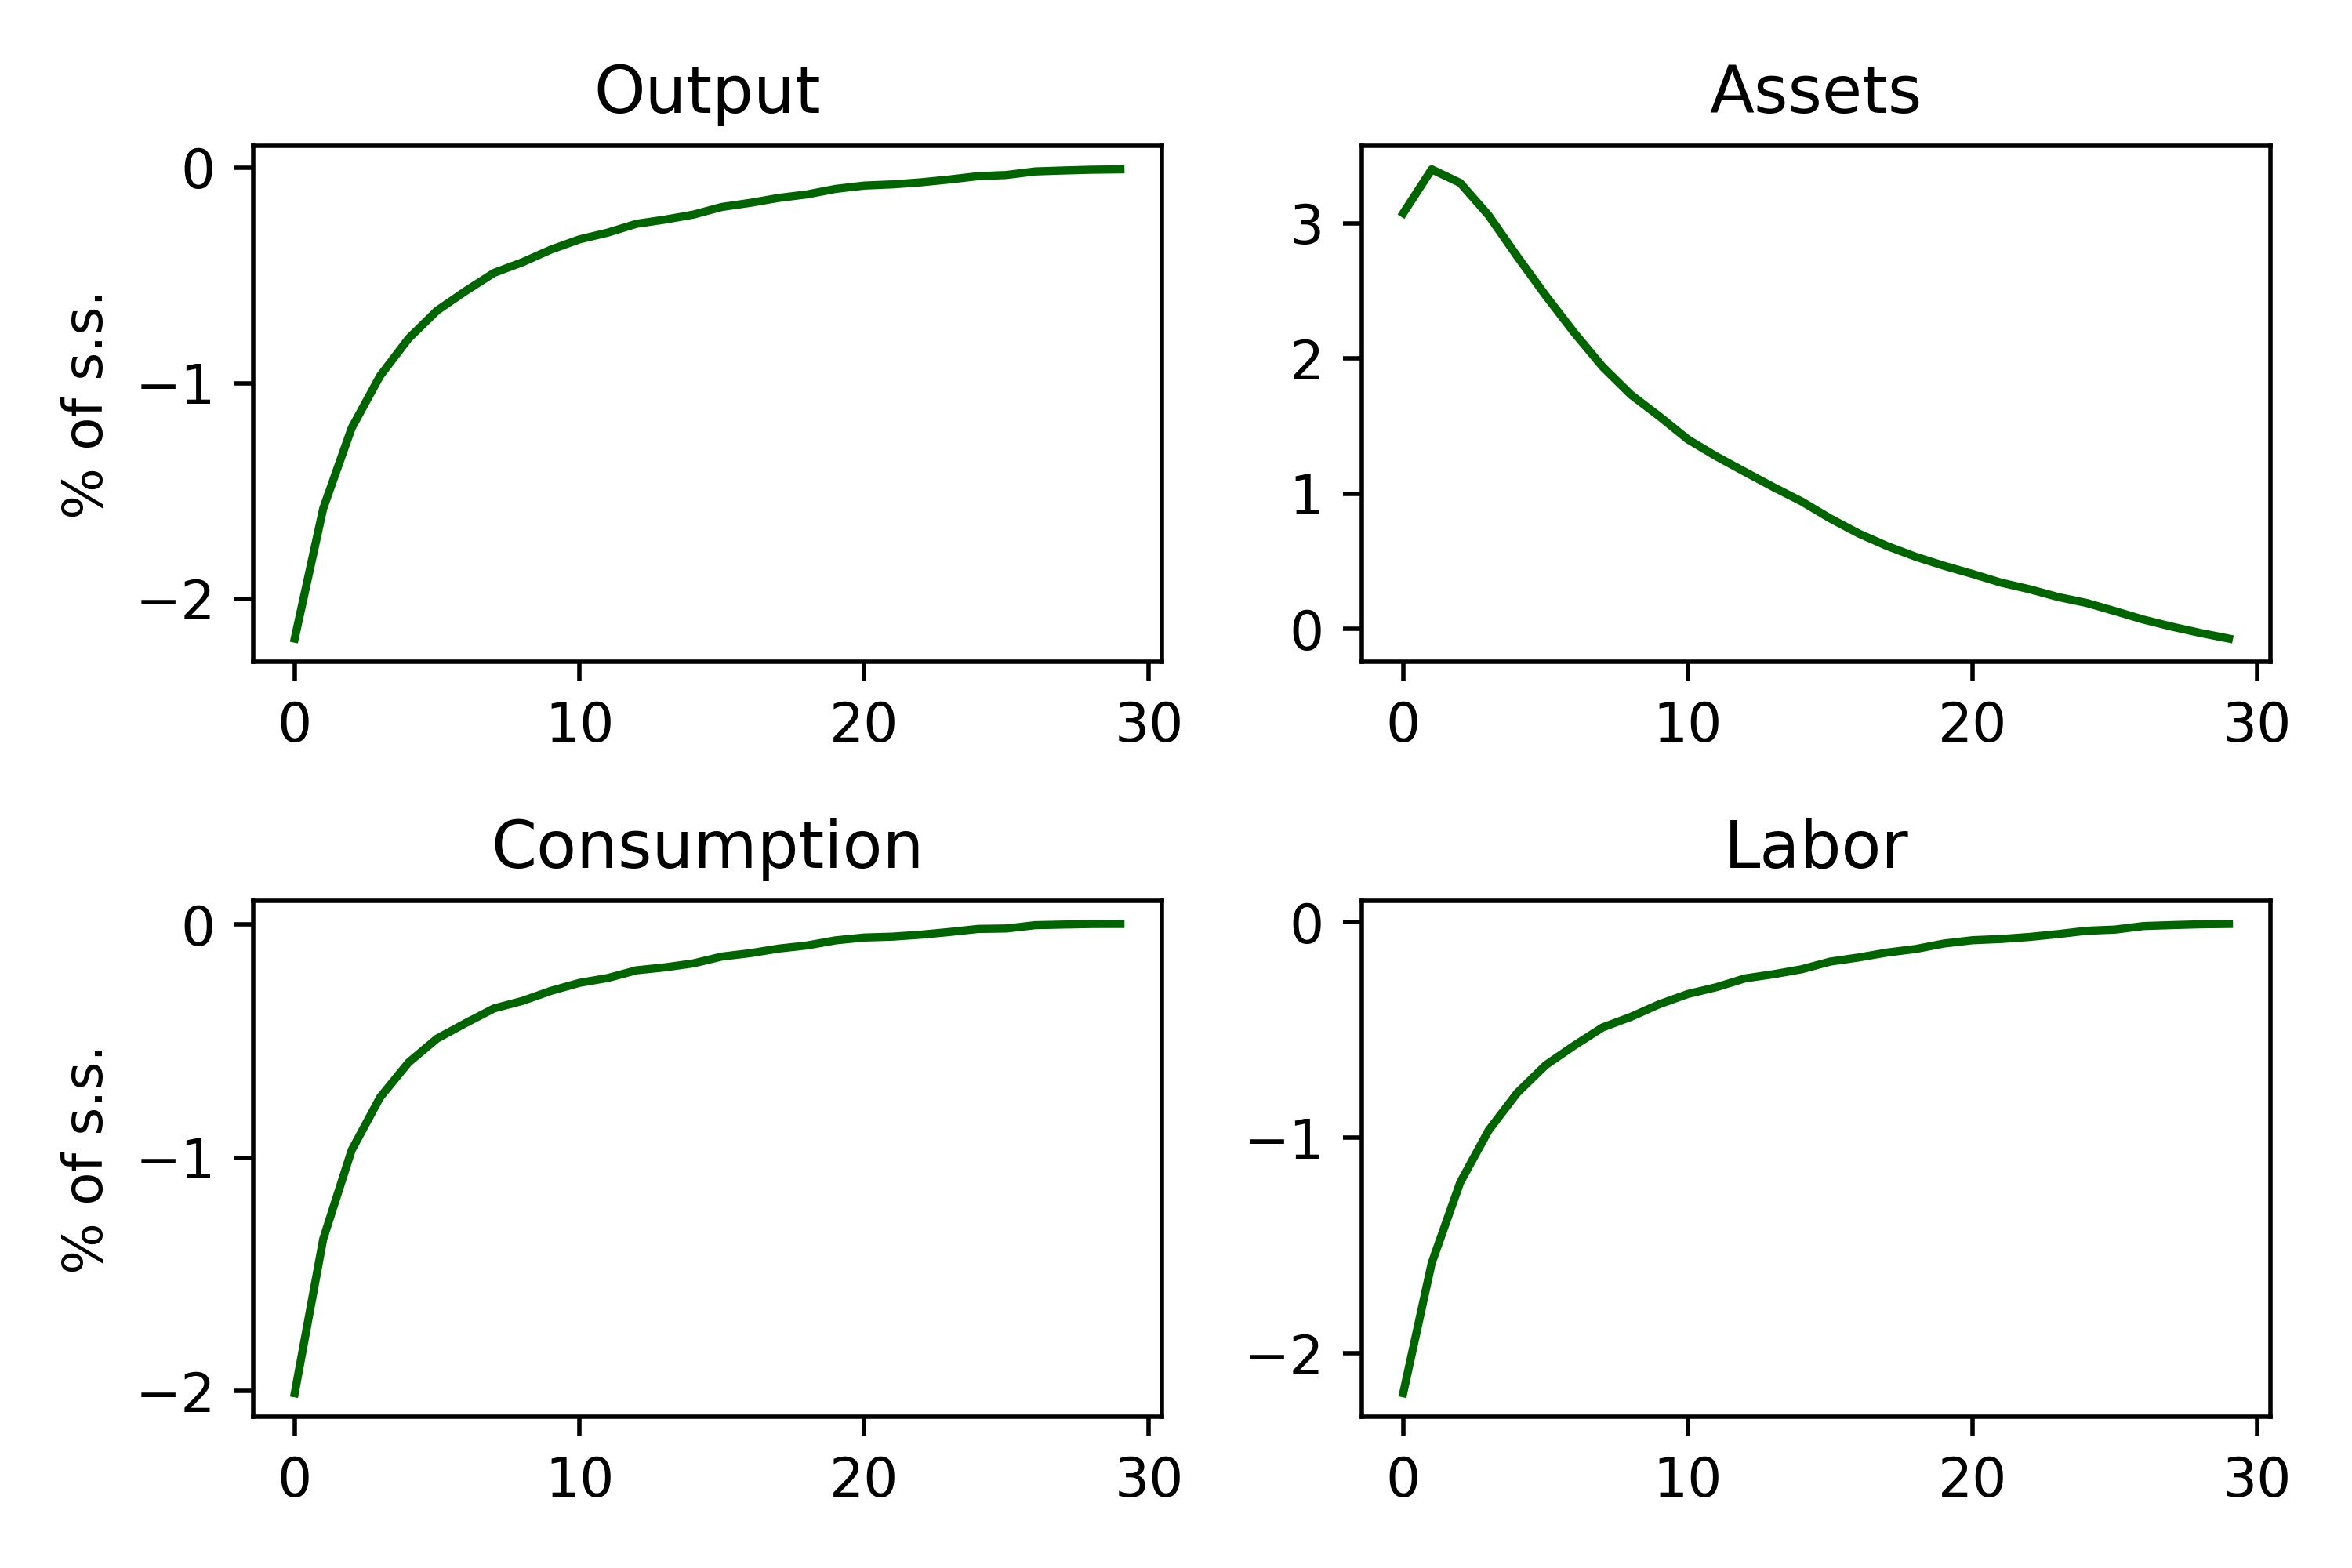
\includegraphics[scale=.35]{\FigDir/GIPRM2}
  \end{subfigure}
  \begin{subfigure}{}
    \centering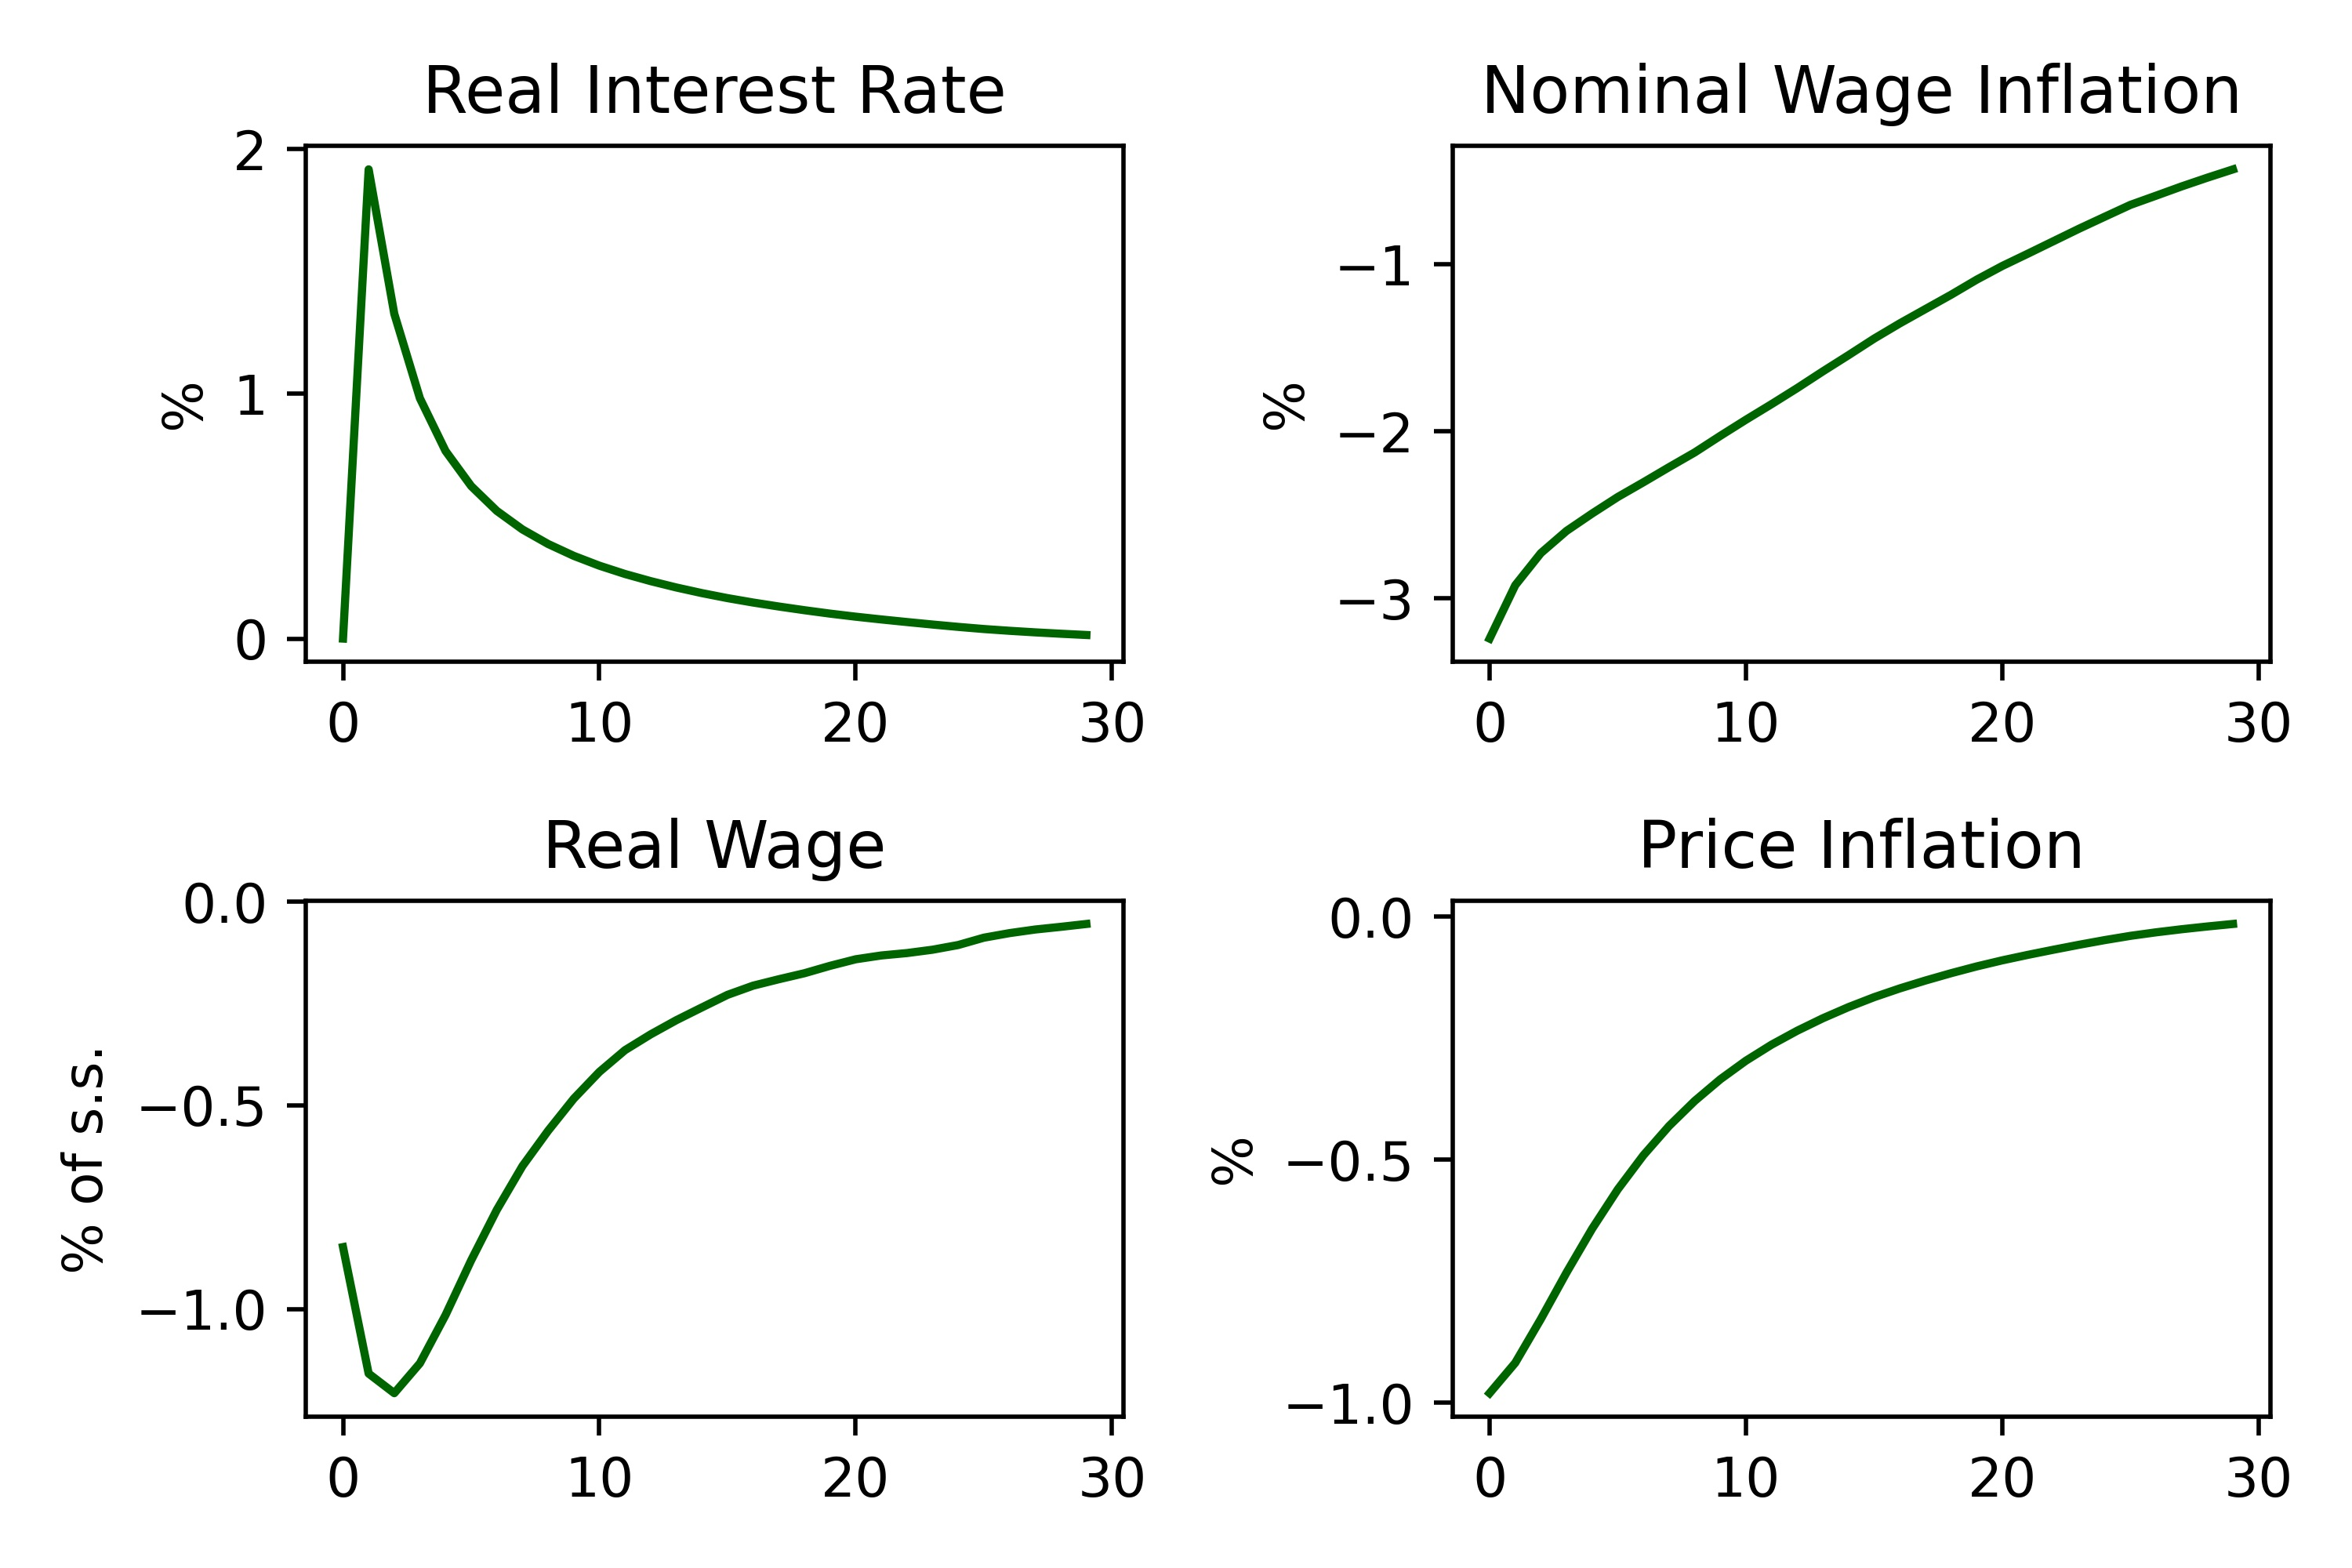
\includegraphics[scale=.35]{\FigDir/GIPRM1}
    \caption{ Impulse Response to One Percent Increase in Nominal Rate}
  \end{subfigure}
\end{figure}


\hypertarget{Productivity Shock}{}
\subsection{Productivity Shock}


The impulse responses to the productivity shock can be found in figure 2. The productivity shock is a 1 percent increase in $Z_{t}$ following an AR(1) with a coefficient of .9. The rise in productivity raises both output and firm markups, inducing downward pressure on prices which inturn induces downward pressure on nominal wages. However, given the goods market must clear, consumption must rise causing upward pressure on the nominal wage since the economy marginal rate of substitution is a function of the average marginal utility of consumption. The net effect will see nominal wages rise leading to upward pressure on prices. The net effect of all these different pressures will see the real wage rise and therefore amplify the consumption response signficantly due to the large aggregate MPC in the model. In addition, to the fixed nominal interest rate, inflation will see the real interest rate fall further amplifying consumption. This amplification of consumption will lead to rises in output and labor due to upward pressure on labor demand.

\begin{figure}{Impulse Responses to a Productivity Shock}
  \begin{subfigure}{}
    \centering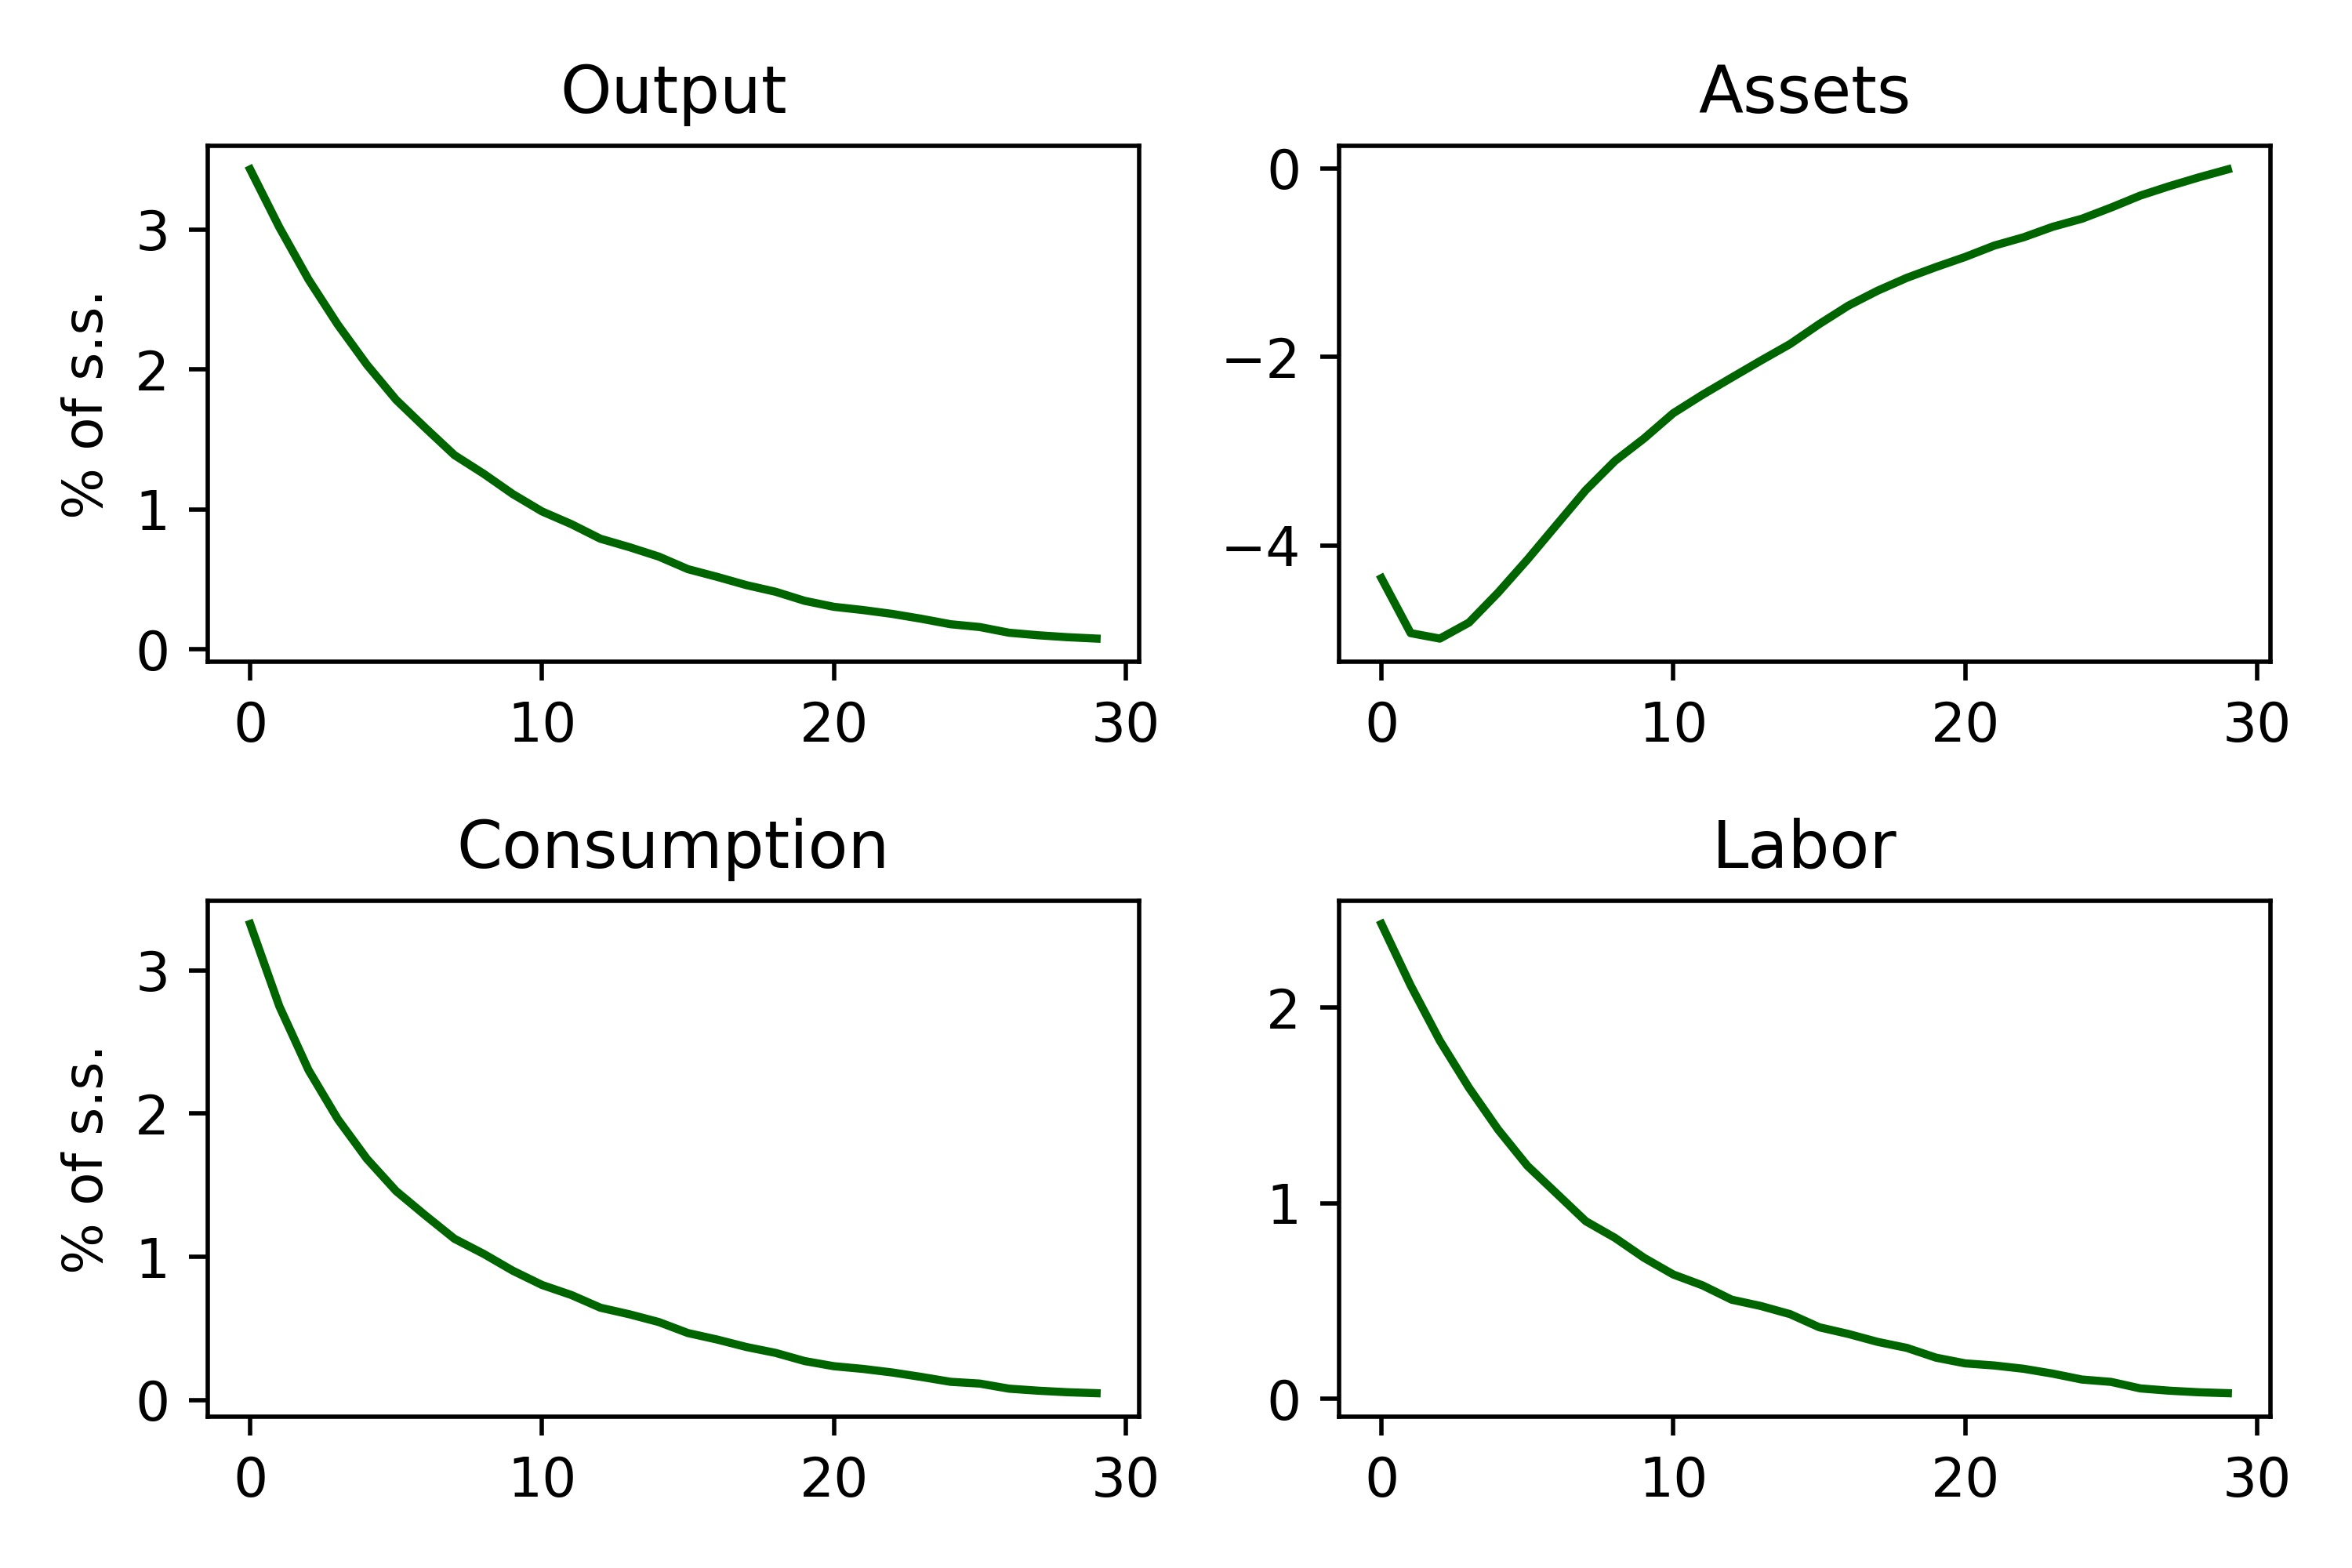
\includegraphics[scale=.35]{\FigDir/GIPRZ2}
  \end{subfigure}
  \begin{subfigure}{}
    \centering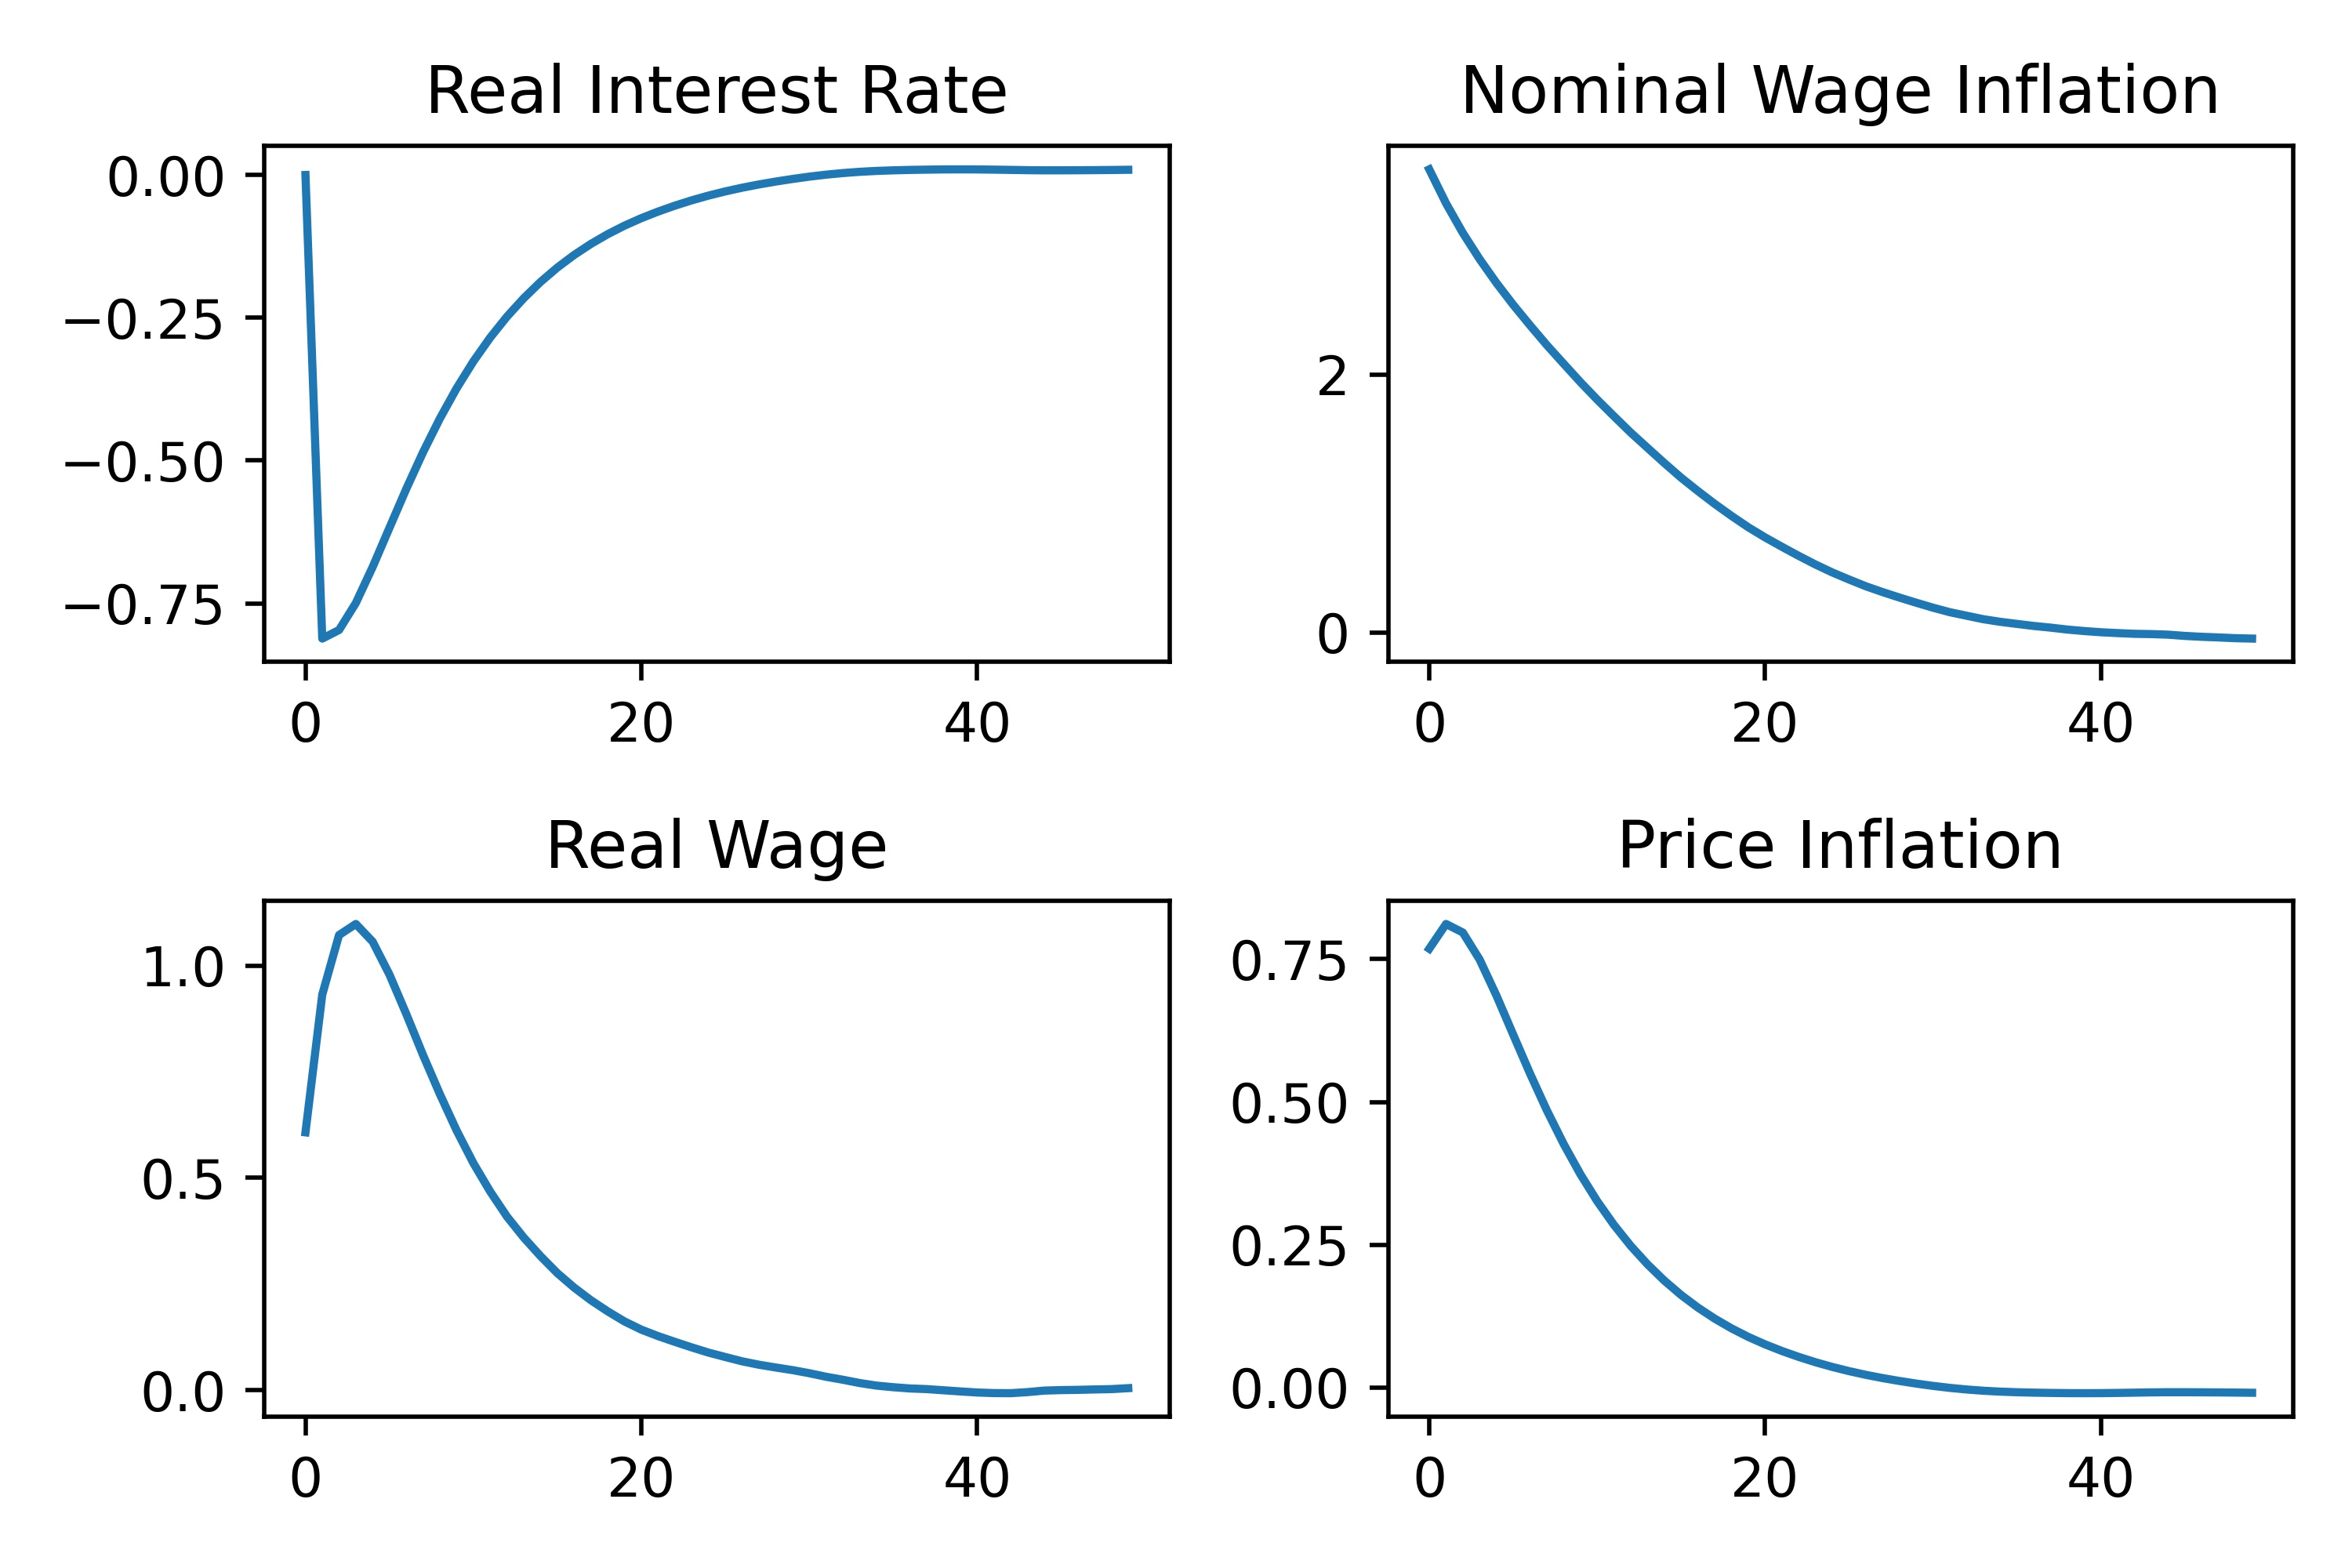
\includegraphics[scale=.35]{\FigDir/GIPRZ1}
    \caption{ Impulse Response to One Percent Increase in $Z_{t}$}
  \end{subfigure}
\end{figure}



\hypertarget{Issues and Extensions}{}
\section{Issues and Extensions}

The most prominent issue I have encountered thus far is determining whether the impulse responses are accurate in regards to the specification of the model. Producing the impulses responses is an exercise in linear algebra and the computation of jacobians. Because the jacobians were constructed without automatic differentiation, the accuracy of the impulse responses produced is uncertain as the smallest algebraic mistake may render them incorrect. Despite this uncertainty, the impulse responses of the model do mirror the responses produced from dynare under certain calibrations.  In particular, as long as prices are calibrated to be slightly stickier than wages, the impulse responses from a monetary policy shock behave in exactly the same manner as those produced from dynare. In addition, the impulse responses from a productivity shock seem essentially no different to those produced from dynare. The only issue is whenever wages are calibrated to be stickier than prices. When wages are stickier than prices,  to be specific, if the parameter for wage stickiness is set to .85 and the that of price stickiness to .8, the impulse responses to a monetary contraction are quantitatively the same as those seen in section 5 except they all invert across the x axis. That is, with the rise in the nominal rate, the results see a rise in consumption, output, labor, inflation and the real wage. This is much cause for concern regarding the accuracy of the code that produces the impulse responses as they do not survive under calibrations where wages are stickier than prices. It is possible, however, that these inverted responses may be accurate to the model due to the strong responsiveness of consumption present in the model. For instance, when the inverse frish elasticity is set to a large value (from v =2 to v=7) rendering labor to be significantly less sensitive to changes in wages, the impulse responses do not invert anymore ( consumption, output, labor, real wages all fall after a rise in the nominal rate). This is evidence that perhaps the consumption response is so strong that the slightest change in calibration could lead to large amplification effects that can invert the impulse response. My current hypothesis is that when prices are slightly more flexible than wages, the real wage may perhaps rise as since an increase in the nominal rate induces downward pressure on both prices and wages and if the fall in prices is larger than the fall in wages, the real wage may rise inducing a strong consumption response which amplifies and lead aggregate variables such as labor supply, and output to rise when the real rate rises. 
























%\providecommand{\figName}{GIPRM1}
%\providecommand{\figFile}{GIPRM1}
%\hypertarget{\figFile}{}
%\hypertarget{\figName}{}
%\begin{figure}[tbp]
%\centerline{\includegraphics[scale=.35]{\FigDir/\figFile}}
%\caption{Monetary Policy Shock}
%\label{fig:\figFile}
%\end{figure}


%%
%\renewcommand{\figFile}{GIPRM2}
%\hypertarget{\figFile}{}  
%\begin{figure}[tbp]
%\centerline{\includegraphics[scale=.35]{\FigDir/\figFile}}
%\caption{Monetary Policy Shock}
%\label{fig:\figFile}
%\end{figure}
%%


\clearpage\vfill\eject

\appendix

\centerline{\LARGE Appendices}\vspace{0.2in}




\hypertarget{Computational Details}{}
\section{Computational Details}

\hypertarget{Household Bellman Equation }{}
\subsection{Household Bellman Equation}

Household i's dynamic program is

$$ V(\pmb{\mathrm{m}}_{it},\pmb{\mathrm{p}}_{it})=\max_{ \{ \pmb{\mathrm{c}}_{it}\}} { \frac{\cLevBF_{i t}^{1-\rho}}{1 -\rho} - \varphi \pLevBF_{it} \frac{n_{it}^{1+v}}{1+v} + \beta_{i} \not D \mathrm{E}_{t}[V( \pmb{\mathrm{m}}_{it+1} , \pmb{\mathrm{p}}_{it+1})]}$$

subject to 

\begin{align*}
 \pmb{\mathrm{m}}_{i t} & = \pmb{\mathrm{z}}_{i t}  + (1+\mathit{r}^{a}_{t})\pmb{\mathrm{a}}_{i t-1} \\
 \pmb{\mathrm{c}}_{i t}  + \pmb{\mathrm{a}}_{i t} &= \pmb{\mathrm{z}}_{i t}  + (1+\mathit{r}^{a}_{t}) \pmb{\mathrm{a}}_{i t-1}   \\
\pmb{\mathrm{a}}_{it} &\geq 0 
\end{align*} \\ \\

This can be normalized to \\


$$ V(m_{it}) = \max_{\{c_{it}\}} {  \frac{c_{i t}^{1-\rho}}{1 -\rho} - \varphi \frac{n_{it}^{1+v}}{1+v} + \beta_{i}\not D \mathrm{E}_{t}[\psi_{it+1}^{1-\rho} V(m_{it+1})]}$$

 subject to 
 
 \begin{align*}
m_{i t} &=  \xi_{it}  + (1+r^{a}_{t}) \frac{a_{i t-1}}{\psi_{it}} \\
 c_{i t}  + a_{i t} &= \xi_{it}  + (1+r^{a}_{t}) \frac{a_{i t-1}}{\psi_{it}} \\
 a_{it} &\geq 0 
 \end{align*}
 
 Here non boldface variables are normalized by permanent income $\mathit{p_{it}}$. 

e.g. $x_{it} = \frac{\mathbf{x_{it}}}{\pmb{\mathrm{p}}_{it}}$ \\

First order condition for consumption:

$$c_{it}^{-\rho} -  \beta_{i} \not D \mathrm{E}_{t}\left[ (1+r^{a}_{t+1})  \psi_{it+1}^{-\rho} V'(m_{it+1})\right] = 0$$ \\ 



%%Now let $v(m_{it}, c_{it}) = \frac{c_{i t}^{1-\rho}}{1 -\rho} - \varphi \frac{n_{it}^{1+v}}{1+v} + \beta_{i}\not D \mathrm{E}_{t}[\psi_{it+1}^{1-\rho} V(m_{it+1})] $ and let $c_{it}(m_{it})$ denote the solution to the original dynamic problem.  \\ 

%%Note $ \frac{ \partial v(m_{it},c_{it}(m_{it}))}{\partial m} =  \beta_{i}\not D \mathrm{E}_{t}[\psi_{it+1}^{1-\rho} V'(m_{it+1})] $ \\

%%Then $$ V(m_{it}) = v(m_{it}, c_{it}(m_{it})$$ 

%%$$ V'(m_{it}) = \frac{ \partial v(m_{it},c_{it}(m_{it}))}{\partial m}$$ 

%%Which leads to the envelope condition \\

%%$$V'(m_{it}) =  \beta_{i}\not D \mathrm{E}_{t}[\psi_{it+1}^{1-\rho} V'(m_{it+1})] $$




\hypertarget{Model as System}{}
\subsection{Model as System}

The model can be defined by the system of equations below. The solution of the model must see this system be equal to a vector of zeros for periods $t =0, 1, 2, 3, ...$. The system is defined over the sequence space of all endogenous variables $\mathbf{U}$  and exogenous variables $\mathbf{Z}$ of the model.

$$
H_{t}(\mathbf{U},\mathbf{Z})= \begin{pmatrix} 
 Y_{t} - Z_{t}N_{t} \\ \\ 
B_{t-1} - q^{b}_{t}B_{t} + u\mho + G - \tau w_{t} N_{t} \\ \\  
i_{t} - r^{*} - \phi \pi^{p}_{t} -\phi_{y}(Y_{t}-Y_{ss}) - v_{t} \\ \\
\pi_{t}^{p} -\frac{\pi^{p}_{t+1}}{1+r^{*}} + \lambda(\mu_{t}^{p} -\mu_{p})  \\ \\
 \pi_{t}^{w} -\not D \pi_{t+1}^{w} -(\frac{1-\lambda_{w}}{\lambda_{w}}) (1- \not D \lambda_{w}) (\mu^{w} -\mu_{t}^{w}) \\ \\
    1+r_{t} - \frac{1 + i_{t}}{1+ \pi^{p}_{t+1}}\\ \\
 1+r_{t+1}^{a} - \frac{q_{t+1}^{s} +D_{t+1}}{q_{t}^{s}} \\ \\
 r_{t} - r_{t+1}^{a} \\ \\
 \frac{w_{t}}{w_{t-1}} - \frac{\Pi_{t}^{w}}{\Pi_{t}^{p}} \\ \\
 \mathcal{C}_{t}(\{r_{s}^{a} ,w_{s}, N_{s}\}_{s=0}^{s=T}) - Y_{t} + G \\ \\
 \end{pmatrix} = \begin{pmatrix} 0 \\ 0 \\. \\. \\. \\ 0\\ \end{pmatrix} , \quad t=0,1 ,2,3,....
$$ \\ \\
 

 
 where \\
 
$\mathcal{C}_{t}(\{r_{s}^{a} ,w_{s}, N_{s}\}_{s=0}^{s=T}) = \int_{0}^{1} \pLevBF_{it} c_{it}(m_{it})\, di $ \\
 
$c_{it}(m_{it})$ is the steady state normalized consumption policy for household $i$ in period t. \\ \\
 

 
 
 $\mathbf{U} = \left(Y_{t} , N_{t} ,  D_{t
 }, B_{t}, w_{t} , \pi_{t}^{p} ,\pi_{t}^{w}, r_{t} , r_{t+1}^{a}, i_{t} , q_{t}^{s},  q_{t}^{s} \right)_{t=0}^{t=T}$ \\ 

 
 $\mathbf{Z} = \left(Z_{t} ,v_{t}\right)_{t=0}^{t=T}$ \\
 
 \textbf{Note} the asset market clearing condition is not included in the system as the goods market clearing condition holds if and only if the asset market clearing condition holds. On the same note, the government budget constraint nor the equation for the stock price is included in the reduced system as they both bonds and its stock price appears in the asset clearing equation.  \\ \\
 
 
 
\hypertarget{Reduced System}{}
\subsubsection{Reduced System}
 
The previous system of a little more than a dozen endogenous variables can be reduced to a system of three endogenous variables. \\ 
 
Endogenous Variables are $ r_{t} , w_{t} ,N_{t}$ \\ 
 
Exogenous Variables are $ Z_{t}, v_{t}$ \\ 

The reduced system: \\ \\

\begin{eqnarray} 
H_{t}(\mathbf{U},\mathbf{Z})= \begin{pmatrix} 
\mathcal{H}_{t,1} \\ \\ 
\mathcal{H}_{t,2} \\ \\
\mathcal{H}_{t,3} \\ \\
 \end{pmatrix} = \begin{pmatrix} 0 \\ 0 \\ 0 \\ \end{pmatrix} , \quad  t = 0, 1, 2, ..., T 
 \end{eqnarray}
 
 where \\ 
 
 
 $\mathcal{H}_{t,1}  =\mathcal{C}_{t}\left( \left \{r^{a}_{s} , w_{s} , N_{s}  \right \}_{s=0}^{s=T} \right) - Z_{t} N_{t} + G\\ \\ $

$ \mathcal{H}_{t,2}  =log(w_{t}) - log(w_{t-1}) + \left( \frac{1 - \lambda_{w}}{\lambda_{w}}(1 - \not D \lambda_{w}) \sum_{k=0}^{\infty} \not D^{k} ( \mu_{t+k}^{w} - \mu^{w}) \right) - \left(  \lambda \sum_{k=0}^{\infty} \frac{1}{(1+r^{*})^{k}} ( \mu_{t+k}^{p} - \mu^{p})\right)\\ \\ $

$ \mathcal{H}_{t,3}  =  (1+r_{t}) \left(1+ -\lambda \sum_{k=1}^{\infty} \frac{1}{(1+r^{*})^{k}} ( \mu_{t+k}^{p} - \mu^{p}) \right) \\ \\
 - \left(1+r^{*}+ \phi \left(- \lambda \sum_{k=0}^{\infty} \frac{1}{(1+r^{*})^{k}} ( \mu_{t+k}^{p} - \mu^{p}) \right) +\phi_{y} \left(Z_{t} N_{t} - Y_{ss} \right) + v_{t}\right) \\ \\ $
 
$ \mu_{t}^{p} = log(\frac{1}{w_{t}}) + log(Z_{t})$ \\ 

$\mu_{t}^{w} = log(w_{t}) + log(1 - \tau_{t}) - mrs_{t} \\  $

$mrs_{t} = log \left(- \frac{\int_{0}^{1}   U_{n} \left(\cLevBF_{i t}, n_{i t} \right) \ d i  }{\int_{0}^{1} \pLevBF_{it} \theta_{it} U_{c} \left(\cLevBF_{i t}, n_{i t} \right) \  di } \right) = log \left(\frac{\int_{0}^{1} \varphi \pLevBF_{it} n_{it}^{v} \ d i  }{\int_{0}^{1} \pLevBF_{it}  \theta_{it} \cLevBF_{it}^{-\rho} \  di } \right) = log \left(\frac{\int_{0}^{1} \varphi \pLevBF_{it} \left(\frac{N_{t}}{1 - \mho} \right)^{v} \, d i  }{\int_{0}^{1} \pLevBF_{it}  \theta_{it} \cLevBF_{it}^{-\rho} \  di } \right)$ \\ 

$ = log \left( \varphi \left(\frac{N_{t}}{1 - \mho}\right) ^{v}\right) + log \left(\int_{0}^{1} \pLevBF_{it}  \,  di  \right) - log \left(\int_{0}^{1} \pLevBF_{it}  \theta_{it} \cLevBF_{it}^{-\rho} \  di  \right) $ \\ \\
 
 and the arguments of the function $H_{t}$ are \\
 
$\mathbf{U} = (r_{0} , r_{1} , ...r_{T}, w_{0}, w_{1}, ..., w_{T}, N_{0}, N_{1},...,N_{T})$ \\ 

$ \mathbf{Z} = ( Z_{0}, Z_{1},... Z_{T}, v_{0},...,v_{T}) \\ \\ $ 




\hypertarget{Jacobian of System}{}
\subsection{Jacobian of System} 

\hypertarget{Implicit Function Theorem}{}
\subsubsection{Implicit Function Theorem} 

By applying the implicit function theorem to the reduced system, we can obtain the endogenous responses of the real interest rate, wage, and labor supply given some exogenous shock \\

$$d\mathbf{U} =  -{\mathbf{H}_{\mathbf{U}}}^{-1} \mathbf{H}_{\mathbf{Z}} d \mathbf{Z}$$ \\ 

where $d\mathbf{U}$ are the endogenous responses of the real interest rate, the real wage, and labor supply to an exogenous shock $d \mathbf{Z}$.

Specifically, notation is defined below\\


$$d\mathbf{U} =(dr_{0} , dr_{1} , ...dr_{T}, dw_{0}, dw_{1}, ..., dw_{T}, dN_{0}, dN_{1},...,dN_{T})$$

$$d \mathbf{Z} = ( dZ_{0}, dZ_{1},... dZ_{T}, dv_{0},...dv_{T}) $$ \\





 $$  \mathbf{H}_{\mathbf{U}}= \begin{pmatrix} 
H_{\mathbf{U}, 1} \\ \\ 
H_{\mathbf{U}, 2}  \\ \\
H_{\mathbf{U}, 3} \\ \\
 \end{pmatrix} \quad \quad \mathbf{H}_{\mathbf{Z}}= \begin{pmatrix} 
H_{\mathbf{Z}, 1} \\ \\ 
H_{\mathbf{Z}, 2}  \\ \\
H_{\mathbf{Z}, 3} \\ \\
 \end{pmatrix}$$ \\ \\
 
 
 $$ H_{\mathbf{U}, i}= \begin{pmatrix} 
\frac{ \partial \mathcal{H}_{0,i}}{\partial r_{0}}  & ... & \frac{ \partial \mathcal{H}_{0,i}}{\partial r_{T}} & \frac{ \partial \mathcal{H}_{0,i}}{\partial w_{0}} & ... & \frac{ \partial \mathcal{H}_{0,i}}{\partial w_{T}} & \frac{ \partial \mathcal{H}_{0,i}}{\partial N_{0}} & ... &\frac{ \partial \mathcal{H}_{0,i}}{\partial N_{T}} \\ \\ 
\frac{ \partial \mathcal{H}_{1,i}}{\partial r_{0}}  & ... & \frac{ \partial \mathcal{H}_{1,i}}{\partial r_{T}} & \frac{ \partial \mathcal{H}_{1,i}}{\partial w_{0}} & ... & \frac{ \partial \mathcal{H}_{1,i}}{\partial w_{T}} & \frac{ \partial \mathcal{H}_{1,i}}{\partial N_{0}} & ... &\frac{ \partial \mathcal{H}_{1,i}}{\partial N_{T}}  \\ \\
.   \\ \\ \\ 
. \\ \\ \\
. \\ \\ \\
\frac{ \partial \mathcal{H}_{T,i}}{\partial r_{0}}  & ... & \frac{ \partial \mathcal{H}_{T,i}}{\partial r_{T}} & \frac{ \partial \mathcal{H}_{T,i}}{\partial w_{0}} & ... & \frac{ \partial \mathcal{H}_{T,i}}{\partial w_{T}} & \frac{ \partial \mathcal{H}_{T,i}}{\partial N_{0}} & ... &\frac{ \partial \mathcal{H}_{T,i}}{\partial N_{T}} \\ \\
 \end{pmatrix} $$ \\
 
  $$ H_{\mathbf{Z}, t}= \begin{pmatrix} 
\frac{ \partial \mathcal{H}_{0,i}}{\partial Z_{0}}  & ... & \frac{ \partial \mathcal{H}_{0,i}}{\partial Z_{T}} & \frac{ \partial \mathcal{H}_{0,i}}{\partial v_{0}} & ... & \frac{ \partial \mathcal{H}_{0,i}}{\partial v_{T}} \\ \\ 
\frac{ \partial \mathcal{H}_{1,i}}{\partial Z_{0}}  & ... & \frac{ \partial \mathcal{H}_{1,i}}{\partial Z_{T}} & \frac{ \partial \mathcal{H}_{1,i}}{\partial v_{0}} & ... & \frac{ \partial \mathcal{H}_{1,i}}{\partial v_{T}} \\ \\
. \\ \\ \\ 
. \\ \\ \\
. \\ \\ \\
\frac{ \partial \mathcal{H}_{T,i}}{\partial Z_{0}}  & ... & \frac{ \partial \mathcal{H}_{T,i}}{\partial Z_{T}} & \frac{ \partial \mathcal{H}_{T,i}}{\partial v_{0}} & ... & \frac{ \partial \mathcal{H}_{T,i}}{\partial v_{T}}  \\ \\
 \end{pmatrix} $$ \\ \\
 
 
\textbf{ Or equivalently}

 $$  \mathbf{H}_{\mathbf{U}}= \begin{pmatrix} 
H_{\mathbf{U}, 0} \\ \\ 
H_{\mathbf{U}, 1}  \\ \\
. \\ \\
. \\ \\
. \\ \\ 
H_{\mathbf{U}, T} \\ \\
 \end{pmatrix} \quad \quad \mathbf{H}_{\mathbf{Z}}= \begin{pmatrix} 
H_{\mathbf{Z}, 0} \\ \\ 
H_{\mathbf{Z}, 1}  \\ \\
. \\ \\
. \\ \\
. \\ \\ 
H_{\mathbf{Z}, T} \\ \\
 \end{pmatrix}$$ \\ \\
 
 
 
$$ H_{\mathbf{U}, t}= \begin{pmatrix} 
\frac{ \partial \mathcal{H}_{t,1}}{\partial r_{0}}  & ... & \frac{ \partial \mathcal{H}_{t,1}}{\partial r_{T}} & \frac{ \partial \mathcal{H}_{t,1}}{\partial w_{0}} & ... & \frac{ \partial \mathcal{H}_{t,1}}{\partial w_{T}} & \frac{ \partial \mathcal{H}_{t,1}}{\partial N_{0}} & ... &\frac{ \partial \mathcal{H}_{t,1}}{\partial N_{T}} \\ \\ 
\frac{ \partial \mathcal{H}_{t,2}}{\partial r_{0}}  & ... & \frac{ \partial \mathcal{H}_{t,2}}{\partial r_{T}} & \frac{ \partial \mathcal{H}_{t,2}}{\partial w_{0}} & ... & \frac{ \partial \mathcal{H}_{t,2}}{\partial w_{T}} & \frac{ \partial \mathcal{H}_{t,2}}{\partial N_{0}} & ... &\frac{ \partial \mathcal{H}_{t,2}}{\partial N_{T}}  \\ \\
\frac{ \partial \mathcal{H}_{t,3}}{\partial r_{0}}  & ... & \frac{ \partial \mathcal{H}_{t,3}}{\partial r_{T}} & \frac{ \partial \mathcal{H}_{t,3}}{\partial w_{0}} & ... & \frac{ \partial \mathcal{H}_{t,3}}{\partial w_{T}} & \frac{ \partial \mathcal{H}_{t,3}}{\partial N_{0}} & ... &\frac{ \partial \mathcal{H}_{t,3}}{\partial N_{T}} \\ \\
 \end{pmatrix} $$ \\
 
  $$ H_{\mathbf{Z}, t}= \begin{pmatrix} 
\frac{ \partial \mathcal{H}_{t,1}}{\partial Z_{0}}  & ... & \frac{ \partial \mathcal{H}_{t,1}}{\partial Z_{T}} & \frac{ \partial \mathcal{H}_{t,1}}{\partial v_{0}} & ... & \frac{ \partial \mathcal{H}_{t,1}}{\partial v_{T}} \\ \\ 
\frac{ \partial \mathcal{H}_{t,2}}{\partial Z_{0}}  & ... & \frac{ \partial \mathcal{H}_{t,2}}{\partial Z_{T}} & \frac{ \partial \mathcal{H}_{t,2}}{\partial v_{0}} & ... & \frac{ \partial \mathcal{H}_{t,2}}{\partial v_{T}} \\ \\
\frac{ \partial \mathcal{H}_{t,3}}{\partial Z_{0}}  & ... & \frac{ \partial \mathcal{H}_{t,3}}{\partial Z_{T}} & \frac{ \partial \mathcal{H}_{t,3}}{\partial v_{0}} & ... & \frac{ \partial \mathcal{H}_{t,3}}{\partial v_{T}}  \\ \\
 \end{pmatrix} $$ \\ \\
 
 
 
 
\hypertarget{Obtaining All Other Responses}{}
\subsubsection{Obtaining All Other Responses} 

To obtain all other responses given the endogenous response $\mathbf{dU}$, we compute the jacobians of the endogenous variable with respect to the relevant endogenous variables that have already been solved for.  For example, to compute the response of consumption to some exogenous shock $d\mathbf{Z}$, we sum  the jacobians of consumption with respect to the real interest rate, the wage and labor supply 

$$ d\mathbf{C} = \mathcal{J}^{\mathcal{C} , r} d\mathbf{r} +\mathcal{J}^{\mathcal{C} , w} d\mathbf{w} +\mathcal{J}^{\mathcal{C} , N} d\mathbf{N} $$\\
 
 where $\mathcal{J}^{\mathcal{C} , w} $ is the jacobian of aggregate consumption  $\mathcal{C}_{t}(\{r_{s}^{a} ,w_{s}, N_{s}\}_{s=0}^{s=T}) $  with respect to the wage. \\
 
 To be clear , 
 
$$d\mathbf{w} =  ( dw_{1}, dw_{2}, . . . , dw_{T})' $$
 
 
 
 $$\mathcal{J}^{\mathcal{C} , w} =   \begin{pmatrix} 
\frac{ \partial \mathcal{C}_{0}(\{r_{s}^{a} ,w_{s}, N_{s}\}_{s=0}^{s=T})}{\partial w_{0}}  & \frac{ \partial \mathcal{C}_{0}(\{r_{s}^{a} ,w_{s}, N_{s}\}_{s=0}^{s=T})}{\partial w_{1}}&    ... & \frac{ \partial \mathcal{C}_{0}(\{r_{s}^{a} ,w_{s}, N_{s}\}_{s=0}^{s=T})}{\partial w_{T}} \\ \\ 
\frac{ \partial \mathcal{C}_{1}(\{r_{s}^{a} ,w_{s}, N_{s}\}_{s=0}^{s=T})}{\partial w_{0}}  &\frac{ \partial \mathcal{C}_{1}(\{r_{s}^{a} ,w_{s}, N_{s}\}_{s=0}^{s=T})}{\partial w_{1}}& ... & \frac{ \partial \mathcal{C}_{1}(\{r_{s}^{a} ,w_{s}, N_{s}\}_{s=0}^{s=T})}{\partial w_{T}} \\ \\
.  \\ \\
.  \\ \\
. \\ \\
\frac{ \partial \mathcal{C}_{T}(\{r_{s}^{a} ,w_{s}, N_{s}\}_{s=0}^{s=T})}{\partial w_{0}}  &\frac{ \partial \mathcal{C}_{T}(\{r_{s}^{a} ,w_{s}, N_{s}\}_{s=0}^{s=T})}{\partial w_{1}}& ... & \frac{ \partial \mathcal{C}_{T}(\{r_{s}^{a} ,w_{s}, N_{s}\}_{s=0}^{s=T})}{\partial w_{T}}  \\ \\
 \end{pmatrix} $$ \\
 
  
\hypertarget{Additional Derivations}{}
\section{Additional Derivations} 

An employed household's transitory income is \\

$$ \theta_{it}(1-\tau) \int_{0}^{1} \frac{W_{gt}}{P_{t}}n_{igt}\,dg$$

where $W_{gt}$ denotes the nominal wage for labor type $g$ and $P_{t}$ the price of the final good. \\ \\

Now noitce

$$ \theta_{it}(1-\tau) \int_{0}^{1} \frac{W_{gt}}{P_{t}}\frac{N_{gt}}{1-\mho}\,dg$$

$$ \theta_{it}(1-\tau) \int_{0}^{1} \frac{W_{gt}}{P_{t}}\frac{\left(\frac{W_{gt}}{W_{t}}\right)^{-\epsilon_{w}} N_{t}}{1-\mho}\,dg$$

$$ \theta_{it}(1-\tau) \frac{N_{t}}{(1-\mho) W_{t}^{-\epsilon_{w}}P_{t}} \int_{0}^{1}  \left(W_{gt}\right)^{1-\epsilon_{w}} \,dg $$

$$\theta_{it}(1-\tau) \frac{N_{t}}{(1-\mho) W_{t}^{-\epsilon_{w}}P_{t}} W_{t}^{1-\epsilon_{w}} $$

$$ \theta_{it}(1-\tau) \frac{W_{t}N_{t}}{(1-\mho)P_{t} }$$\\

Which leads to the expression in the paper \\

$$ \theta_{it}(1-\tau) \frac{w_{t}N_{t}}{(1-\mho)}$$

\bibliography{\econtexRoot/BufferStockTheory,economics}

Auclert et al 2020

Auclert et al 2021

Carroll 2006

CSTW(2017)

 Chetty(2012)

Reiter 2009

Simon (1956)

Theil (1957)






\end{document}


\provideboolean{Shorter}
\setboolean{Shorter}{true}
\setboolean{Shorter}{false}
\providecommand{\ShorterYN}{\ifthenelse{\boolean{Shorter}}}
\usepackage{rotating}\usepackage{subfigure}


\hypersetup{pdfauthor={William Du <wdu9@jhu.edu>},
            pdftitle={Theoretical Foundations of Buffer Stock Saving},
            pdfkeywords={Precautionary saving, buffer-stock saving, consumption, marginal propensity to consume, permanent income hypothesis},
            pdfcreator = {wdu9@jhu.edu}
}

\begin{document}\bibliographystyle{\econtexBibStyle}
\renewcommand{\onlyinsubfile}[1]{}\renewcommand{\notinsubfile}[1]{#1} 

\hfill{\tiny \texname.tex, \today}

\begin{verbatimwrite}{\texname.title}
Theoretical Foundations of Buffer Stock Saving
\end{verbatimwrite}


\title{Distribution of Wealth and Monetary Policy}

\author{William Du\authNum}

\keywords{Precautionary saving, Heterogeneous Agents, Monetary Policy, permanent income hypothesis}




\maketitle 


\hypertarget{abstract}{}
\begin{abstract}
  This paper develops a heterogenous agent new keynesian model featuring a buffer stock income process, both sticky wages and prices and heterogeneity in discount factors to generate high aggregate MPC.
\end{abstract}


\begin{authorsinfo}
\name{Contact: \href{mailto:wdu9@jhu.edu}{\texttt{wdu9@jhu.edu}}}
\end{authorsinfo}

\thanks{Thanks to }

\titlepagefinish


\newtheorem{defn}{Definition}
\newtheorem{theorem}{Theorem}

\hypertarget{Introduction}{}
\section{Introduction}

\label{sec:intro}


Write here for intro



\hypertarget{The-Model}{}
\section{The Model}

\subsection{Households}
\label{subsec:Households} 

There is a continuum of households of mass 1 distributed on the unit
interval and indexed by $i$. Households are ex-ante heterogeneous in their discount factors and subject to idiosyncratic income shocks.  Each household faces the following problem:

\begin{verbatimwrite}{\EqDir/supfn.tex}
\begin{eqnarray}
  \label{eq:supfn}
  \max_{\{\cLevBF_{it+s}\}_{s=0}^{\infty}} \mathrm{E_{t}}\left[\sum_{s=0}^{\infty} (\not D \beta_{i})^{t+s} U\left(  \cLevBF_{i t+s}, n_{i t+s}\right)\right]
\end{eqnarray}
\end{verbatimwrite}
\input{\EqDir/supfn.tex} 

subject to 
\begin{align*}
\aLevBF_{it}     &= \mLevBF_{it} - \cLevBF_{it}   \label{eq:DBCparts} \\
\aLevBF_{it} +\cLevBF_{it}    &= \mathbf{z}_{it} +   (1 + r^{a}_{t} ) \aLevBF_{it-1}   \\ 
\aLevBF_{it}  &\geq 0 \\
\end{align*}

where
$U\left(\cLevBF_{i t}, n_{i t}\right) = \frac{\cLevBF_{i t}^{1-\rho}}{1 -\rho} - \varphi \pLevBF_{it} \frac{n_{it}^{1+v}}{1+v}$  and $\beta_{i}$ is the discount factor of household $i$. $\mLevBF_{it}$ \ denotes household $i$'s market resources at time $t$ to be expended on consumption or invested at a mutual fund. $\cLevBF_{it}$ is the level of consumption of household $i$ at time $t$ and  $ \aLevBF_{it}$ is the value of household $i$'s shares at the mutual during period $t$ where the mutual fund's return is $r_{t+1}^{a}$.  $\mLevBF_{it}$ is determined by labor income,  $\mathbf{z}_{it}$, and the gross return on assets from the last period, $(1+r_{t}^{a}) \aLevBF_{it-1} $. $\not D$ is the probability of death. Death is included in our model to ensure permanent income, $\pLevBF$, and thus wealth, has a limiting distribution.   Labor supply of household $i$ at time $t$ is denoted by $n_{it}$.  Given the formulation of sticky wages described in section 2.4, labor supply is an aggregate state variable and therefore consumption serves as the sole control variable in the dynamic problem.  \\





\begin{align*}
\mathbf{z}_{it} &= \pLevBF_{it}\tShkAll_{it} \\
\pLevBF_{it+1} &=\pLevBF_{it} \pShk_{it+1} \\
\end{align*}


Labor income is subject to permanent and transitory idiosyncratic shocks. In particular, household $i$'s labor income is composed of a permanent component, $\pLevBF_{it} $ indicating the level of permanent income and a transitory component, $\tShkAll_{it} $, indicating the transitory income shock received by household $i$ at time $t$. $\pLevBF_{it} $ is subject to permanent income shocks $\pShk_{it+1}$ where $\pShk_{it}$ is iid mean one lognormal with standard deviation $\sigma_\pShk$, $\forall t$ . \\



The transitory component follows   \\
\begin{verbatimwrite}{\EqDir/tShkDef}
$$
\tShkAll _{it}=
\begin{cases}
 u \phantom{_{t+1}/\pNotZero} & \text{with probability $\mho $} \\
 \tShkEmp_{it} (1-\tau_{t})\int_{0}^{1} w_{gt}n_{igt} \, dg      & \text{with probability $1 - \mho  $} 
\end{cases} \label{eq:tShkDef}
$$
\end{verbatimwrite}
\input{\EqDir/tShkDef.tex}\\
where u is unemployment benefits, $\tau_{t}$ is the tax rate , $w_{gt}$ is the real wage for labor type $g$ at time t, $ n_{igt}$ is the labor supply for labor type $g$ and $\tShkEmp_{t}$ is an iid mean-one lognormal with standard deviation $\sigma_{\tShkEmp}$.  The probability of receiving an unemployment shock in a given period where households forego their after-tax labor income and receive unemployment benefits instead is denoted by $\mho$.  \\ \\

Given the formulation of sticky wages described in section 2.4, the transitory component simplifies to \\

\begin{equation}
\tShkAll _{it}=
\begin{cases}
 u \phantom{_{t+1}/\pNotZero} & \text{with probability $\mho $} \\
 \tShkEmp_{it} (1-\tau_{t})\frac{w_{t}N_{t}}{(1-\mho)}      & \text{with probability $1 - \mho  $} 
\end{cases} \label{eq:tShkDef}
\end{equation} 

where $w_{t}$ is the real wage and $N_{t}$  is labor supply.

For details on the derivation, see Appendix.\\ \\


\begin{comment}
Combining the transition equations, the recursive nature of
the problem allows us to rewrite it more compactly in Bellman equation form,
\begin{eqnarray*}
\VFunc_{t}(\mLevBF_{t},\pLevBF_{t}) & = & \max_{\cLevBF_{t}}~\left\{\util(\cLevBF_{t})+\DiscFac \Ex_{t}\left[ \VFunc_{t+1}((\mLevBF_{t}-\cLevBF_{t})\Rfree+ \pLevBF_{t+1}\tShkAll_{t+1},\pLevBF_{t} \PGro  \pShk_{t+1})\right]\right\}
.
\end{eqnarray*}
\end{comment} 

\hypertarget{Financial Intermediary}{}
\subsection{Financial Intermediary}

\label{subsec:Financial Intermediary}

The financial intermediary in our model performs a mutual fund activity where it  collects assets from households and invests them into government bonds $B_{t}$, stocks $v_{jt}$, and nominal reserves at the central bank $M_{t}$.\\ 

In particular, at the end of period $t$, the assets collected from households $A_{t}$ must be invested into shares $\mathit{v}_{jt}$ of firm $j$ at price  $q^{s}_{jt}$ , government bonds $B_{t}$ at price $q^{b}_{t}$ and nominal reserves $M_{t}$. 

\begin{equation} A_{t} = \frac{M_{t}}{P_{t}} +q^{b}_{t} B_{t} + \int_{0}^{1} q^{s}_{jt}\mathit{v}_{jt}\,dj \end{equation}

where $A_{t} $ is the dollar value of the mutual fund's assets at the end of period $t$ and $ \mathit{v}_{jt}$ is the portfolio share of firm $j$ stocks with $\int_{0}^{1} \mathit{v}_{jt}\,dj =1$.  \\

The mutual fund's return in the next period is then 

$$(1+r^{a}_{t+1})  = \frac{  B_{t} + \int_{0}^{1} (q^{s}_{jt+1}+ D_{jt+1})\mathit{v}_{jt} \, dj +(1+i_{t}) \frac{M_{t}}{P_{t+1}}}{A_{t}}$$\\ 

where  $D_{jt+1}$ are dividends of firm $j$ and $i_{t}$ is the nominal interest rate  on nominal reserves. \\ \\

The mutual fund is risk neutral and looks to maximize its expected return 


$$\max_{\{B_{t}, M_{t} , \mathit{v}_{jt} \}} \mathrm{E}_{t}\left[1+r^{a}_{t+1} \right] = \mathrm{E}\left[ \frac{ B_{t} + \int_{0}^{1} (q^{s}_{jt+1}+ D_{jt+1})\mathit{v}_{jt} \, dj +(1+i_{t}) \frac{M_{t}}{P_{t+1}}}{\frac{M_{t}}{P_{t}} +q^{b}_{t} B_{t} + \int_{0}^{1} q^{s}_{jt}\mathit{v}_{jt}\,dj} \right]$$ \\

 
The first order conditions lead to the no arbitrage equations:

\begin{equation} \mathrm{E}_{t}\left[1+r^{a}_{t+1}\right]= \frac{1}{q^{b}_{t}}  =\frac{\mathrm{E}_{t}\left[q^{s}_{jt+1} + D_{jt+1} \right]}{q^{s}_{jt}} = (1+i_{t}) \mathrm{E}_{t}\left[\frac{P_{t}}{P_{t+1}}\right] \equiv 1 +r_{t} \end{equation}

where $r_{t}$ is defined to be the real interest rate in period $t$. 
In equilibrium ,we will assume $M_{t} =0$ \\ \\

\hypertarget{Goods Market}{}
\subsection{Goods Market}

There is a continuum of  monopolistically competitive intermediate good producers indexed by $j \in [0,1]$ who produce intermediate goods $Y_{jt}$ to be sold to a final good producer at price $P_{jt}$. Using intermediate goods $Y_{jt}$ for $j \in [0,1]$, the  final good producer produces a final good $Y_{t}$ to be sold to households at price $P_{t}$.  \\ 


\hypertarget{Final Good Producer}{}
\subsubsection{Final Good Producer}

A perfectly competitive final good producer purchases intermediate goods $Y_{jt}$ from intermediate good producers at price $P_{jt}$ and produces a final good $Y_{t}$ according to a CES production Function. 

$$ Y_{t} = \left(\int_{0}^{1} Y_{jt}^{\frac{\epsilon_{p}-1}{\epsilon_{p}}}\, dj\right)^{\frac{\epsilon_{p}}{\epsilon_{p}-1}}$$ \\

where $\epsilon_{p}$ is the elasticity of substitution. \\ 

Given $P_{jt}$ , the price of intermediate good $j$ ,  the final good producer maximizes his profit

$$ \max_{Y_{jt}} P_{t} \left(\int_{0}^{1} Y_{jt}^{\frac{\epsilon_{p}-1}{\epsilon_{p}}}\, dj\right)^{\frac{\epsilon_{p}}{\epsilon_{p}-1}} - \int_{0}^{1} P_{jt} Y_{jt} ,\ dj $$ \\


The first order condition leads to demand for good $j$

\begin{equation} Y_{jt} = \left(\frac {P_{jt}}{P_{t}}\right)^{- \epsilon_{p}} Y_{t}\end{equation} \\

and the price index

\begin{equation} P_{t} = \left(\int_{0}^{1} P_{jt}^{1-\epsilon_{p}}\,dj \right )^{\frac{1}{1-\epsilon_{p}}} \end{equation}


\hypertarget{Intermediate Good Producer}{}
\subsubsection{Intermediate Good Producer}

Intermediate goods producers  employ labor and produce according to a Cobb Douglas Production function.  

$$Y_{jt} =  Z_{t}  N_{jt}$$ 

where $log(Z_{t}) = \rho_{Z} log( Z_{t-1}) + \epsilon_{Z}$ \\ \\


Prices are sticky a la Calvo where each period intermediate good producers may reset their price with probability $ 1 -\lambda_{p}$ . Following Auclert et al 2020., each intermediate firm $j$ chooses $P_{jt}$ to maximize its dividend $D_{jt}$ and  stock price $q^{s}_{jt} $ \\ 
 
 $$\max_{\{P_{jt}\}} \overbrace{\frac{(P_{jt} - MC_{t})Y_{jt}}{P_{t}}}^{=D_{jt}} + q^{s}_{jt}\left(P_{jt}\right) $$ \\
 
where  $q^{s}_{jt}\left(P_{jt}\right) = \frac{\mathrm{E}_{t}\left[q^{s}_{jt+1} +D_{jt+1}\left(P_{jt}\right)\right]}{1+r_{t}}$ \\ \\

The problem above can be restated as 
 
 $$\max_{\{P_{jt}\}} \mathrm{E}_{t}\left[\sum_{s=0}^{\infty} (\lambda_{P}) ^{s} M_{t,t+s} \left[ \frac{(P_{jt} - MC_{t+s})Y_{jt+s}}{P_{t+s}}\right]\right]$$
 
subject to $$Y_{jt} = \left(\frac {P_{jt}}{P_{t}}\right)^{- \epsilon_{p}} Y_{t}$$
 
where $M_{t, t+s} = \prod_{k=t}^{t+s-1} \frac{1}{1+r_{k}}$ is the stochastic discount factor and $MC_{t} = \frac{W_{t}}{A_{t}}$ is the marginal cost of firm $j$.  \\ \\


This problem leads to the Phillips Curve in our model \\ 

\begin{equation} \pi_{t}^{p} = \frac{\mathrm{E}_{t}[\pi_{t+1}^{p}]}{1+r^{*}} + \lambda (\mu_{t}^{p} -\mu^{p}) \end{equation}

where $r^{*}$ is the natural rate of interest in the steady state, $\lambda = \frac{(1-\lambda_{p})(1-\frac{\lambda_{p}}{1+r^{*}})}{\lambda_{p}}$,  $ \mu_{t}^{p} = log(P_{t}) - log(W_{t}) + log(Z_{t})$ and $\mu^{p} = \frac{\epsilon_{p}}{1-\epsilon_{p}}$ \\ \\



\hypertarget{Labor Market}{}
\subsection{Labor Market}

Given the probability of receiving an unemployment shock is $\mho$, we assume, without loss of generality, households $i \in [\mho,1]$ are `employed'  with positive labor supply and households $i \in [0, \mho]$  are `unemployed' and provide no labor. 

$$
n _{it}=
\begin{cases}
 k  & \text{if  $i \in [\mho, 1]$} \\
 0      & \text{if  $i \in [0, \mho]$} 
\end{cases} 
$$

where $k>0$. \\

There is a continuum of monopolistically competitive labor unions indexed by $g \in [0,1]$ that collects labor $n_{igt} > 0$ from employed households $i \in [\mho,1]$ . Labor supply of household $i \in [\mho,1]$ is then

$$n_{it} = \int_{0}^{1} n_{igt}\,dg$$ \\

Following Auclert et al 2020., we assume each labor union $g$ demands the same level  of labor supply from each household. Denote $n_{gt}$ the level of labor demanded from each household by labor union $g$ at time $t$, that is,  assume  $n_{igt} =\mathit{n}_{gt}$. This assumption will imply labor income heterogeneity to be solely the consequence of  permanent and transitory income shocks.
The total level of labor collected from employed households  by labor union $g$  is then 

$$  (1-\mho) \mathit{n}_{gt} = \int_{\mho}^{1} n_{igt}\,di $$ \\

Each period $t$, labor unions sell their labor collected from households to a competitive labor packer who demands labor $N_{gt}$ at price $W_{gt}$ from union $g$ . 

Thus, in equilibrium, $$  N_{gt} = (1-\mho) \mathit{n}_{gt} = \int_{\mho}^{1} n_{igt}\,di $$  \\


\hypertarget{Competitive Labor Packer}{}
\subsubsection{Competitive Labor Packer}



A perfectly competitive labor packer purchases labor $N_{gt}$ from labor unions $g \in [0,1]$ and produces $N_{t}$ using constant elasticity of substitution technology be sold to firms at price $W_{t}$

 
$$ N_{t} = \left(\int_{0}^{1} N_{gt}^{\frac{\epsilon_{w}-1}{\epsilon_{w}}}\,dg\right)^{\frac{\epsilon_{w}}{\epsilon_{w}-1}}$$ \\

The labor packer's maximizes its profit with respect the menu of wages $W_{gt}$ for $ g \in  [0,1]$

$$ \max_{n_{jgt}} W_{t} \left(\int_{0}^{1} N_{jgt}^{\frac{\epsilon_{w}-1}{\epsilon_{w}}} \, dg \right)^ {\frac{\epsilon_{w}}{\epsilon_{w}-1}} - \int_{0}^{1} W_{gt}N_{jgt}\, dj $$ \\


The first order condition leads to the labor packer's demand for labor type $g$

$$ N_{gt} = \left(\frac{W_{gt}}{W_{t}}\right)^{-\epsilon_{w}} N_{t} $$

and wage index follows
$$ W_{t} = \left(\int_{0}^{1} W_{gt}^{1-\epsilon_{w}}\,dg\right)^{\frac{1}{1-\epsilon_{w}}}$$ \\




\hypertarget{Labor Unions}{}
\subsubsection{Labor Unions}

Labor Union $g$  sets its wage to maximize the expected aggregate lifetime utility of all employed households. Wages are sticky a la Calvo where unions may adjust its wage with probability $\lambda_{w}$. 

$$ \max_{\{W_{gt}\}} \mathrm{E_{t}}\left[\sum_{s=0}^{\infty} (\bar{\beta} \not D \lambda_{w})^{s} \int_{\mho}^{1}  U\left (c_{it+s}(W_{gt+s}), n_{i t+s}) \, di \right)\right] $$

where $\bar{\beta} = \int_{\mho}^{1} \beta_{i} \, di$ \\

subject to the following three constraints $$ N_{gt} = \left(\frac{W_{gt}}{W_{t}}\right)^{-\epsilon_{w}} N_{t} $$
$$  N_{gt} = (1-\mho) \mathit{n}_{gt} = \int_{\mho}^{1} n_{igt}\,di $$ 

$$ W_{t} = \left(\int_{0}^{1} W_{gt}^{1-\epsilon_{w}}\,dg\right)^{\frac{1}{1-\epsilon_{w}}}$$ \\



The wage Phillips Curve follows from the first order condition


$$ \pi_{t}^{w} =   \bar{\beta} \not D  \mathrm{E}_{t} \left[ \pi_{t+1}^{w}\right] + \frac{(1-\lambda_{w})}{\lambda_{w}} (1- \bar{\beta} \not D \lambda_{w}) (\mu^{w} - \mu_{t}^{w})$$ \\

where $\mu^{w}$ is the optimal wage markup and the wage markup is defined as \\ 

$\mu_{t}^{w} = log\left( \frac{W_{t}}{P_{t}}\right)  - log\left(1 -\tau \right) - mrs_{t}$ \\


$ mrs_{t} = log \left(- \frac{\int_{0}^{1}   U_{n} \left(c_{i t}, n_{i t} \right) \ d i  }{\int_{0}^{1}  p_{it} \theta_{it} U_{c} \left(c_{i t}, n_{i t} \right) \  di } \right) \\ \\ $


\hypertarget{Government Policy}{}
\subsection{Government Policy}



\hypertarget{Fiscal Policy}{}
\subsubsection{Fiscal Policy}

The government funds its purchases and unemployment insurance payments by issuing debt and taxing labor income. In particular, it follows 

$$ B_{t-1} + G + \mathit{u} \mho =   q^{b}_{t} B_{t} +  \tau \int_{0}^{1} \int_{0}^{1} w_{igt} n_{igt} \, dg \, di$$ \\

which simplifies to 

$$ B_{t-1} + G + \mathit{u} \mho =   q^{b}_{t} B_{t} +  \tau w_{t}N_{t}$$  \\


where $G $ is government expenditures. \\



\hypertarget{Monetary Policy}{}
\subsubsection{Monetary Policy}


The central bank follows the taylor rule: 

$$i_{t} = r^{*} +\phi_{\pi} \pi^{p}_{t} + \phi_{y} (Y_{t} - Y_{ss}) + \epsilon^{m}_{t}$$ \\

where $\phi_{\pi}$ is the Taylor rule coefficient for inflation, $\phi_{y}$ is the Taylor rule coeffficient for output gap,  $r^{*}$ is the steady state interest rate, $Y_{ss}$ is the steady state level of output,  $\epsilon^{m}_{t} = \rho_{v} v_{t-1} +\varepsilon_{t}$ is a monetary policy shock. \\

\hypertarget{Equilibrium}{}
\subsection{Equilibrium}


An equilibrium in this economy is a sequence of: \\

- Policy Functions $\left( c_{it}(m) \right )_{t=0}^{\infty}$ \\

- Value functions $ \left( V_{t}(m) \right)_{t=0}^{\infty}$\\

- Prices $ \left(r_{t},  r^{a}_{t+1}, i_{t}, q^{s}_{t}, q^{b}_{t}, w_{t} , \pi^{p}_{t}, \pi^{w}_{t} \right) _{t=0}^{\infty}$\\

- Aggregates $ \left(C_{t}, Y_{t} , N_{t}, D_{t} , A_{t} , B_{t} \right)_{t=0}^{\infty}$\\

Such that: \\

$ \left(  c_{it}(m)\right)_{t=0}^{\infty}$  solves the household's maximization problem given $  \left( w_{t}, N_{t},  r^{a}_{t} \right)_{t=0}^{\infty}$.\\

The Mutual fund, final goods producer, intermediate goods producers, labor packer, and labor unions maximize their objective function. \\

The government budget constraint holds. \\

The nominal interest rate is set according to the central bank's Taylor rule. \\


Markets clear:

 $$ A_t = q^{b}_{t} B_{t} + q^{s}_{t} =  \int_{0}^{1} \pLevBF_{it}\left( m_{it} - c_{it}(m_{it})\right) \, di $$
 
 $$ Y_t = C_{t} +G $$ \\
 
 where $C_{t} \equiv  \int_{0}^{1} \pLevBF_{it} c_{it}(m_{it})\, di $ \\


\hypertarget{Computational Methodology}{}
\section{Computation Methodology}

\hypertarget{Household's Problem}{}
\subsection{Household's Problem}

We solve the household's problem by iterating over the first order condition and applying the endogenous gridpoints method developed by Carroll (2006). The computational efficiency for obtaining the consumption policies is greatly improved by dividing the variables of the household's problem by the level of permanent income $\pLevBF_{it}$, leaving normalized market resources $m_{it}$ as the sole state variable ( See Appendix  A.1).  

\hypertarget{General Equilibrium Steady State}{}
\subsection{General Equilibrium Steady State}

To compute the steady state of the model, we begin with a guess of the mean of the uniformly distributed discount factors to target a predetermined interest rate.  With the steady state consumption policy, we simulate the model forward periods and compute the aggregate level of consumption $ C_{t} =  \int_{0}^{1} \pLevBF_{it} c_{it}(m_{it})\, di$  and the aggregate level of assets $ A_{t} = \int_{0}^{1} \pLevBF_{it} \left( m_{it} -  c_{it}(m_{it}) \right)$ for the terminal period. If either the goods or asset market does not clear given the computed aggregate levels of consumption and assets,  we input a new guess of the mean of the discount factors and solve and simulate the model again. We repeat this process until the goods and asset markets clear.  


\hypertarget{General Equilibrium Impulse Responses}{}
\subsection{General Equilibrium Impulse Responses}

To compute the impulse responses of the model, we follow the sequence space jacobian method of Auclert et al. (2021). In particular, we define the model as a system of equations in sequence space and then linearize the system around the steady state to solve for the impulse responses to a perfect foresight ``MIT shock'', that is, an unanticipated shock whose subsequent path is known to all agents.  In a linearized system to first order, aggregate certainty equivalence holds (Simon 1956, Theil 1957),  and therefore the perfect foresight responses to an unexpected shock are the same responses to the shocks of the full stochastic model. For further computational details, see Appendix A.2 . 






\hypertarget{Calibration}{}
\section{Calibration}

\begin{table}
\begin{center}\renewcommand{\arraystretch}{1.5}
\caption{Household Calibration}\label{table:Calibration}
\begin{tabular}{|c|ccl|c|}
\hline
\multicolumn{5}{|l|}{Calibrated Parameters}  \\ \hline
Description                     & \multicolumn{1}{c}{Parameter} & Value & \multicolumn{2}{c|}{Source/Target }\\ \hline
Coefficient of Relative Risk Aversion & \multicolumn{1}{c}{$\CRRA$} & 2 & \multicolumn{2}{c|}{Conventional} \\
Real Interest Rate                 & \multicolumn{1}{c}{$r$} & $1.048^{.25} - 1$ & \multicolumn{2}{c|}{Conventional} \\
Discount Factor          & \multicolumn{1}{c}{$\beta$} & 0.96 & \multicolumn{2}{c|}{Conventional} \\
Disutility of Labor Coefficient & \multicolumn{1}{c}{$\varphi$} & .883 & \multicolumn{2}{c|}{N = 1.22} \\
Probability of Death       & \multicolumn{1}{c}{$\pZero$} & 0.00625 & \multicolumn{2}{c|}{} \\
Tax Rate       & \multicolumn{1}{c}{$\tau$} & 0.165 & \multicolumn{2}{c|}{} \\
Frisch        & \multicolumn{1}{c}{$\frac{1}{v}$} & .5 & \multicolumn{2}{c|}{Conventional} \\
Unemployment Benefits       & \multicolumn{1}{c}{$u$} & 0.095 & \multicolumn{2}{c|}{} \\
Probability of Unemployment       & \multicolumn{1}{c}{$\mho$} & 0.05 & \multicolumn{2}{c|}{} \\
Std Dev of Log Permanent Shock  & \multicolumn{1}{c}{$\sigma_{\pshk}$} & 0.06 & \multicolumn{2}{c|}{} \\
Std Dev of Log Transitory Shock & \multicolumn{1}{c}{$\sigma_{\theta}$} & 0.2 & \multicolumn{2}{c|}{} \\ \hline
\end{tabular}
\end{center}
\end{table}
\begin{table}
\begin{center}\renewcommand{\arraystretch}{1.5}
\caption{Economy Calibration}\label{table:Calibration}
\begin{tabular}{|c|ccl|c|}
\hline
\multicolumn{5}{|l|}{Calibrated Parameters}  \\ \hline
Description                     & \multicolumn{1}{c}{Parameter} & Value & \multicolumn{2}{c|}{Source/Target }\\ \hline
Calvo Price Stickiness & \multicolumn{1}{c}{$\Lambda_{p}$} & .8 & \multicolumn{2}{c|}{Conventional} \\
Calvo Wage Stickiness                & \multicolumn{1}{c}{$\Lambda_{w}$} & $.7$ & \multicolumn{2}{c|}{} \\
Steady State Price Markup          & \multicolumn{1}{c}{$\mu_{p}$} & 1.012 & \multicolumn{2}{c|}{} \\
Steady State Price Markup          & \multicolumn{1}{c}{$\mu_{w}$} & 1.05 & \multicolumn{2}{c|}{} \\
 Government Spending       & \multicolumn{1}{c}{$G$} & 0.19 & \multicolumn{2}{c|}{} \\
 Steady State Bond Supply       & \multicolumn{1}{c}{$B$} & 0.5 & \multicolumn{2}{c|}{} \\
Taylor Rule Inflation Coefficient        & \multicolumn{1}{c}{$\phi_{\pi}$} & .8 & \multicolumn{2}{c|}{Conventional} \\
 Taylor Rule Output Gap Coefficient       & \multicolumn{1}{c}{$\phi_{y}$} & 0 & \multicolumn{2}{c|}{} \\
Assets to Output Ratio       & \multicolumn{1}{c}{$\frac{A}{Y}$} & 1.4 & \multicolumn{2}{c|}{} \\
Government Bond to Output Ratio & \multicolumn{1}{c}{$\frac{B}{Y}$} & 0.4 & \multicolumn{2}{c|}{} \\ \hline
\end{tabular}
\end{center}
\end{table}

Each period in our model represents one quarter of a year. Calibration of household parameters are presented in table 1 while calibration of economy parameters can be found in table 2. There are five discount factors distributed uniformly among agents in the economy with a mean of .9773 and spread of .0049. The discount factors were adjusted to target a 5 percent annual real interest rate. Similarly the disutility of labor is set to .883 to target a labor supply of 1.22 . The target of a 5 percent real interest rate and a labor supply level of 1.22 are completely arbitrary.  The coefficient of risk aversion is set to 2 and the frisch elasticity of labor supply is set to 1/2, in line with Chetty(2012).  The probability of death is set to .99375 to ensure the average working lifespanc of households is $ \frac{1}{(1-.99375)} = 160$ periods, or equivalently, 40 years.  The standard deviations of transitory and permanent shocks follows from CSTW(2017). The rest of household parameters being the unemployment rate, unemployment benefits and the tax rate are all arbitrarily chosen. With regards to the economy calibration, the calvo parameters for price stickiness is set to .85 and the wage stickiness is set .8 both of which lie in the conventional range. The steady price markup is set to 1.012 implying a 1.2 percent markup while the wage markup has been set 1.05 impying a 5 percent wage markup. The taylor rule coefficients have been initially set to zero implying a fixed nominal rate to provide transparency in understanding the impulse responses produced from the model and assess its accuracy without exterior pressures within the model. The taylor coefficients will be modified later when discussing results. The rest of the parameters are arbitrarily chosen. 






\hypertarget{Results}{}
\section{Results}

In this section, we analyze the impulse responses produced from our model for a monetary contraction and a productivity shock.


\hypertarget{Monetary Policy Shock}{}
\subsection{Monetary Policy Shock}

The impulse responses to the monetary policy shock can be found in figure 1. The monetary policy shock is a 100 basis points increase in the nominal rate and follows an AR(1) with a coefficient of .5.  As expected, the rise in the nominal rate leads to a rise in the real interest rate as prices cannot flexibly adjust to clear the goods market. The rise in the real rate leads to a fall in consumption due to the intertemporal substitution channel  causing output to fall as well. This fall in output necessitates a fall in labor demand raising the wage markup $(\frac{W_{t}}{P_{t}} - mrs_{t})$ and thus inducing downward pressure on nominal wages. Downward pressure on nominal wages in turn leads to downward pressure on prices as firm markups rise. Given that prices are stickier than wages and given the downward pressures on both nominal prices and nominal wages, the real wage must fall. The fall in consumption is further amplified from income effects as labor and real wages both fall.  This amplification through the income channel is particularly significant in heterogenous agent new keynesian models as the large aggregate MPC induces consumption to react strongly to the rise in labor and real wages. 


\begin{figure}{Impulse Responses to a Monetary Policy Shock}
  \begin{subfigure}{}
    \centering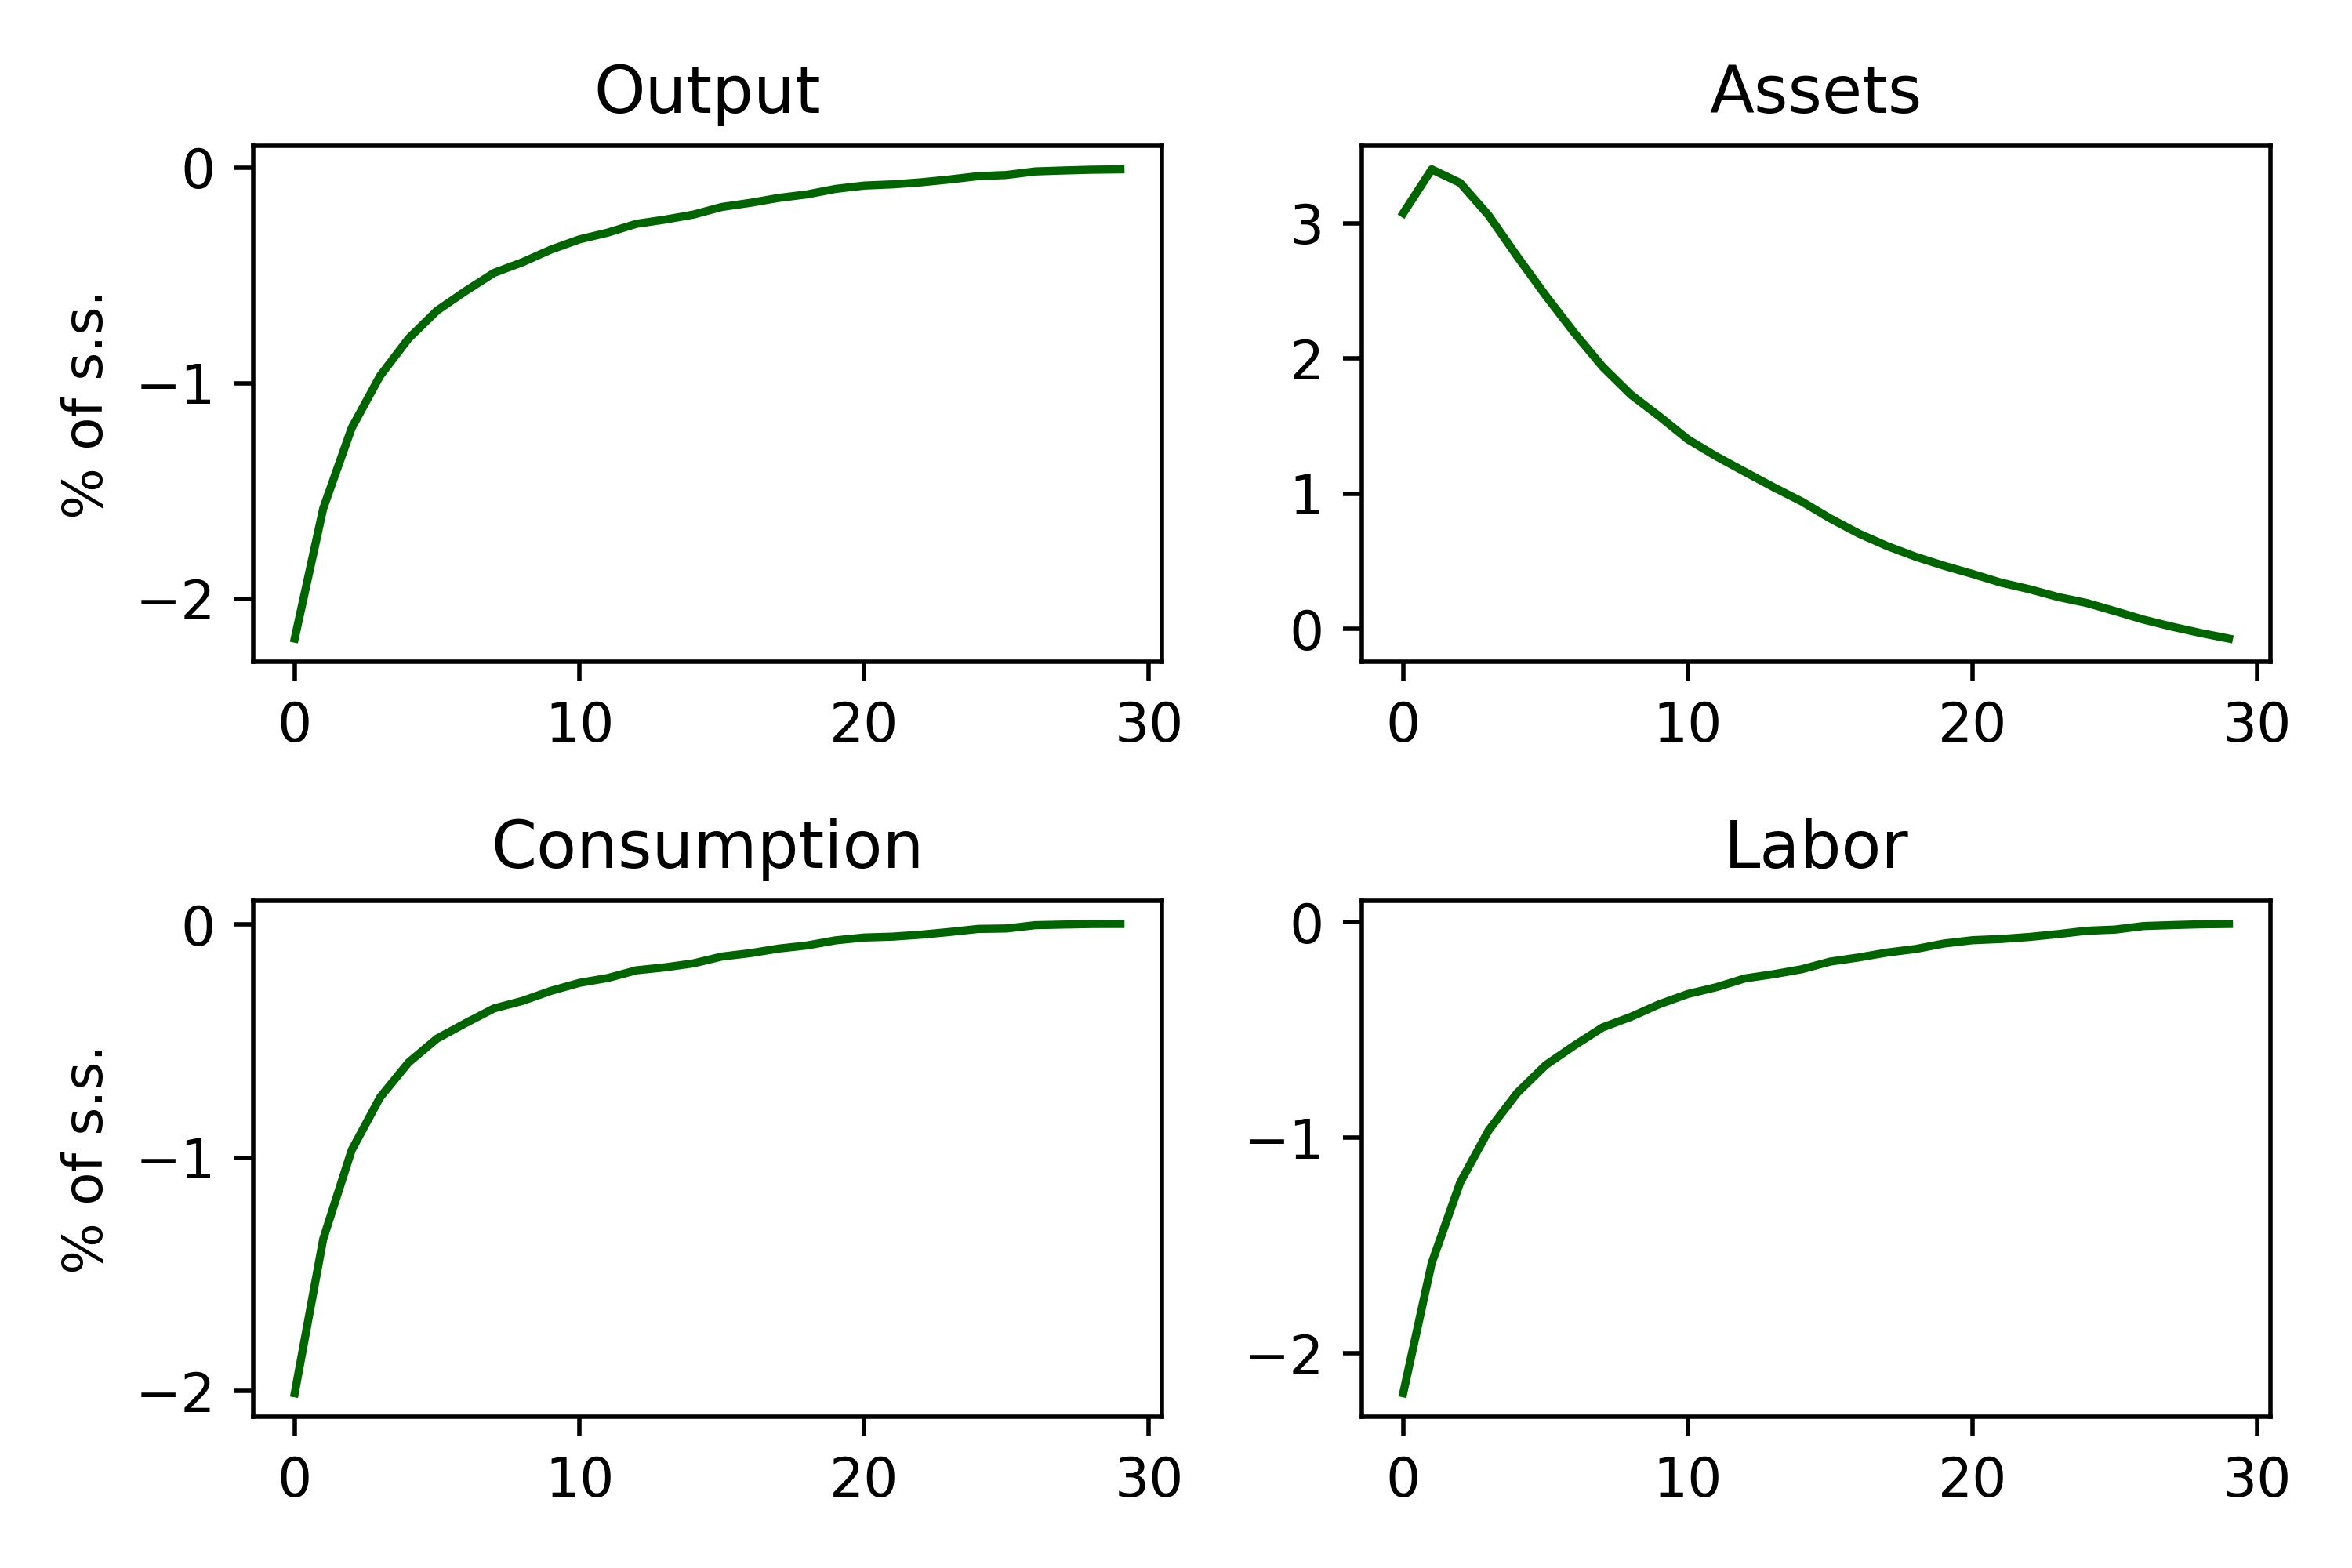
\includegraphics[scale=.35]{\FigDir/GIPRM2}
  \end{subfigure}
  \begin{subfigure}{}
    \centering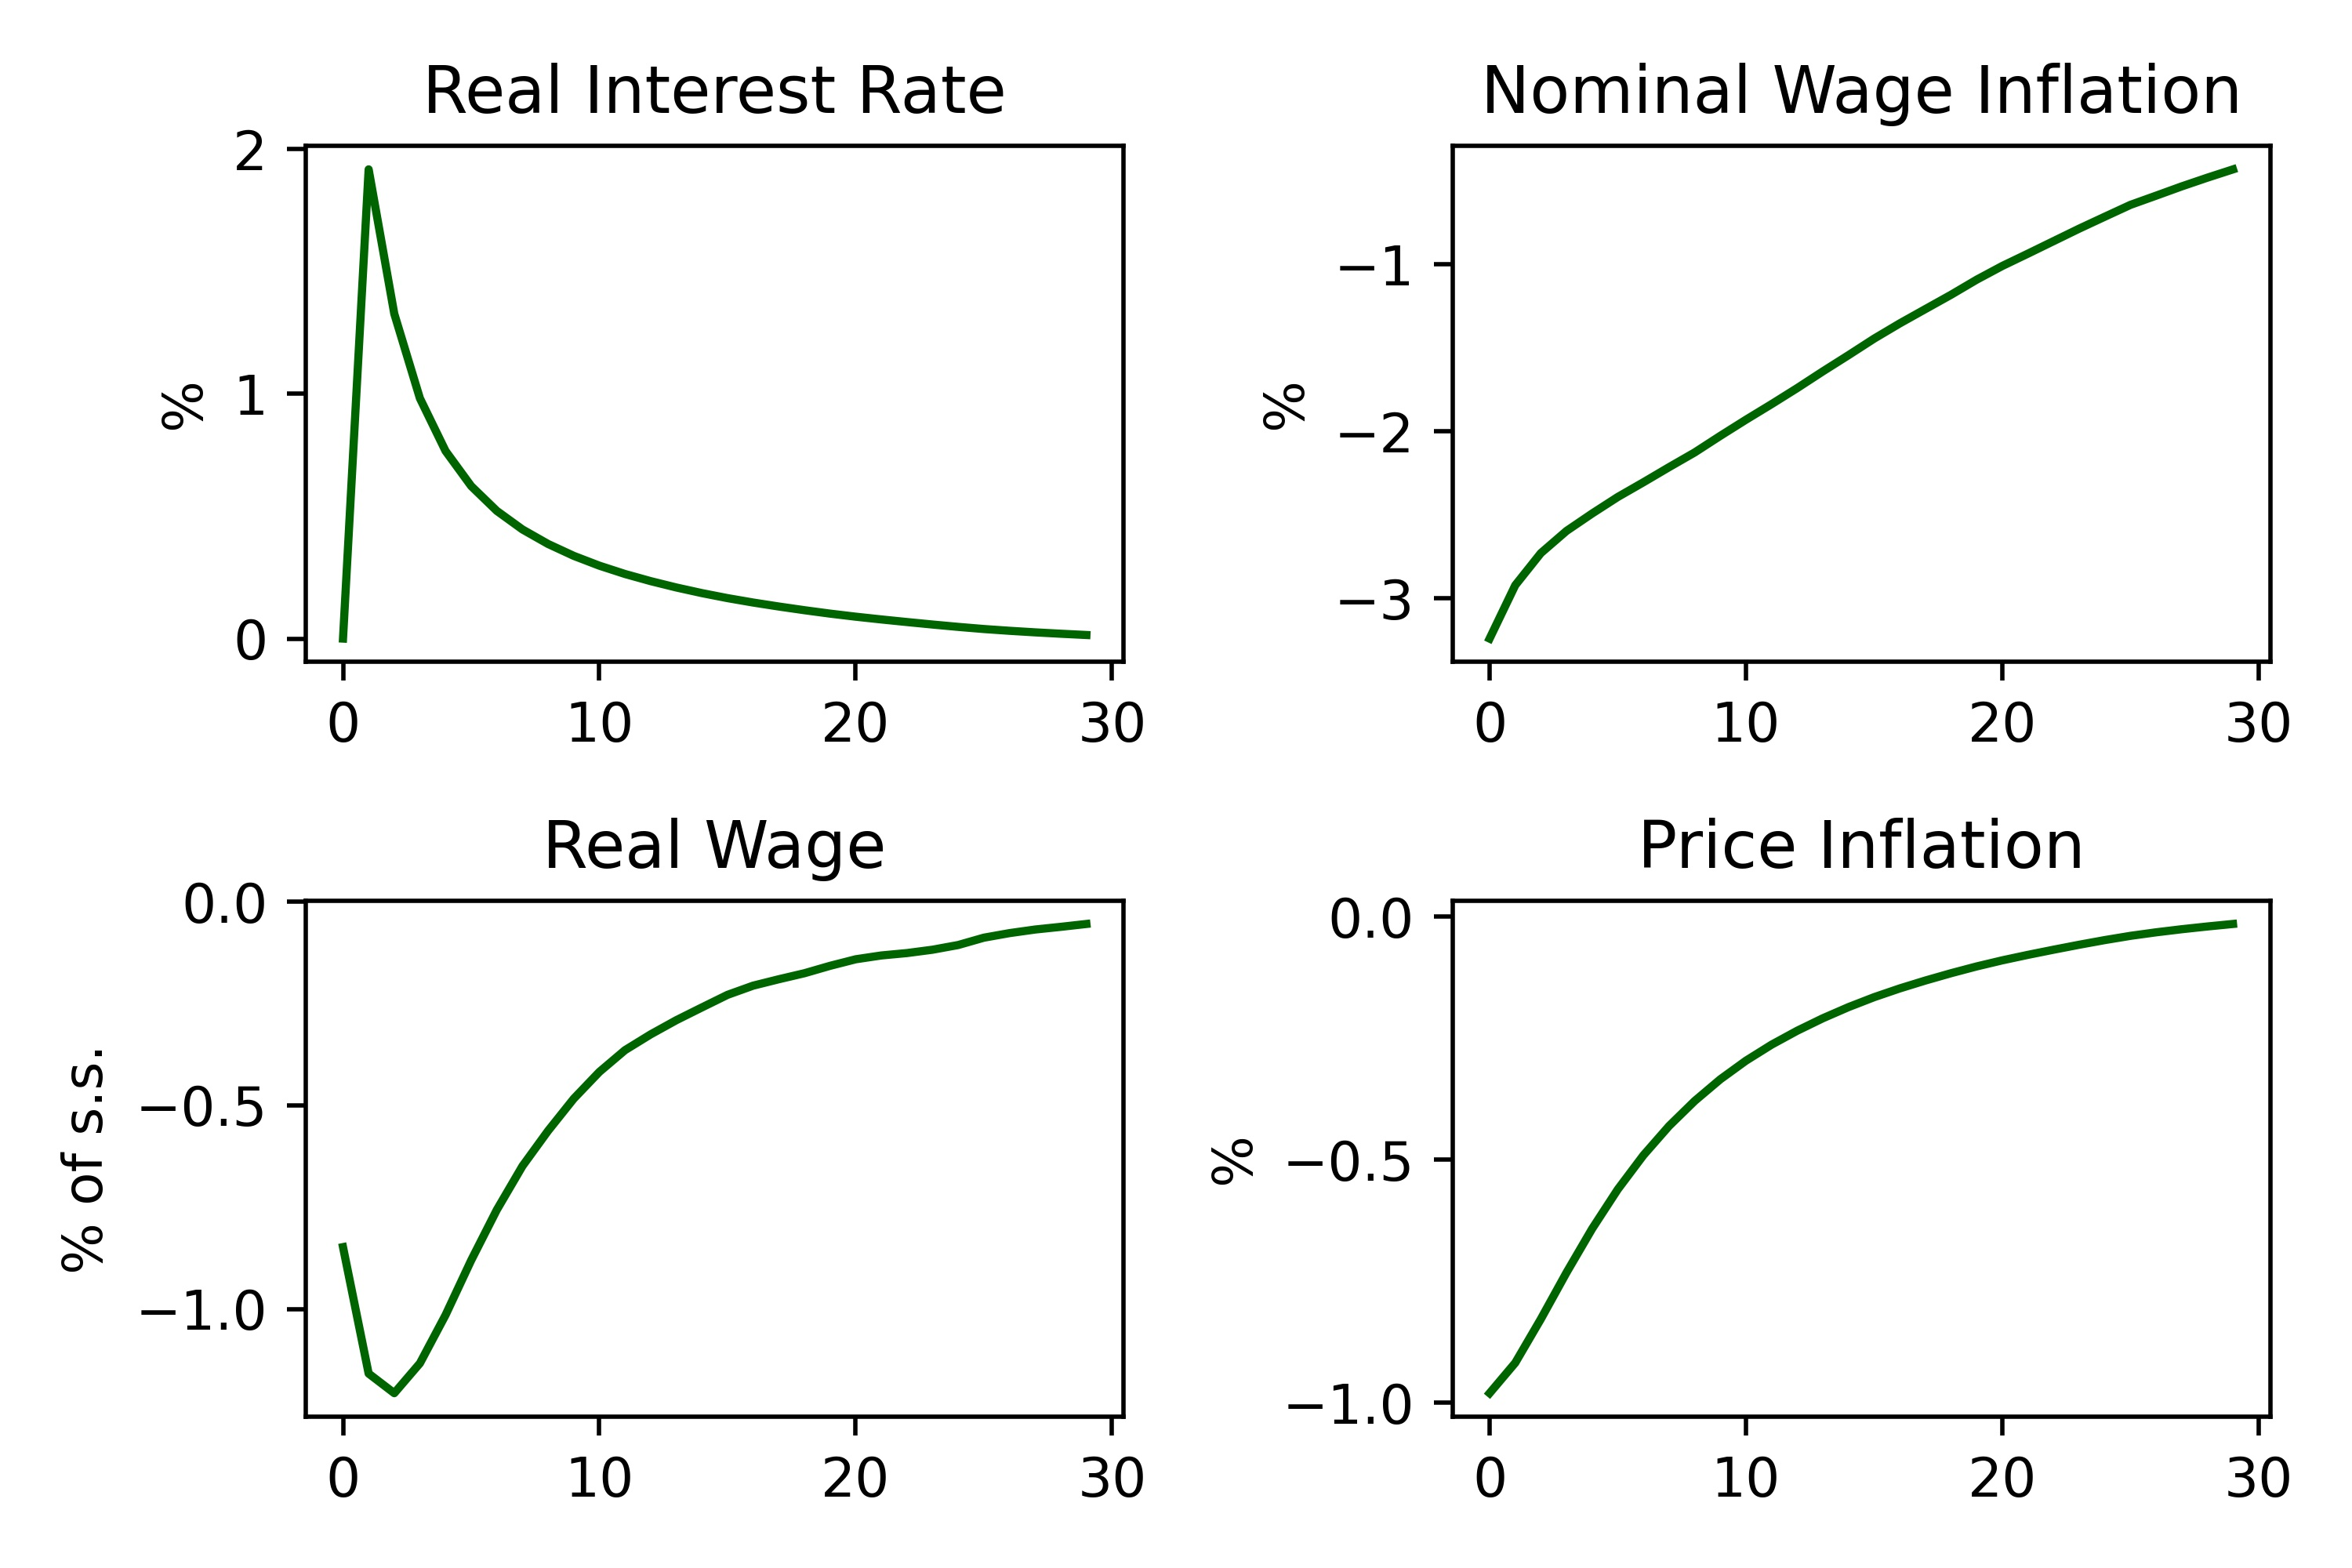
\includegraphics[scale=.35]{\FigDir/GIPRM1}
    \caption{ Impulse Response to One Percent Increase in Nominal Rate}
  \end{subfigure}
\end{figure}


\hypertarget{Productivity Shock}{}
\subsection{Productivity Shock}


The impulse responses to the productivity shock can be found in figure 2. The productivity shock is a 1 percent increase in $Z_{t}$ following an AR(1) with a coefficient of .9. The rise in productivity raises both output and firm markups, inducing downward pressure on prices which inturn induces downward pressure on nominal wages. However, given the goods market must clear, consumption must rise causing upward pressure on the nominal wage since the economy marginal rate of substitution is a function of the average marginal utility of consumption. The net effect will see nominal wages rise leading to upward pressure on prices. The net effect of all these different pressures will see the real wage rise and therefore amplify the consumption response signficantly due to the large aggregate MPC in the model. In addition, to the fixed nominal interest rate, inflation will see the real interest rate fall further amplifying consumption. This amplification of consumption will lead to rises in output and labor due to upward pressure on labor demand.

\begin{figure}{Impulse Responses to a Productivity Shock}
  \begin{subfigure}{}
    \centering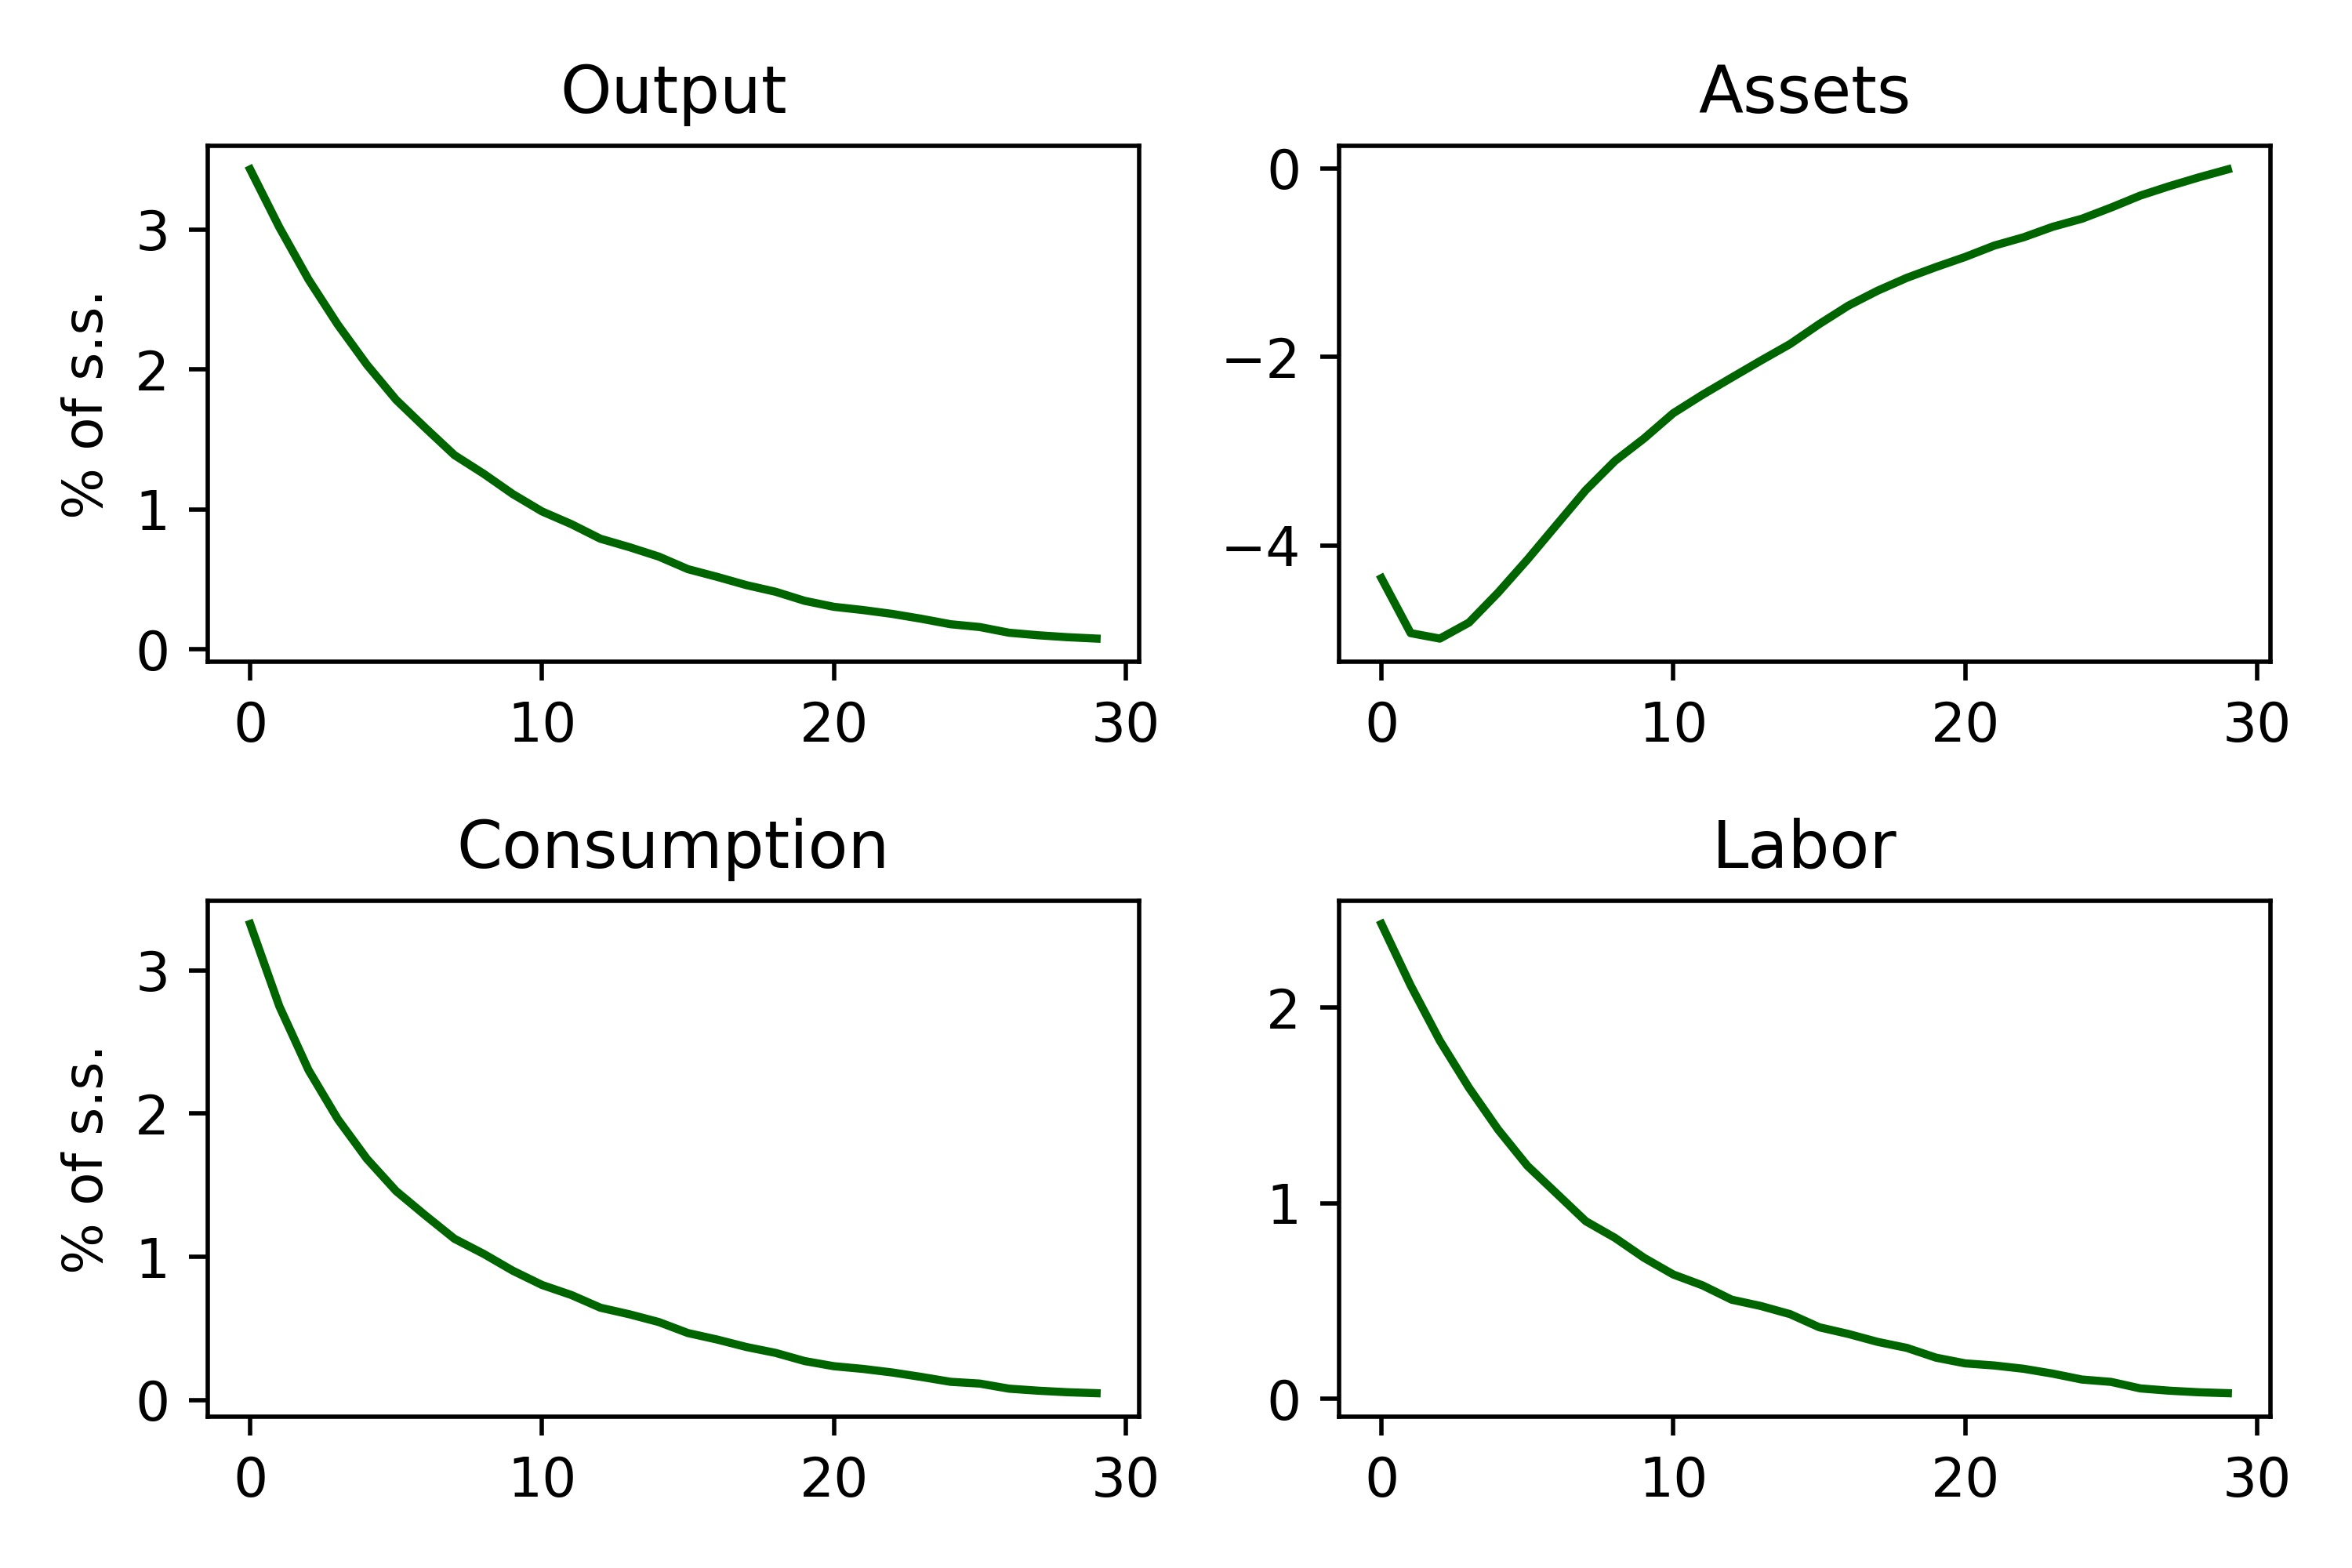
\includegraphics[scale=.35]{\FigDir/GIPRZ2}
  \end{subfigure}
  \begin{subfigure}{}
    \centering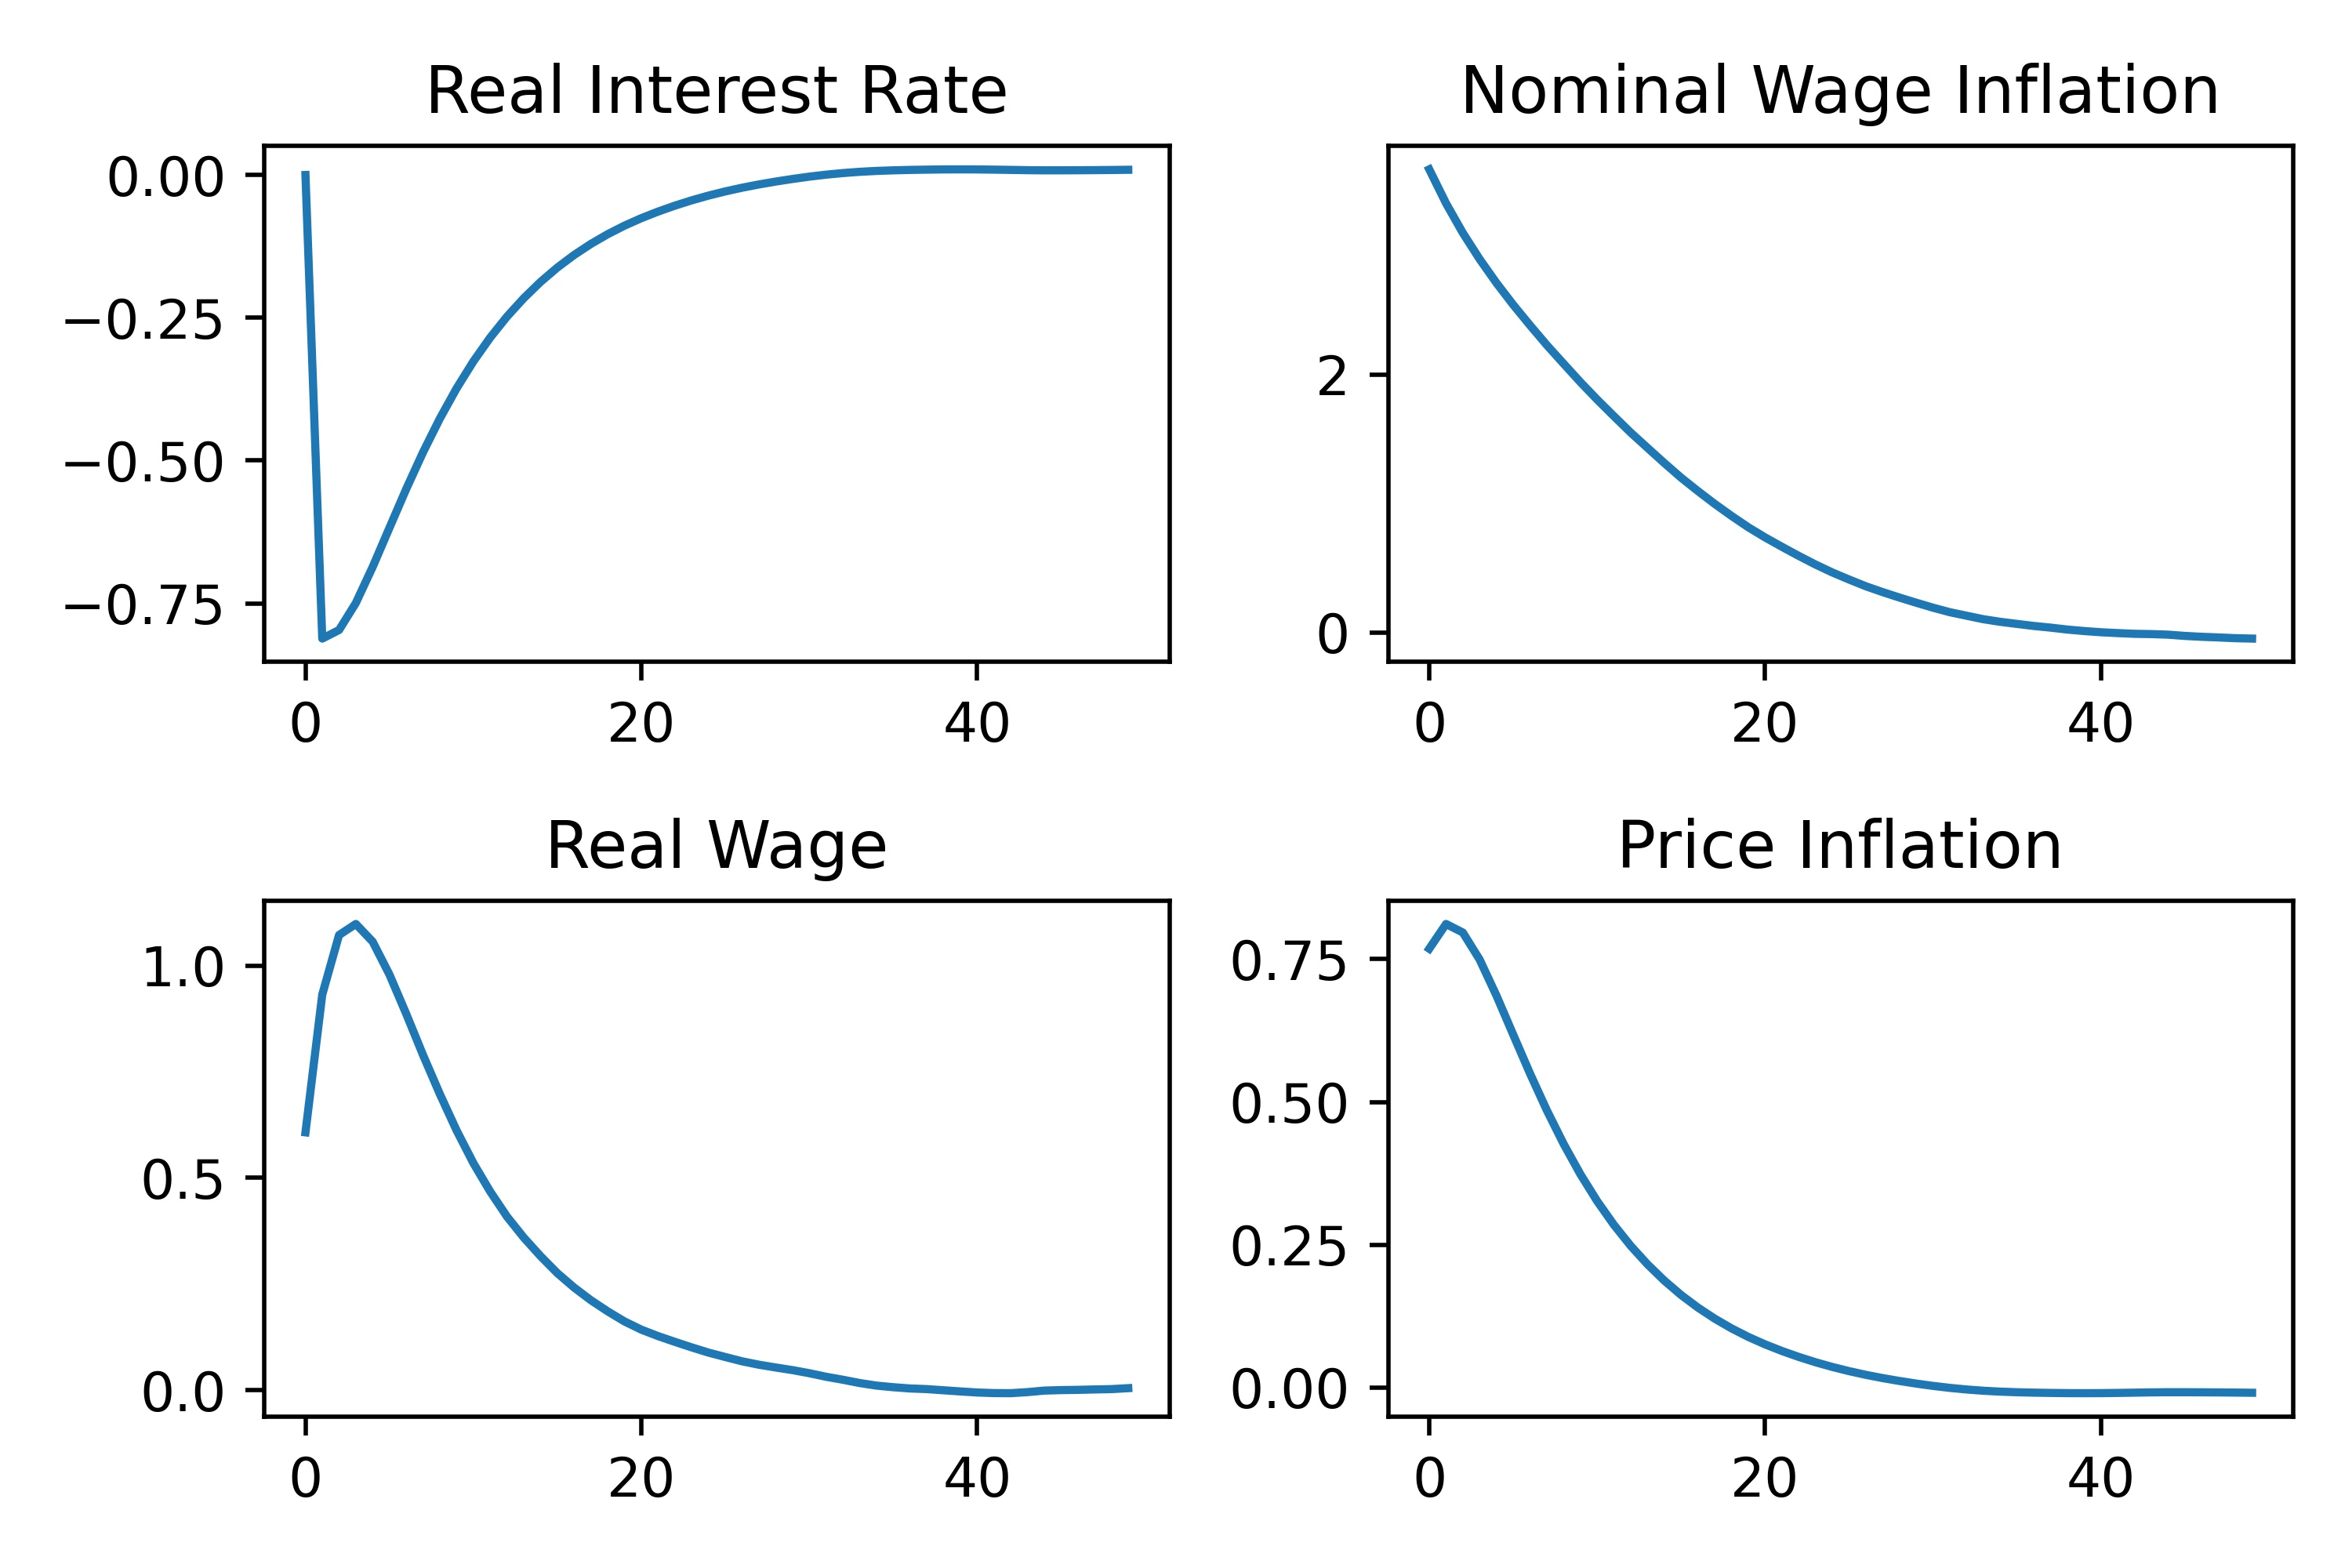
\includegraphics[scale=.35]{\FigDir/GIPRZ1}
    \caption{ Impulse Response to One Percent Increase in $Z_{t}$}
  \end{subfigure}
\end{figure}



\hypertarget{Issues and Extensions}{}
\section{Issues and Extensions}

The most prominent issue I have encountered thus far is determining whether the impulse responses are accurate in regards to the specification of the model. Producing the impulses responses is an exercise in linear algebra and the computation of jacobians. Because the jacobians were constructed without automatic differentiation, the accuracy of the impulse responses produced is uncertain as the smallest algebraic mistake may render them incorrect. Despite this uncertainty, the impulse responses of the model do mirror the responses produced from dynare under certain calibrations.  In particular, as long as prices are calibrated to be slightly stickier than wages, the impulse responses from a monetary policy shock behave in exactly the same manner as those produced from dynare. In addition, the impulse responses from a productivity shock seem essentially no different to those produced from dynare. The only issue is whenever wages are calibrated to be stickier than prices. When wages are stickier than prices,  to be specific, if the parameter for wage stickiness is set to .85 and the that of price stickiness to .8, the impulse responses to a monetary contraction are quantitatively the same as those seen in section 5 except they all invert across the x axis. That is, with the rise in the nominal rate, the results see a rise in consumption, output, labor, inflation and the real wage. This is much cause for concern regarding the accuracy of the code that produces the impulse responses as they do not survive under calibrations where wages are stickier than prices. It is possible, however, that these inverted responses may be accurate to the model due to the strong responsiveness of consumption present in the model. For instance, when the inverse frish elasticity is set to a large value (from v =2 to v=7) rendering labor to be significantly less sensitive to changes in wages, the impulse responses do not invert anymore ( consumption, output, labor, real wages all fall after a rise in the nominal rate). This is evidence that perhaps the consumption response is so strong that the slightest change in calibration could lead to large amplification effects that can invert the impulse response. My current hypothesis is that when prices are slightly more flexible than wages, the real wage may perhaps rise as since an increase in the nominal rate induces downward pressure on both prices and wages and if the fall in prices is larger than the fall in wages, the real wage may rise inducing a strong consumption response which amplifies and lead aggregate variables such as labor supply, and output to rise when the real rate rises. 
























%\providecommand{\figName}{GIPRM1}
%\providecommand{\figFile}{GIPRM1}
%\hypertarget{\figFile}{}
%\hypertarget{\figName}{}
%\begin{figure}[tbp]
%\centerline{\includegraphics[scale=.35]{\FigDir/\figFile}}
%\caption{Monetary Policy Shock}
%\label{fig:\figFile}
%\end{figure}


%%
%\renewcommand{\figFile}{GIPRM2}
%\hypertarget{\figFile}{}  
%\begin{figure}[tbp]
%\centerline{\includegraphics[scale=.35]{\FigDir/\figFile}}
%\caption{Monetary Policy Shock}
%\label{fig:\figFile}
%\end{figure}
%%


\clearpage\vfill\eject

\appendix

\centerline{\LARGE Appendices}\vspace{0.2in}




\hypertarget{Computational Details}{}
\section{Computational Details}

\hypertarget{Household Bellman Equation }{}
\subsection{Household Bellman Equation}

Household i's dynamic program is

$$ V(\pmb{\mathrm{m}}_{it},\pmb{\mathrm{p}}_{it})=\max_{ \{ \pmb{\mathrm{c}}_{it}\}} { \frac{\cLevBF_{i t}^{1-\rho}}{1 -\rho} - \varphi \pLevBF_{it} \frac{n_{it}^{1+v}}{1+v} + \beta_{i} \not D \mathrm{E}_{t}[V( \pmb{\mathrm{m}}_{it+1} , \pmb{\mathrm{p}}_{it+1})]}$$

subject to 

\begin{align*}
 \pmb{\mathrm{m}}_{i t} & = \pmb{\mathrm{z}}_{i t}  + (1+\mathit{r}^{a}_{t})\pmb{\mathrm{a}}_{i t-1} \\
 \pmb{\mathrm{c}}_{i t}  + \pmb{\mathrm{a}}_{i t} &= \pmb{\mathrm{z}}_{i t}  + (1+\mathit{r}^{a}_{t}) \pmb{\mathrm{a}}_{i t-1}   \\
\pmb{\mathrm{a}}_{it} &\geq 0 
\end{align*} \\ \\

This can be normalized to \\


$$ V(m_{it}) = \max_{\{c_{it}\}} {  \frac{c_{i t}^{1-\rho}}{1 -\rho} - \varphi \frac{n_{it}^{1+v}}{1+v} + \beta_{i}\not D \mathrm{E}_{t}[\psi_{it+1}^{1-\rho} V(m_{it+1})]}$$

 subject to 
 
 \begin{align*}
m_{i t} &=  \xi_{it}  + (1+r^{a}_{t}) \frac{a_{i t-1}}{\psi_{it}} \\
 c_{i t}  + a_{i t} &= \xi_{it}  + (1+r^{a}_{t}) \frac{a_{i t-1}}{\psi_{it}} \\
 a_{it} &\geq 0 
 \end{align*}
 
 Here non boldface variables are normalized by permanent income $\mathit{p_{it}}$. 

e.g. $x_{it} = \frac{\mathbf{x_{it}}}{\pmb{\mathrm{p}}_{it}}$ \\

First order condition for consumption:

$$c_{it}^{-\rho} -  \beta_{i} \not D \mathrm{E}_{t}\left[ (1+r^{a}_{t+1})  \psi_{it+1}^{-\rho} V'(m_{it+1})\right] = 0$$ \\ 



%%Now let $v(m_{it}, c_{it}) = \frac{c_{i t}^{1-\rho}}{1 -\rho} - \varphi \frac{n_{it}^{1+v}}{1+v} + \beta_{i}\not D \mathrm{E}_{t}[\psi_{it+1}^{1-\rho} V(m_{it+1})] $ and let $c_{it}(m_{it})$ denote the solution to the original dynamic problem.  \\ 

%%Note $ \frac{ \partial v(m_{it},c_{it}(m_{it}))}{\partial m} =  \beta_{i}\not D \mathrm{E}_{t}[\psi_{it+1}^{1-\rho} V'(m_{it+1})] $ \\

%%Then $$ V(m_{it}) = v(m_{it}, c_{it}(m_{it})$$ 

%%$$ V'(m_{it}) = \frac{ \partial v(m_{it},c_{it}(m_{it}))}{\partial m}$$ 

%%Which leads to the envelope condition \\

%%$$V'(m_{it}) =  \beta_{i}\not D \mathrm{E}_{t}[\psi_{it+1}^{1-\rho} V'(m_{it+1})] $$




\hypertarget{Model as System}{}
\subsection{Model as System}

The model can be defined by the system of equations below. The solution of the model must see this system be equal to a vector of zeros for periods $t =0, 1, 2, 3, ...$. The system is defined over the sequence space of all endogenous variables $\mathbf{U}$  and exogenous variables $\mathbf{Z}$ of the model.

$$
H_{t}(\mathbf{U},\mathbf{Z})= \begin{pmatrix} 
 Y_{t} - Z_{t}N_{t} \\ \\ 
B_{t-1} - q^{b}_{t}B_{t} + u\mho + G - \tau w_{t} N_{t} \\ \\  
i_{t} - r^{*} - \phi \pi^{p}_{t} -\phi_{y}(Y_{t}-Y_{ss}) - v_{t} \\ \\
\pi_{t}^{p} -\frac{\pi^{p}_{t+1}}{1+r^{*}} + \lambda(\mu_{t}^{p} -\mu_{p})  \\ \\
 \pi_{t}^{w} -\not D \pi_{t+1}^{w} -(\frac{1-\lambda_{w}}{\lambda_{w}}) (1- \not D \lambda_{w}) (\mu^{w} -\mu_{t}^{w}) \\ \\
    1+r_{t} - \frac{1 + i_{t}}{1+ \pi^{p}_{t+1}}\\ \\
 1+r_{t+1}^{a} - \frac{q_{t+1}^{s} +D_{t+1}}{q_{t}^{s}} \\ \\
 r_{t} - r_{t+1}^{a} \\ \\
 \frac{w_{t}}{w_{t-1}} - \frac{\Pi_{t}^{w}}{\Pi_{t}^{p}} \\ \\
 \mathcal{C}_{t}(\{r_{s}^{a} ,w_{s}, N_{s}\}_{s=0}^{s=T}) - Y_{t} + G \\ \\
 \end{pmatrix} = \begin{pmatrix} 0 \\ 0 \\. \\. \\. \\ 0\\ \end{pmatrix} , \quad t=0,1 ,2,3,....
$$ \\ \\
 

 
 where \\
 
$\mathcal{C}_{t}(\{r_{s}^{a} ,w_{s}, N_{s}\}_{s=0}^{s=T}) = \int_{0}^{1} \pLevBF_{it} c_{it}(m_{it})\, di $ \\
 
$c_{it}(m_{it})$ is the steady state normalized consumption policy for household $i$ in period t. \\ \\
 

 
 
 $\mathbf{U} = \left(Y_{t} , N_{t} ,  D_{t
 }, B_{t}, w_{t} , \pi_{t}^{p} ,\pi_{t}^{w}, r_{t} , r_{t+1}^{a}, i_{t} , q_{t}^{s},  q_{t}^{s} \right)_{t=0}^{t=T}$ \\ 

 
 $\mathbf{Z} = \left(Z_{t} ,v_{t}\right)_{t=0}^{t=T}$ \\
 
 \textbf{Note} the asset market clearing condition is not included in the system as the goods market clearing condition holds if and only if the asset market clearing condition holds. On the same note, the government budget constraint nor the equation for the stock price is included in the reduced system as they both bonds and its stock price appears in the asset clearing equation.  \\ \\
 
 
 
\hypertarget{Reduced System}{}
\subsubsection{Reduced System}
 
The previous system of a little more than a dozen endogenous variables can be reduced to a system of three endogenous variables. \\ 
 
Endogenous Variables are $ r_{t} , w_{t} ,N_{t}$ \\ 
 
Exogenous Variables are $ Z_{t}, v_{t}$ \\ 

The reduced system: \\ \\

\begin{eqnarray} 
H_{t}(\mathbf{U},\mathbf{Z})= \begin{pmatrix} 
\mathcal{H}_{t,1} \\ \\ 
\mathcal{H}_{t,2} \\ \\
\mathcal{H}_{t,3} \\ \\
 \end{pmatrix} = \begin{pmatrix} 0 \\ 0 \\ 0 \\ \end{pmatrix} , \quad  t = 0, 1, 2, ..., T 
 \end{eqnarray}
 
 where \\ 
 
 
 $\mathcal{H}_{t,1}  =\mathcal{C}_{t}\left( \left \{r^{a}_{s} , w_{s} , N_{s}  \right \}_{s=0}^{s=T} \right) - Z_{t} N_{t} + G\\ \\ $

$ \mathcal{H}_{t,2}  =log(w_{t}) - log(w_{t-1}) + \left( \frac{1 - \lambda_{w}}{\lambda_{w}}(1 - \not D \lambda_{w}) \sum_{k=0}^{\infty} \not D^{k} ( \mu_{t+k}^{w} - \mu^{w}) \right) - \left(  \lambda \sum_{k=0}^{\infty} \frac{1}{(1+r^{*})^{k}} ( \mu_{t+k}^{p} - \mu^{p})\right)\\ \\ $

$ \mathcal{H}_{t,3}  =  (1+r_{t}) \left(1+ -\lambda \sum_{k=1}^{\infty} \frac{1}{(1+r^{*})^{k}} ( \mu_{t+k}^{p} - \mu^{p}) \right) \\ \\
 - \left(1+r^{*}+ \phi \left(- \lambda \sum_{k=0}^{\infty} \frac{1}{(1+r^{*})^{k}} ( \mu_{t+k}^{p} - \mu^{p}) \right) +\phi_{y} \left(Z_{t} N_{t} - Y_{ss} \right) + v_{t}\right) \\ \\ $
 
$ \mu_{t}^{p} = log(\frac{1}{w_{t}}) + log(Z_{t})$ \\ 

$\mu_{t}^{w} = log(w_{t}) + log(1 - \tau_{t}) - mrs_{t} \\  $

$mrs_{t} = log \left(- \frac{\int_{0}^{1}   U_{n} \left(\cLevBF_{i t}, n_{i t} \right) \ d i  }{\int_{0}^{1} \pLevBF_{it} \theta_{it} U_{c} \left(\cLevBF_{i t}, n_{i t} \right) \  di } \right) = log \left(\frac{\int_{0}^{1} \varphi \pLevBF_{it} n_{it}^{v} \ d i  }{\int_{0}^{1} \pLevBF_{it}  \theta_{it} \cLevBF_{it}^{-\rho} \  di } \right) = log \left(\frac{\int_{0}^{1} \varphi \pLevBF_{it} \left(\frac{N_{t}}{1 - \mho} \right)^{v} \, d i  }{\int_{0}^{1} \pLevBF_{it}  \theta_{it} \cLevBF_{it}^{-\rho} \  di } \right)$ \\ 

$ = log \left( \varphi \left(\frac{N_{t}}{1 - \mho}\right) ^{v}\right) + log \left(\int_{0}^{1} \pLevBF_{it}  \,  di  \right) - log \left(\int_{0}^{1} \pLevBF_{it}  \theta_{it} \cLevBF_{it}^{-\rho} \  di  \right) $ \\ \\
 
 and the arguments of the function $H_{t}$ are \\
 
$\mathbf{U} = (r_{0} , r_{1} , ...r_{T}, w_{0}, w_{1}, ..., w_{T}, N_{0}, N_{1},...,N_{T})$ \\ 

$ \mathbf{Z} = ( Z_{0}, Z_{1},... Z_{T}, v_{0},...,v_{T}) \\ \\ $ 




\hypertarget{Jacobian of System}{}
\subsection{Jacobian of System} 

\hypertarget{Implicit Function Theorem}{}
\subsubsection{Implicit Function Theorem} 

By applying the implicit function theorem to the reduced system, we can obtain the endogenous responses of the real interest rate, wage, and labor supply given some exogenous shock \\

$$d\mathbf{U} =  -{\mathbf{H}_{\mathbf{U}}}^{-1} \mathbf{H}_{\mathbf{Z}} d \mathbf{Z}$$ \\ 

where $d\mathbf{U}$ are the endogenous responses of the real interest rate, the real wage, and labor supply to an exogenous shock $d \mathbf{Z}$.

Specifically, notation is defined below\\


$$d\mathbf{U} =(dr_{0} , dr_{1} , ...dr_{T}, dw_{0}, dw_{1}, ..., dw_{T}, dN_{0}, dN_{1},...,dN_{T})$$

$$d \mathbf{Z} = ( dZ_{0}, dZ_{1},... dZ_{T}, dv_{0},...dv_{T}) $$ \\





 $$  \mathbf{H}_{\mathbf{U}}= \begin{pmatrix} 
H_{\mathbf{U}, 1} \\ \\ 
H_{\mathbf{U}, 2}  \\ \\
H_{\mathbf{U}, 3} \\ \\
 \end{pmatrix} \quad \quad \mathbf{H}_{\mathbf{Z}}= \begin{pmatrix} 
H_{\mathbf{Z}, 1} \\ \\ 
H_{\mathbf{Z}, 2}  \\ \\
H_{\mathbf{Z}, 3} \\ \\
 \end{pmatrix}$$ \\ \\
 
 
 $$ H_{\mathbf{U}, i}= \begin{pmatrix} 
\frac{ \partial \mathcal{H}_{0,i}}{\partial r_{0}}  & ... & \frac{ \partial \mathcal{H}_{0,i}}{\partial r_{T}} & \frac{ \partial \mathcal{H}_{0,i}}{\partial w_{0}} & ... & \frac{ \partial \mathcal{H}_{0,i}}{\partial w_{T}} & \frac{ \partial \mathcal{H}_{0,i}}{\partial N_{0}} & ... &\frac{ \partial \mathcal{H}_{0,i}}{\partial N_{T}} \\ \\ 
\frac{ \partial \mathcal{H}_{1,i}}{\partial r_{0}}  & ... & \frac{ \partial \mathcal{H}_{1,i}}{\partial r_{T}} & \frac{ \partial \mathcal{H}_{1,i}}{\partial w_{0}} & ... & \frac{ \partial \mathcal{H}_{1,i}}{\partial w_{T}} & \frac{ \partial \mathcal{H}_{1,i}}{\partial N_{0}} & ... &\frac{ \partial \mathcal{H}_{1,i}}{\partial N_{T}}  \\ \\
.   \\ \\ \\ 
. \\ \\ \\
. \\ \\ \\
\frac{ \partial \mathcal{H}_{T,i}}{\partial r_{0}}  & ... & \frac{ \partial \mathcal{H}_{T,i}}{\partial r_{T}} & \frac{ \partial \mathcal{H}_{T,i}}{\partial w_{0}} & ... & \frac{ \partial \mathcal{H}_{T,i}}{\partial w_{T}} & \frac{ \partial \mathcal{H}_{T,i}}{\partial N_{0}} & ... &\frac{ \partial \mathcal{H}_{T,i}}{\partial N_{T}} \\ \\
 \end{pmatrix} $$ \\
 
  $$ H_{\mathbf{Z}, t}= \begin{pmatrix} 
\frac{ \partial \mathcal{H}_{0,i}}{\partial Z_{0}}  & ... & \frac{ \partial \mathcal{H}_{0,i}}{\partial Z_{T}} & \frac{ \partial \mathcal{H}_{0,i}}{\partial v_{0}} & ... & \frac{ \partial \mathcal{H}_{0,i}}{\partial v_{T}} \\ \\ 
\frac{ \partial \mathcal{H}_{1,i}}{\partial Z_{0}}  & ... & \frac{ \partial \mathcal{H}_{1,i}}{\partial Z_{T}} & \frac{ \partial \mathcal{H}_{1,i}}{\partial v_{0}} & ... & \frac{ \partial \mathcal{H}_{1,i}}{\partial v_{T}} \\ \\
. \\ \\ \\ 
. \\ \\ \\
. \\ \\ \\
\frac{ \partial \mathcal{H}_{T,i}}{\partial Z_{0}}  & ... & \frac{ \partial \mathcal{H}_{T,i}}{\partial Z_{T}} & \frac{ \partial \mathcal{H}_{T,i}}{\partial v_{0}} & ... & \frac{ \partial \mathcal{H}_{T,i}}{\partial v_{T}}  \\ \\
 \end{pmatrix} $$ \\ \\
 
 
\textbf{ Or equivalently}

 $$  \mathbf{H}_{\mathbf{U}}= \begin{pmatrix} 
H_{\mathbf{U}, 0} \\ \\ 
H_{\mathbf{U}, 1}  \\ \\
. \\ \\
. \\ \\
. \\ \\ 
H_{\mathbf{U}, T} \\ \\
 \end{pmatrix} \quad \quad \mathbf{H}_{\mathbf{Z}}= \begin{pmatrix} 
H_{\mathbf{Z}, 0} \\ \\ 
H_{\mathbf{Z}, 1}  \\ \\
. \\ \\
. \\ \\
. \\ \\ 
H_{\mathbf{Z}, T} \\ \\
 \end{pmatrix}$$ \\ \\
 
 
 
$$ H_{\mathbf{U}, t}= \begin{pmatrix} 
\frac{ \partial \mathcal{H}_{t,1}}{\partial r_{0}}  & ... & \frac{ \partial \mathcal{H}_{t,1}}{\partial r_{T}} & \frac{ \partial \mathcal{H}_{t,1}}{\partial w_{0}} & ... & \frac{ \partial \mathcal{H}_{t,1}}{\partial w_{T}} & \frac{ \partial \mathcal{H}_{t,1}}{\partial N_{0}} & ... &\frac{ \partial \mathcal{H}_{t,1}}{\partial N_{T}} \\ \\ 
\frac{ \partial \mathcal{H}_{t,2}}{\partial r_{0}}  & ... & \frac{ \partial \mathcal{H}_{t,2}}{\partial r_{T}} & \frac{ \partial \mathcal{H}_{t,2}}{\partial w_{0}} & ... & \frac{ \partial \mathcal{H}_{t,2}}{\partial w_{T}} & \frac{ \partial \mathcal{H}_{t,2}}{\partial N_{0}} & ... &\frac{ \partial \mathcal{H}_{t,2}}{\partial N_{T}}  \\ \\
\frac{ \partial \mathcal{H}_{t,3}}{\partial r_{0}}  & ... & \frac{ \partial \mathcal{H}_{t,3}}{\partial r_{T}} & \frac{ \partial \mathcal{H}_{t,3}}{\partial w_{0}} & ... & \frac{ \partial \mathcal{H}_{t,3}}{\partial w_{T}} & \frac{ \partial \mathcal{H}_{t,3}}{\partial N_{0}} & ... &\frac{ \partial \mathcal{H}_{t,3}}{\partial N_{T}} \\ \\
 \end{pmatrix} $$ \\
 
  $$ H_{\mathbf{Z}, t}= \begin{pmatrix} 
\frac{ \partial \mathcal{H}_{t,1}}{\partial Z_{0}}  & ... & \frac{ \partial \mathcal{H}_{t,1}}{\partial Z_{T}} & \frac{ \partial \mathcal{H}_{t,1}}{\partial v_{0}} & ... & \frac{ \partial \mathcal{H}_{t,1}}{\partial v_{T}} \\ \\ 
\frac{ \partial \mathcal{H}_{t,2}}{\partial Z_{0}}  & ... & \frac{ \partial \mathcal{H}_{t,2}}{\partial Z_{T}} & \frac{ \partial \mathcal{H}_{t,2}}{\partial v_{0}} & ... & \frac{ \partial \mathcal{H}_{t,2}}{\partial v_{T}} \\ \\
\frac{ \partial \mathcal{H}_{t,3}}{\partial Z_{0}}  & ... & \frac{ \partial \mathcal{H}_{t,3}}{\partial Z_{T}} & \frac{ \partial \mathcal{H}_{t,3}}{\partial v_{0}} & ... & \frac{ \partial \mathcal{H}_{t,3}}{\partial v_{T}}  \\ \\
 \end{pmatrix} $$ \\ \\
 
 
 
 
\hypertarget{Obtaining All Other Responses}{}
\subsubsection{Obtaining All Other Responses} 

To obtain all other responses given the endogenous response $\mathbf{dU}$, we compute the jacobians of the endogenous variable with respect to the relevant endogenous variables that have already been solved for.  For example, to compute the response of consumption to some exogenous shock $d\mathbf{Z}$, we sum  the jacobians of consumption with respect to the real interest rate, the wage and labor supply 

$$ d\mathbf{C} = \mathcal{J}^{\mathcal{C} , r} d\mathbf{r} +\mathcal{J}^{\mathcal{C} , w} d\mathbf{w} +\mathcal{J}^{\mathcal{C} , N} d\mathbf{N} $$\\
 
 where $\mathcal{J}^{\mathcal{C} , w} $ is the jacobian of aggregate consumption  $\mathcal{C}_{t}(\{r_{s}^{a} ,w_{s}, N_{s}\}_{s=0}^{s=T}) $  with respect to the wage. \\
 
 To be clear , 
 
$$d\mathbf{w} =  ( dw_{1}, dw_{2}, . . . , dw_{T})' $$
 
 
 
 $$\mathcal{J}^{\mathcal{C} , w} =   \begin{pmatrix} 
\frac{ \partial \mathcal{C}_{0}(\{r_{s}^{a} ,w_{s}, N_{s}\}_{s=0}^{s=T})}{\partial w_{0}}  & \frac{ \partial \mathcal{C}_{0}(\{r_{s}^{a} ,w_{s}, N_{s}\}_{s=0}^{s=T})}{\partial w_{1}}&    ... & \frac{ \partial \mathcal{C}_{0}(\{r_{s}^{a} ,w_{s}, N_{s}\}_{s=0}^{s=T})}{\partial w_{T}} \\ \\ 
\frac{ \partial \mathcal{C}_{1}(\{r_{s}^{a} ,w_{s}, N_{s}\}_{s=0}^{s=T})}{\partial w_{0}}  &\frac{ \partial \mathcal{C}_{1}(\{r_{s}^{a} ,w_{s}, N_{s}\}_{s=0}^{s=T})}{\partial w_{1}}& ... & \frac{ \partial \mathcal{C}_{1}(\{r_{s}^{a} ,w_{s}, N_{s}\}_{s=0}^{s=T})}{\partial w_{T}} \\ \\
.  \\ \\
.  \\ \\
. \\ \\
\frac{ \partial \mathcal{C}_{T}(\{r_{s}^{a} ,w_{s}, N_{s}\}_{s=0}^{s=T})}{\partial w_{0}}  &\frac{ \partial \mathcal{C}_{T}(\{r_{s}^{a} ,w_{s}, N_{s}\}_{s=0}^{s=T})}{\partial w_{1}}& ... & \frac{ \partial \mathcal{C}_{T}(\{r_{s}^{a} ,w_{s}, N_{s}\}_{s=0}^{s=T})}{\partial w_{T}}  \\ \\
 \end{pmatrix} $$ \\
 
  
\hypertarget{Additional Derivations}{}
\section{Additional Derivations} 

An employed household's transitory income is \\

$$ \theta_{it}(1-\tau) \int_{0}^{1} \frac{W_{gt}}{P_{t}}n_{igt}\,dg$$

where $W_{gt}$ denotes the nominal wage for labor type $g$ and $P_{t}$ the price of the final good. \\ \\

Now noitce

$$ \theta_{it}(1-\tau) \int_{0}^{1} \frac{W_{gt}}{P_{t}}\frac{N_{gt}}{1-\mho}\,dg$$

$$ \theta_{it}(1-\tau) \int_{0}^{1} \frac{W_{gt}}{P_{t}}\frac{\left(\frac{W_{gt}}{W_{t}}\right)^{-\epsilon_{w}} N_{t}}{1-\mho}\,dg$$

$$ \theta_{it}(1-\tau) \frac{N_{t}}{(1-\mho) W_{t}^{-\epsilon_{w}}P_{t}} \int_{0}^{1}  \left(W_{gt}\right)^{1-\epsilon_{w}} \,dg $$

$$\theta_{it}(1-\tau) \frac{N_{t}}{(1-\mho) W_{t}^{-\epsilon_{w}}P_{t}} W_{t}^{1-\epsilon_{w}} $$

$$ \theta_{it}(1-\tau) \frac{W_{t}N_{t}}{(1-\mho)P_{t} }$$\\

Which leads to the expression in the paper \\

$$ \theta_{it}(1-\tau) \frac{w_{t}N_{t}}{(1-\mho)}$$

\bibliography{\econtexRoot/BufferStockTheory,economics}

Auclert et al 2020

Auclert et al 2021

Carroll 2006

CSTW(2017)

 Chetty(2012)

Reiter 2009

Simon (1956)

Theil (1957)






\end{document}


\provideboolean{Shorter}
\setboolean{Shorter}{true}
\setboolean{Shorter}{false}
\providecommand{\ShorterYN}{\ifthenelse{\boolean{Shorter}}}
\usepackage{rotating}\usepackage{subfigure}


\hypersetup{pdfauthor={William Du <wdu9@jhu.edu>},
            pdftitle={Theoretical Foundations of Buffer Stock Saving},
            pdfkeywords={Precautionary saving, buffer-stock saving, consumption, marginal propensity to consume, permanent income hypothesis},
            pdfcreator = {wdu9@jhu.edu}
}

\begin{document}\bibliographystyle{\econtexBibStyle}
\renewcommand{\onlyinsubfile}[1]{}\renewcommand{\notinsubfile}[1]{#1} 

\hfill{\tiny \texname.tex, \today}

\begin{verbatimwrite}{\texname.title}
Theoretical Foundations of Buffer Stock Saving
\end{verbatimwrite}


\title{Distribution of Wealth and Monetary Policy}

\author{William Du\authNum}

\keywords{Precautionary saving, Heterogeneous Agents, Monetary Policy, permanent income hypothesis}




\maketitle 


\hypertarget{abstract}{}
\begin{abstract}
  This paper develops a heterogenous agent new keynesian model featuring a buffer stock income process, both sticky wages and prices and heterogeneity in discount factors to generate high aggregate MPC.
\end{abstract}


\begin{authorsinfo}
\name{Contact: \href{mailto:wdu9@jhu.edu}{\texttt{wdu9@jhu.edu}}}
\end{authorsinfo}

\thanks{Thanks to }

\titlepagefinish


\newtheorem{defn}{Definition}
\newtheorem{theorem}{Theorem}

\hypertarget{Introduction}{}
\section{Introduction}

\label{sec:intro}


Write here for intro



\hypertarget{The-Model}{}
\section{The Model}

\subsection{Households}
\label{subsec:Households} 

There is a continuum of households of mass 1 distributed on the unit
interval and indexed by $i$. Households are ex-ante heterogeneous in their discount factors and subject to idiosyncratic income shocks.  Each household faces the following problem:

\begin{verbatimwrite}{\EqDir/supfn.tex}
\begin{eqnarray}
  \label{eq:supfn}
  \max_{\{\cLevBF_{it+s}\}_{s=0}^{\infty}} \mathrm{E_{t}}\left[\sum_{s=0}^{\infty} (\not D \beta_{i})^{t+s} U\left(  \cLevBF_{i t+s}, n_{i t+s}\right)\right]
\end{eqnarray}
\end{verbatimwrite}
\input{\EqDir/supfn.tex} 

subject to 
\begin{align*}
\aLevBF_{it}     &= \mLevBF_{it} - \cLevBF_{it}   \label{eq:DBCparts} \\
\aLevBF_{it} +\cLevBF_{it}    &= \mathbf{z}_{it} +   (1 + r^{a}_{t} ) \aLevBF_{it-1}   \\ 
\aLevBF_{it}  &\geq 0 \\
\end{align*}

where
$U\left(\cLevBF_{i t}, n_{i t}\right) = \frac{\cLevBF_{i t}^{1-\rho}}{1 -\rho} - \varphi \pLevBF_{it} \frac{n_{it}^{1+v}}{1+v}$  and $\beta_{i}$ is the discount factor of household $i$. $\mLevBF_{it}$ \ denotes household $i$'s market resources at time $t$ to be expended on consumption or invested at a mutual fund. $\cLevBF_{it}$ is the level of consumption of household $i$ at time $t$ and  $ \aLevBF_{it}$ is the value of household $i$'s shares at the mutual during period $t$ where the mutual fund's return is $r_{t+1}^{a}$.  $\mLevBF_{it}$ is determined by labor income,  $\mathbf{z}_{it}$, and the gross return on assets from the last period, $(1+r_{t}^{a}) \aLevBF_{it-1} $. $\not D$ is the probability of death. Death is included in our model to ensure permanent income, $\pLevBF$, and thus wealth, has a limiting distribution.   Labor supply of household $i$ at time $t$ is denoted by $n_{it}$.  Given the formulation of sticky wages described in section 2.4, labor supply is an aggregate state variable and therefore consumption serves as the sole control variable in the dynamic problem.  \\





\begin{align*}
\mathbf{z}_{it} &= \pLevBF_{it}\tShkAll_{it} \\
\pLevBF_{it+1} &=\pLevBF_{it} \pShk_{it+1} \\
\end{align*}


Labor income is subject to permanent and transitory idiosyncratic shocks. In particular, household $i$'s labor income is composed of a permanent component, $\pLevBF_{it} $ indicating the level of permanent income and a transitory component, $\tShkAll_{it} $, indicating the transitory income shock received by household $i$ at time $t$. $\pLevBF_{it} $ is subject to permanent income shocks $\pShk_{it+1}$ where $\pShk_{it}$ is iid mean one lognormal with standard deviation $\sigma_\pShk$, $\forall t$ . \\



The transitory component follows   \\
\begin{verbatimwrite}{\EqDir/tShkDef}
$$
\tShkAll _{it}=
\begin{cases}
 u \phantom{_{t+1}/\pNotZero} & \text{with probability $\mho $} \\
 \tShkEmp_{it} (1-\tau_{t})\int_{0}^{1} w_{gt}n_{igt} \, dg      & \text{with probability $1 - \mho  $} 
\end{cases} \label{eq:tShkDef}
$$
\end{verbatimwrite}
\input{\EqDir/tShkDef.tex}\\
where u is unemployment benefits, $\tau_{t}$ is the tax rate , $w_{gt}$ is the real wage for labor type $g$ at time t, $ n_{igt}$ is the labor supply for labor type $g$ and $\tShkEmp_{t}$ is an iid mean-one lognormal with standard deviation $\sigma_{\tShkEmp}$.  The probability of receiving an unemployment shock in a given period where households forego their after-tax labor income and receive unemployment benefits instead is denoted by $\mho$.  \\ \\

Given the formulation of sticky wages described in section 2.4, the transitory component simplifies to \\

\begin{equation}
\tShkAll _{it}=
\begin{cases}
 u \phantom{_{t+1}/\pNotZero} & \text{with probability $\mho $} \\
 \tShkEmp_{it} (1-\tau_{t})\frac{w_{t}N_{t}}{(1-\mho)}      & \text{with probability $1 - \mho  $} 
\end{cases} \label{eq:tShkDef}
\end{equation} 

where $w_{t}$ is the real wage and $N_{t}$  is labor supply.

For details on the derivation, see Appendix.\\ \\


\begin{comment}
Combining the transition equations, the recursive nature of
the problem allows us to rewrite it more compactly in Bellman equation form,
\begin{eqnarray*}
\VFunc_{t}(\mLevBF_{t},\pLevBF_{t}) & = & \max_{\cLevBF_{t}}~\left\{\util(\cLevBF_{t})+\DiscFac \Ex_{t}\left[ \VFunc_{t+1}((\mLevBF_{t}-\cLevBF_{t})\Rfree+ \pLevBF_{t+1}\tShkAll_{t+1},\pLevBF_{t} \PGro  \pShk_{t+1})\right]\right\}
.
\end{eqnarray*}
\end{comment} 

\hypertarget{Financial Intermediary}{}
\subsection{Financial Intermediary}

\label{subsec:Financial Intermediary}

The financial intermediary in our model performs a mutual fund activity where it  collects assets from households and invests them into government bonds $B_{t}$, stocks $v_{jt}$, and nominal reserves at the central bank $M_{t}$.\\ 

In particular, at the end of period $t$, the assets collected from households $A_{t}$ must be invested into shares $\mathit{v}_{jt}$ of firm $j$ at price  $q^{s}_{jt}$ , government bonds $B_{t}$ at price $q^{b}_{t}$ and nominal reserves $M_{t}$. 

\begin{equation} A_{t} = \frac{M_{t}}{P_{t}} +q^{b}_{t} B_{t} + \int_{0}^{1} q^{s}_{jt}\mathit{v}_{jt}\,dj \end{equation}

where $A_{t} $ is the dollar value of the mutual fund's assets at the end of period $t$ and $ \mathit{v}_{jt}$ is the portfolio share of firm $j$ stocks with $\int_{0}^{1} \mathit{v}_{jt}\,dj =1$.  \\

The mutual fund's return in the next period is then 

$$(1+r^{a}_{t+1})  = \frac{  B_{t} + \int_{0}^{1} (q^{s}_{jt+1}+ D_{jt+1})\mathit{v}_{jt} \, dj +(1+i_{t}) \frac{M_{t}}{P_{t+1}}}{A_{t}}$$\\ 

where  $D_{jt+1}$ are dividends of firm $j$ and $i_{t}$ is the nominal interest rate  on nominal reserves. \\ \\

The mutual fund is risk neutral and looks to maximize its expected return 


$$\max_{\{B_{t}, M_{t} , \mathit{v}_{jt} \}} \mathrm{E}_{t}\left[1+r^{a}_{t+1} \right] = \mathrm{E}\left[ \frac{ B_{t} + \int_{0}^{1} (q^{s}_{jt+1}+ D_{jt+1})\mathit{v}_{jt} \, dj +(1+i_{t}) \frac{M_{t}}{P_{t+1}}}{\frac{M_{t}}{P_{t}} +q^{b}_{t} B_{t} + \int_{0}^{1} q^{s}_{jt}\mathit{v}_{jt}\,dj} \right]$$ \\

 
The first order conditions lead to the no arbitrage equations:

\begin{equation} \mathrm{E}_{t}\left[1+r^{a}_{t+1}\right]= \frac{1}{q^{b}_{t}}  =\frac{\mathrm{E}_{t}\left[q^{s}_{jt+1} + D_{jt+1} \right]}{q^{s}_{jt}} = (1+i_{t}) \mathrm{E}_{t}\left[\frac{P_{t}}{P_{t+1}}\right] \equiv 1 +r_{t} \end{equation}

where $r_{t}$ is defined to be the real interest rate in period $t$. 
In equilibrium ,we will assume $M_{t} =0$ \\ \\

\hypertarget{Goods Market}{}
\subsection{Goods Market}

There is a continuum of  monopolistically competitive intermediate good producers indexed by $j \in [0,1]$ who produce intermediate goods $Y_{jt}$ to be sold to a final good producer at price $P_{jt}$. Using intermediate goods $Y_{jt}$ for $j \in [0,1]$, the  final good producer produces a final good $Y_{t}$ to be sold to households at price $P_{t}$.  \\ 


\hypertarget{Final Good Producer}{}
\subsubsection{Final Good Producer}

A perfectly competitive final good producer purchases intermediate goods $Y_{jt}$ from intermediate good producers at price $P_{jt}$ and produces a final good $Y_{t}$ according to a CES production Function. 

$$ Y_{t} = \left(\int_{0}^{1} Y_{jt}^{\frac{\epsilon_{p}-1}{\epsilon_{p}}}\, dj\right)^{\frac{\epsilon_{p}}{\epsilon_{p}-1}}$$ \\

where $\epsilon_{p}$ is the elasticity of substitution. \\ 

Given $P_{jt}$ , the price of intermediate good $j$ ,  the final good producer maximizes his profit

$$ \max_{Y_{jt}} P_{t} \left(\int_{0}^{1} Y_{jt}^{\frac{\epsilon_{p}-1}{\epsilon_{p}}}\, dj\right)^{\frac{\epsilon_{p}}{\epsilon_{p}-1}} - \int_{0}^{1} P_{jt} Y_{jt} ,\ dj $$ \\


The first order condition leads to demand for good $j$

\begin{equation} Y_{jt} = \left(\frac {P_{jt}}{P_{t}}\right)^{- \epsilon_{p}} Y_{t}\end{equation} \\

and the price index

\begin{equation} P_{t} = \left(\int_{0}^{1} P_{jt}^{1-\epsilon_{p}}\,dj \right )^{\frac{1}{1-\epsilon_{p}}} \end{equation}


\hypertarget{Intermediate Good Producer}{}
\subsubsection{Intermediate Good Producer}

Intermediate goods producers  employ labor and produce according to a Cobb Douglas Production function.  

$$Y_{jt} =  Z_{t}  N_{jt}$$ 

where $log(Z_{t}) = \rho_{Z} log( Z_{t-1}) + \epsilon_{Z}$ \\ \\


Prices are sticky a la Calvo where each period intermediate good producers may reset their price with probability $ 1 -\lambda_{p}$ . Following Auclert et al 2020., each intermediate firm $j$ chooses $P_{jt}$ to maximize its dividend $D_{jt}$ and  stock price $q^{s}_{jt} $ \\ 
 
 $$\max_{\{P_{jt}\}} \overbrace{\frac{(P_{jt} - MC_{t})Y_{jt}}{P_{t}}}^{=D_{jt}} + q^{s}_{jt}\left(P_{jt}\right) $$ \\
 
where  $q^{s}_{jt}\left(P_{jt}\right) = \frac{\mathrm{E}_{t}\left[q^{s}_{jt+1} +D_{jt+1}\left(P_{jt}\right)\right]}{1+r_{t}}$ \\ \\

The problem above can be restated as 
 
 $$\max_{\{P_{jt}\}} \mathrm{E}_{t}\left[\sum_{s=0}^{\infty} (\lambda_{P}) ^{s} M_{t,t+s} \left[ \frac{(P_{jt} - MC_{t+s})Y_{jt+s}}{P_{t+s}}\right]\right]$$
 
subject to $$Y_{jt} = \left(\frac {P_{jt}}{P_{t}}\right)^{- \epsilon_{p}} Y_{t}$$
 
where $M_{t, t+s} = \prod_{k=t}^{t+s-1} \frac{1}{1+r_{k}}$ is the stochastic discount factor and $MC_{t} = \frac{W_{t}}{A_{t}}$ is the marginal cost of firm $j$.  \\ \\


This problem leads to the Phillips Curve in our model \\ 

\begin{equation} \pi_{t}^{p} = \frac{\mathrm{E}_{t}[\pi_{t+1}^{p}]}{1+r^{*}} + \lambda (\mu_{t}^{p} -\mu^{p}) \end{equation}

where $r^{*}$ is the natural rate of interest in the steady state, $\lambda = \frac{(1-\lambda_{p})(1-\frac{\lambda_{p}}{1+r^{*}})}{\lambda_{p}}$,  $ \mu_{t}^{p} = log(P_{t}) - log(W_{t}) + log(Z_{t})$ and $\mu^{p} = \frac{\epsilon_{p}}{1-\epsilon_{p}}$ \\ \\



\hypertarget{Labor Market}{}
\subsection{Labor Market}

Given the probability of receiving an unemployment shock is $\mho$, we assume, without loss of generality, households $i \in [\mho,1]$ are `employed'  with positive labor supply and households $i \in [0, \mho]$  are `unemployed' and provide no labor. 

$$
n _{it}=
\begin{cases}
 k  & \text{if  $i \in [\mho, 1]$} \\
 0      & \text{if  $i \in [0, \mho]$} 
\end{cases} 
$$

where $k>0$. \\

There is a continuum of monopolistically competitive labor unions indexed by $g \in [0,1]$ that collects labor $n_{igt} > 0$ from employed households $i \in [\mho,1]$ . Labor supply of household $i \in [\mho,1]$ is then

$$n_{it} = \int_{0}^{1} n_{igt}\,dg$$ \\

Following Auclert et al 2020., we assume each labor union $g$ demands the same level  of labor supply from each household. Denote $n_{gt}$ the level of labor demanded from each household by labor union $g$ at time $t$, that is,  assume  $n_{igt} =\mathit{n}_{gt}$. This assumption will imply labor income heterogeneity to be solely the consequence of  permanent and transitory income shocks.
The total level of labor collected from employed households  by labor union $g$  is then 

$$  (1-\mho) \mathit{n}_{gt} = \int_{\mho}^{1} n_{igt}\,di $$ \\

Each period $t$, labor unions sell their labor collected from households to a competitive labor packer who demands labor $N_{gt}$ at price $W_{gt}$ from union $g$ . 

Thus, in equilibrium, $$  N_{gt} = (1-\mho) \mathit{n}_{gt} = \int_{\mho}^{1} n_{igt}\,di $$  \\


\hypertarget{Competitive Labor Packer}{}
\subsubsection{Competitive Labor Packer}



A perfectly competitive labor packer purchases labor $N_{gt}$ from labor unions $g \in [0,1]$ and produces $N_{t}$ using constant elasticity of substitution technology be sold to firms at price $W_{t}$

 
$$ N_{t} = \left(\int_{0}^{1} N_{gt}^{\frac{\epsilon_{w}-1}{\epsilon_{w}}}\,dg\right)^{\frac{\epsilon_{w}}{\epsilon_{w}-1}}$$ \\

The labor packer's maximizes its profit with respect the menu of wages $W_{gt}$ for $ g \in  [0,1]$

$$ \max_{n_{jgt}} W_{t} \left(\int_{0}^{1} N_{jgt}^{\frac{\epsilon_{w}-1}{\epsilon_{w}}} \, dg \right)^ {\frac{\epsilon_{w}}{\epsilon_{w}-1}} - \int_{0}^{1} W_{gt}N_{jgt}\, dj $$ \\


The first order condition leads to the labor packer's demand for labor type $g$

$$ N_{gt} = \left(\frac{W_{gt}}{W_{t}}\right)^{-\epsilon_{w}} N_{t} $$

and wage index follows
$$ W_{t} = \left(\int_{0}^{1} W_{gt}^{1-\epsilon_{w}}\,dg\right)^{\frac{1}{1-\epsilon_{w}}}$$ \\




\hypertarget{Labor Unions}{}
\subsubsection{Labor Unions}

Labor Union $g$  sets its wage to maximize the expected aggregate lifetime utility of all employed households. Wages are sticky a la Calvo where unions may adjust its wage with probability $\lambda_{w}$. 

$$ \max_{\{W_{gt}\}} \mathrm{E_{t}}\left[\sum_{s=0}^{\infty} (\bar{\beta} \not D \lambda_{w})^{s} \int_{\mho}^{1}  U\left (c_{it+s}(W_{gt+s}), n_{i t+s}) \, di \right)\right] $$

where $\bar{\beta} = \int_{\mho}^{1} \beta_{i} \, di$ \\

subject to the following three constraints $$ N_{gt} = \left(\frac{W_{gt}}{W_{t}}\right)^{-\epsilon_{w}} N_{t} $$
$$  N_{gt} = (1-\mho) \mathit{n}_{gt} = \int_{\mho}^{1} n_{igt}\,di $$ 

$$ W_{t} = \left(\int_{0}^{1} W_{gt}^{1-\epsilon_{w}}\,dg\right)^{\frac{1}{1-\epsilon_{w}}}$$ \\



The wage Phillips Curve follows from the first order condition


$$ \pi_{t}^{w} =   \bar{\beta} \not D  \mathrm{E}_{t} \left[ \pi_{t+1}^{w}\right] + \frac{(1-\lambda_{w})}{\lambda_{w}} (1- \bar{\beta} \not D \lambda_{w}) (\mu^{w} - \mu_{t}^{w})$$ \\

where $\mu^{w}$ is the optimal wage markup and the wage markup is defined as \\ 

$\mu_{t}^{w} = log\left( \frac{W_{t}}{P_{t}}\right)  - log\left(1 -\tau \right) - mrs_{t}$ \\


$ mrs_{t} = log \left(- \frac{\int_{0}^{1}   U_{n} \left(c_{i t}, n_{i t} \right) \ d i  }{\int_{0}^{1}  p_{it} \theta_{it} U_{c} \left(c_{i t}, n_{i t} \right) \  di } \right) \\ \\ $


\hypertarget{Government Policy}{}
\subsection{Government Policy}



\hypertarget{Fiscal Policy}{}
\subsubsection{Fiscal Policy}

The government funds its purchases and unemployment insurance payments by issuing debt and taxing labor income. In particular, it follows 

$$ B_{t-1} + G + \mathit{u} \mho =   q^{b}_{t} B_{t} +  \tau \int_{0}^{1} \int_{0}^{1} w_{igt} n_{igt} \, dg \, di$$ \\

which simplifies to 

$$ B_{t-1} + G + \mathit{u} \mho =   q^{b}_{t} B_{t} +  \tau w_{t}N_{t}$$  \\


where $G $ is government expenditures. \\



\hypertarget{Monetary Policy}{}
\subsubsection{Monetary Policy}


The central bank follows the taylor rule: 

$$i_{t} = r^{*} +\phi_{\pi} \pi^{p}_{t} + \phi_{y} (Y_{t} - Y_{ss}) + \epsilon^{m}_{t}$$ \\

where $\phi_{\pi}$ is the Taylor rule coefficient for inflation, $\phi_{y}$ is the Taylor rule coeffficient for output gap,  $r^{*}$ is the steady state interest rate, $Y_{ss}$ is the steady state level of output,  $\epsilon^{m}_{t} = \rho_{v} v_{t-1} +\varepsilon_{t}$ is a monetary policy shock. \\

\hypertarget{Equilibrium}{}
\subsection{Equilibrium}


An equilibrium in this economy is a sequence of: \\

- Policy Functions $\left( c_{it}(m) \right )_{t=0}^{\infty}$ \\

- Value functions $ \left( V_{t}(m) \right)_{t=0}^{\infty}$\\

- Prices $ \left(r_{t},  r^{a}_{t+1}, i_{t}, q^{s}_{t}, q^{b}_{t}, w_{t} , \pi^{p}_{t}, \pi^{w}_{t} \right) _{t=0}^{\infty}$\\

- Aggregates $ \left(C_{t}, Y_{t} , N_{t}, D_{t} , A_{t} , B_{t} \right)_{t=0}^{\infty}$\\

Such that: \\

$ \left(  c_{it}(m)\right)_{t=0}^{\infty}$  solves the household's maximization problem given $  \left( w_{t}, N_{t},  r^{a}_{t} \right)_{t=0}^{\infty}$.\\

The Mutual fund, final goods producer, intermediate goods producers, labor packer, and labor unions maximize their objective function. \\

The government budget constraint holds. \\

The nominal interest rate is set according to the central bank's Taylor rule. \\


Markets clear:

 $$ A_t = q^{b}_{t} B_{t} + q^{s}_{t} =  \int_{0}^{1} \pLevBF_{it}\left( m_{it} - c_{it}(m_{it})\right) \, di $$
 
 $$ Y_t = C_{t} +G $$ \\
 
 where $C_{t} \equiv  \int_{0}^{1} \pLevBF_{it} c_{it}(m_{it})\, di $ \\


\hypertarget{Computational Methodology}{}
\section{Computation Methodology}

\hypertarget{Household's Problem}{}
\subsection{Household's Problem}

We solve the household's problem by iterating over the first order condition and applying the endogenous gridpoints method developed by Carroll (2006). The computational efficiency for obtaining the consumption policies is greatly improved by dividing the variables of the household's problem by the level of permanent income $\pLevBF_{it}$, leaving normalized market resources $m_{it}$ as the sole state variable ( See Appendix  A.1).  

\hypertarget{General Equilibrium Steady State}{}
\subsection{General Equilibrium Steady State}

To compute the steady state of the model, we begin with a guess of the mean of the uniformly distributed discount factors to target a predetermined interest rate.  With the steady state consumption policy, we simulate the model forward periods and compute the aggregate level of consumption $ C_{t} =  \int_{0}^{1} \pLevBF_{it} c_{it}(m_{it})\, di$  and the aggregate level of assets $ A_{t} = \int_{0}^{1} \pLevBF_{it} \left( m_{it} -  c_{it}(m_{it}) \right)$ for the terminal period. If either the goods or asset market does not clear given the computed aggregate levels of consumption and assets,  we input a new guess of the mean of the discount factors and solve and simulate the model again. We repeat this process until the goods and asset markets clear.  


\hypertarget{General Equilibrium Impulse Responses}{}
\subsection{General Equilibrium Impulse Responses}

To compute the impulse responses of the model, we follow the sequence space jacobian method of Auclert et al. (2021). In particular, we define the model as a system of equations in sequence space and then linearize the system around the steady state to solve for the impulse responses to a perfect foresight ``MIT shock'', that is, an unanticipated shock whose subsequent path is known to all agents.  In a linearized system to first order, aggregate certainty equivalence holds (Simon 1956, Theil 1957),  and therefore the perfect foresight responses to an unexpected shock are the same responses to the shocks of the full stochastic model. For further computational details, see Appendix A.2 . 






\hypertarget{Calibration}{}
\section{Calibration}

\begin{table}
\begin{center}\renewcommand{\arraystretch}{1.5}
\caption{Household Calibration}\label{table:Calibration}
\begin{tabular}{|c|ccl|c|}
\hline
\multicolumn{5}{|l|}{Calibrated Parameters}  \\ \hline
Description                     & \multicolumn{1}{c}{Parameter} & Value & \multicolumn{2}{c|}{Source/Target }\\ \hline
Coefficient of Relative Risk Aversion & \multicolumn{1}{c}{$\CRRA$} & 2 & \multicolumn{2}{c|}{Conventional} \\
Real Interest Rate                 & \multicolumn{1}{c}{$r$} & $1.048^{.25} - 1$ & \multicolumn{2}{c|}{Conventional} \\
Discount Factor          & \multicolumn{1}{c}{$\beta$} & 0.96 & \multicolumn{2}{c|}{Conventional} \\
Disutility of Labor Coefficient & \multicolumn{1}{c}{$\varphi$} & .883 & \multicolumn{2}{c|}{N = 1.22} \\
Probability of Death       & \multicolumn{1}{c}{$\pZero$} & 0.00625 & \multicolumn{2}{c|}{} \\
Tax Rate       & \multicolumn{1}{c}{$\tau$} & 0.165 & \multicolumn{2}{c|}{} \\
Frisch        & \multicolumn{1}{c}{$\frac{1}{v}$} & .5 & \multicolumn{2}{c|}{Conventional} \\
Unemployment Benefits       & \multicolumn{1}{c}{$u$} & 0.095 & \multicolumn{2}{c|}{} \\
Probability of Unemployment       & \multicolumn{1}{c}{$\mho$} & 0.05 & \multicolumn{2}{c|}{} \\
Std Dev of Log Permanent Shock  & \multicolumn{1}{c}{$\sigma_{\pshk}$} & 0.06 & \multicolumn{2}{c|}{} \\
Std Dev of Log Transitory Shock & \multicolumn{1}{c}{$\sigma_{\theta}$} & 0.2 & \multicolumn{2}{c|}{} \\ \hline
\end{tabular}
\end{center}
\end{table}
\begin{table}
\begin{center}\renewcommand{\arraystretch}{1.5}
\caption{Economy Calibration}\label{table:Calibration}
\begin{tabular}{|c|ccl|c|}
\hline
\multicolumn{5}{|l|}{Calibrated Parameters}  \\ \hline
Description                     & \multicolumn{1}{c}{Parameter} & Value & \multicolumn{2}{c|}{Source/Target }\\ \hline
Calvo Price Stickiness & \multicolumn{1}{c}{$\Lambda_{p}$} & .8 & \multicolumn{2}{c|}{Conventional} \\
Calvo Wage Stickiness                & \multicolumn{1}{c}{$\Lambda_{w}$} & $.7$ & \multicolumn{2}{c|}{} \\
Steady State Price Markup          & \multicolumn{1}{c}{$\mu_{p}$} & 1.012 & \multicolumn{2}{c|}{} \\
Steady State Price Markup          & \multicolumn{1}{c}{$\mu_{w}$} & 1.05 & \multicolumn{2}{c|}{} \\
 Government Spending       & \multicolumn{1}{c}{$G$} & 0.19 & \multicolumn{2}{c|}{} \\
 Steady State Bond Supply       & \multicolumn{1}{c}{$B$} & 0.5 & \multicolumn{2}{c|}{} \\
Taylor Rule Inflation Coefficient        & \multicolumn{1}{c}{$\phi_{\pi}$} & .8 & \multicolumn{2}{c|}{Conventional} \\
 Taylor Rule Output Gap Coefficient       & \multicolumn{1}{c}{$\phi_{y}$} & 0 & \multicolumn{2}{c|}{} \\
Assets to Output Ratio       & \multicolumn{1}{c}{$\frac{A}{Y}$} & 1.4 & \multicolumn{2}{c|}{} \\
Government Bond to Output Ratio & \multicolumn{1}{c}{$\frac{B}{Y}$} & 0.4 & \multicolumn{2}{c|}{} \\ \hline
\end{tabular}
\end{center}
\end{table}

Each period in our model represents one quarter of a year. Calibration of household parameters are presented in table 1 while calibration of economy parameters can be found in table 2. There are five discount factors distributed uniformly among agents in the economy with a mean of .9773 and spread of .0049. The discount factors were adjusted to target a 5 percent annual real interest rate. Similarly the disutility of labor is set to .883 to target a labor supply of 1.22 . The target of a 5 percent real interest rate and a labor supply level of 1.22 are completely arbitrary.  The coefficient of risk aversion is set to 2 and the frisch elasticity of labor supply is set to 1/2, in line with Chetty(2012).  The probability of death is set to .99375 to ensure the average working lifespanc of households is $ \frac{1}{(1-.99375)} = 160$ periods, or equivalently, 40 years.  The standard deviations of transitory and permanent shocks follows from CSTW(2017). The rest of household parameters being the unemployment rate, unemployment benefits and the tax rate are all arbitrarily chosen. With regards to the economy calibration, the calvo parameters for price stickiness is set to .85 and the wage stickiness is set .8 both of which lie in the conventional range. The steady price markup is set to 1.012 implying a 1.2 percent markup while the wage markup has been set 1.05 impying a 5 percent wage markup. The taylor rule coefficients have been initially set to zero implying a fixed nominal rate to provide transparency in understanding the impulse responses produced from the model and assess its accuracy without exterior pressures within the model. The taylor coefficients will be modified later when discussing results. The rest of the parameters are arbitrarily chosen. 






\hypertarget{Results}{}
\section{Results}

In this section, we analyze the impulse responses produced from our model for a monetary contraction and a productivity shock.


\hypertarget{Monetary Policy Shock}{}
\subsection{Monetary Policy Shock}

The impulse responses to the monetary policy shock can be found in figure 1. The monetary policy shock is a 100 basis points increase in the nominal rate and follows an AR(1) with a coefficient of .5.  As expected, the rise in the nominal rate leads to a rise in the real interest rate as prices cannot flexibly adjust to clear the goods market. The rise in the real rate leads to a fall in consumption due to the intertemporal substitution channel  causing output to fall as well. This fall in output necessitates a fall in labor demand raising the wage markup $(\frac{W_{t}}{P_{t}} - mrs_{t})$ and thus inducing downward pressure on nominal wages. Downward pressure on nominal wages in turn leads to downward pressure on prices as firm markups rise. Given that prices are stickier than wages and given the downward pressures on both nominal prices and nominal wages, the real wage must fall. The fall in consumption is further amplified from income effects as labor and real wages both fall.  This amplification through the income channel is particularly significant in heterogenous agent new keynesian models as the large aggregate MPC induces consumption to react strongly to the rise in labor and real wages. 


\begin{figure}{Impulse Responses to a Monetary Policy Shock}
  \begin{subfigure}{}
    \centering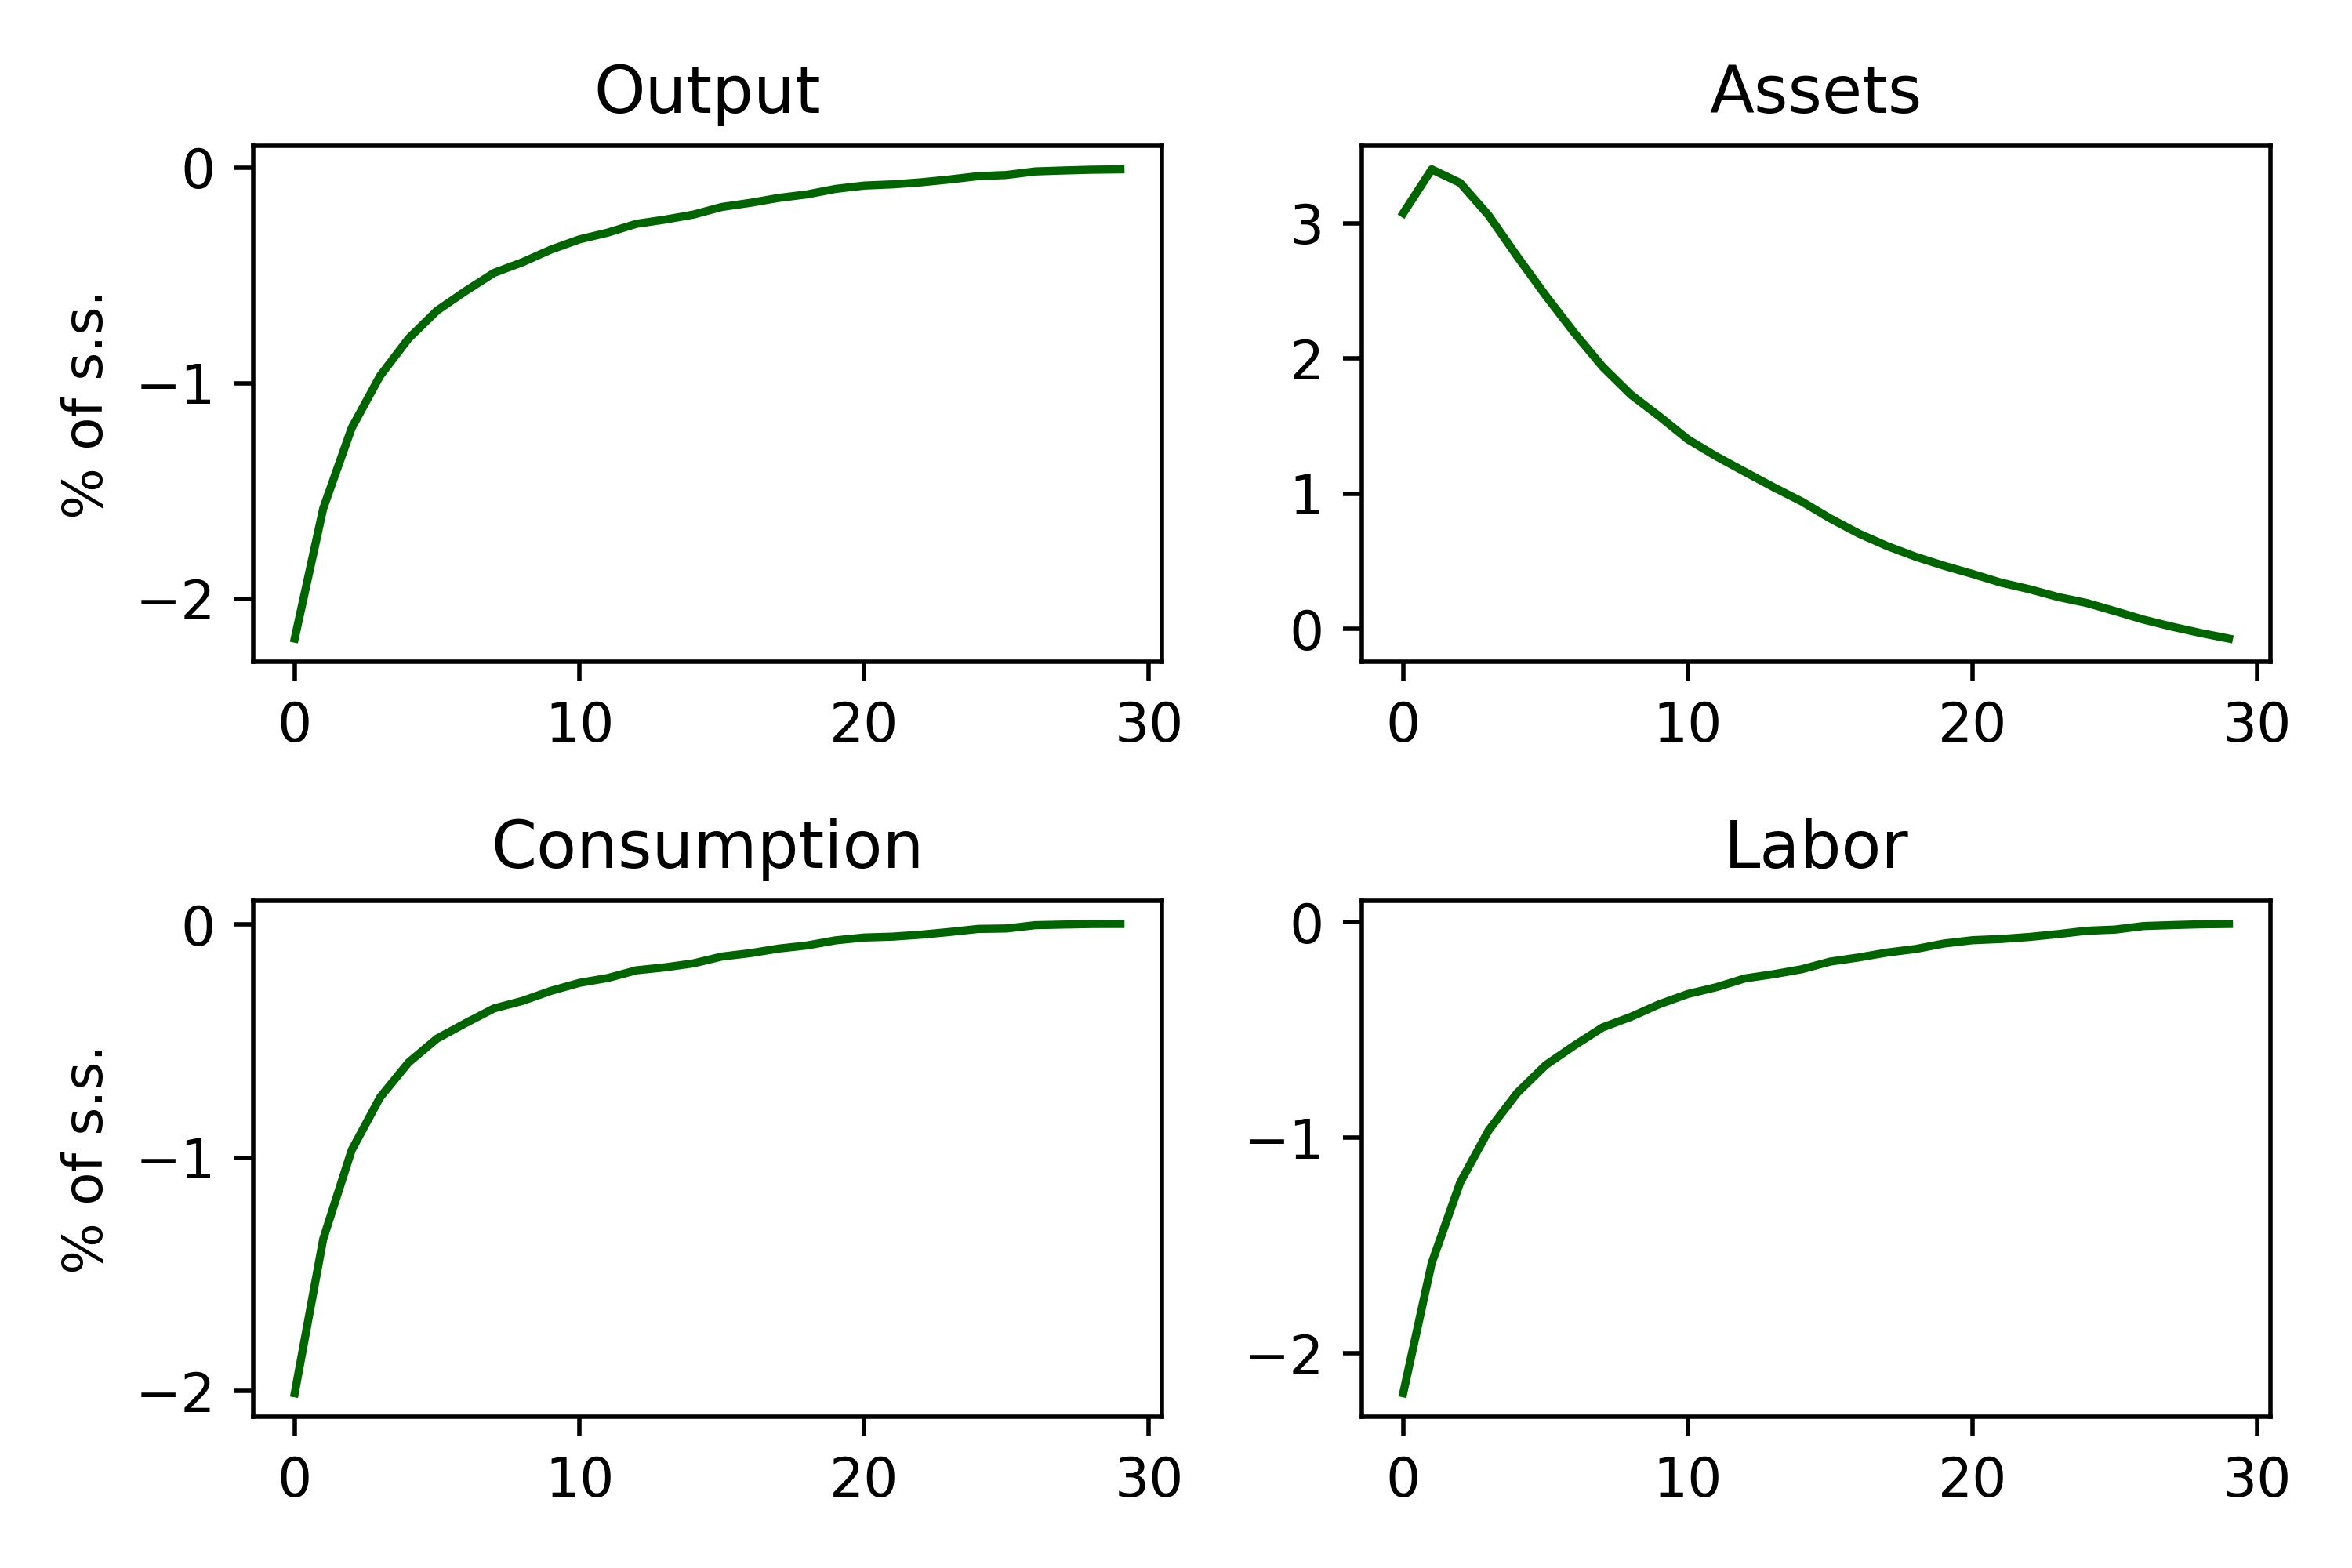
\includegraphics[scale=.35]{\FigDir/GIPRM2}
  \end{subfigure}
  \begin{subfigure}{}
    \centering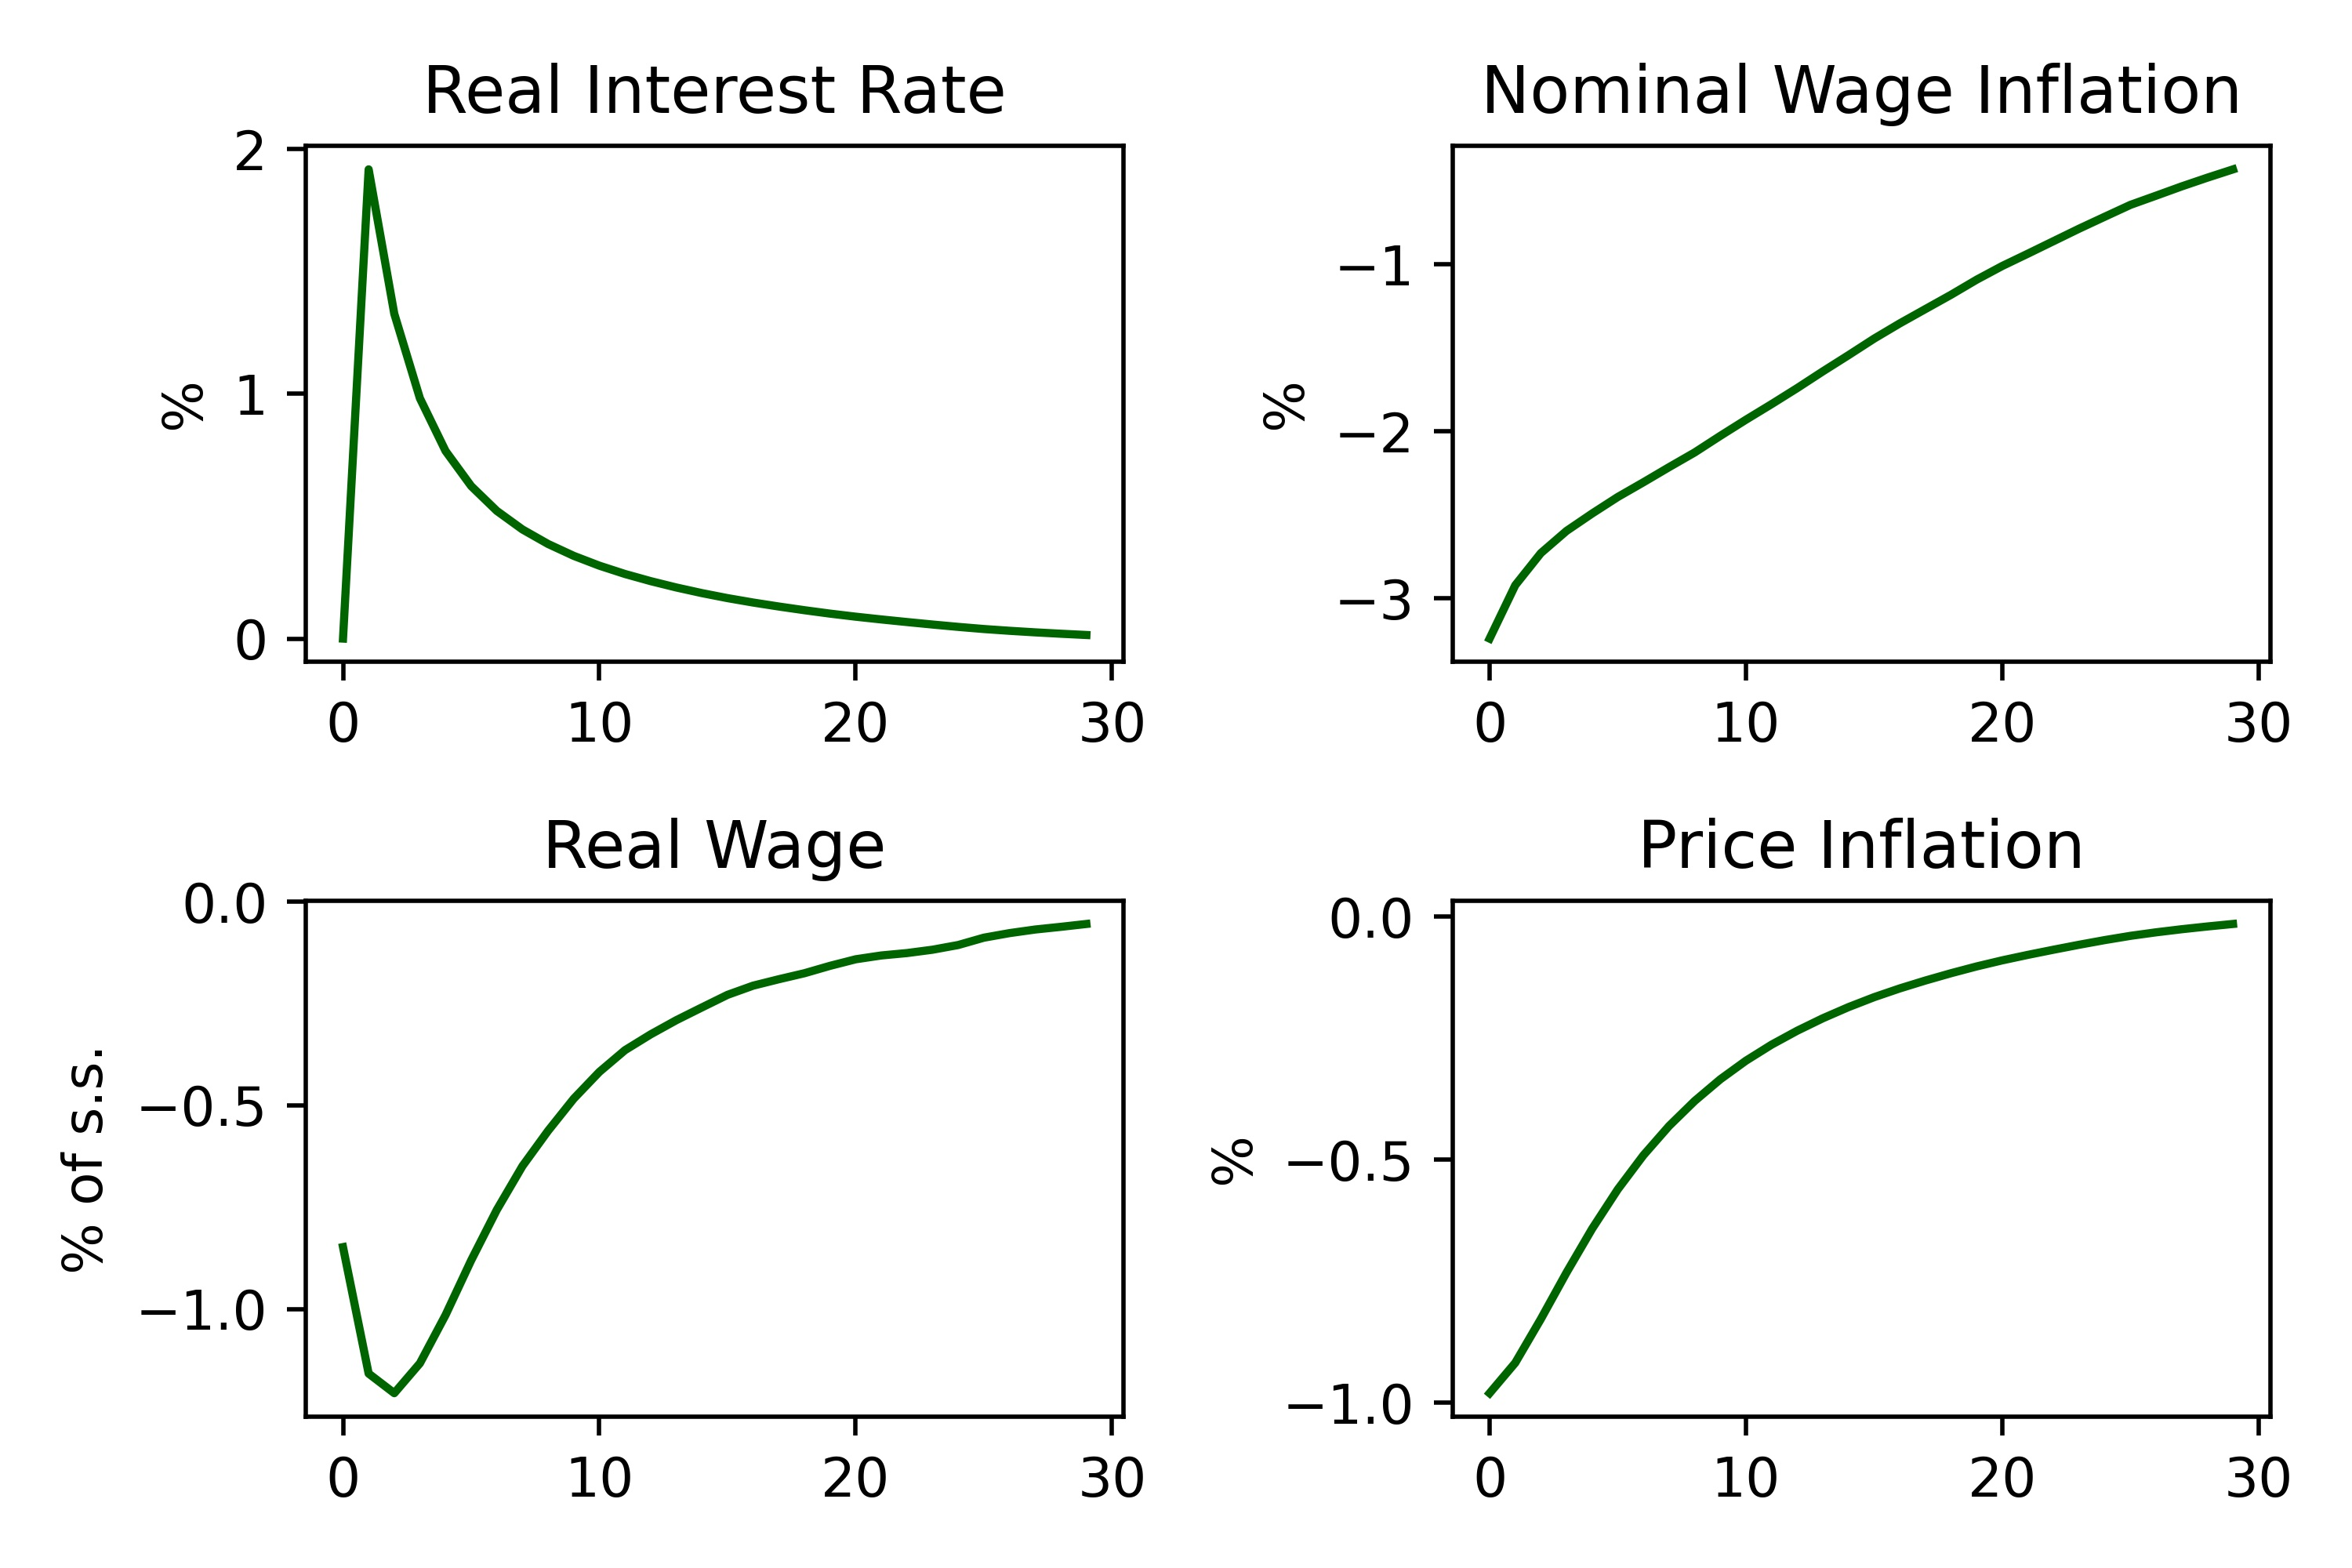
\includegraphics[scale=.35]{\FigDir/GIPRM1}
    \caption{ Impulse Response to One Percent Increase in Nominal Rate}
  \end{subfigure}
\end{figure}


\hypertarget{Productivity Shock}{}
\subsection{Productivity Shock}


The impulse responses to the productivity shock can be found in figure 2. The productivity shock is a 1 percent increase in $Z_{t}$ following an AR(1) with a coefficient of .9. The rise in productivity raises both output and firm markups, inducing downward pressure on prices which inturn induces downward pressure on nominal wages. However, given the goods market must clear, consumption must rise causing upward pressure on the nominal wage since the economy marginal rate of substitution is a function of the average marginal utility of consumption. The net effect will see nominal wages rise leading to upward pressure on prices. The net effect of all these different pressures will see the real wage rise and therefore amplify the consumption response signficantly due to the large aggregate MPC in the model. In addition, to the fixed nominal interest rate, inflation will see the real interest rate fall further amplifying consumption. This amplification of consumption will lead to rises in output and labor due to upward pressure on labor demand.

\begin{figure}{Impulse Responses to a Productivity Shock}
  \begin{subfigure}{}
    \centering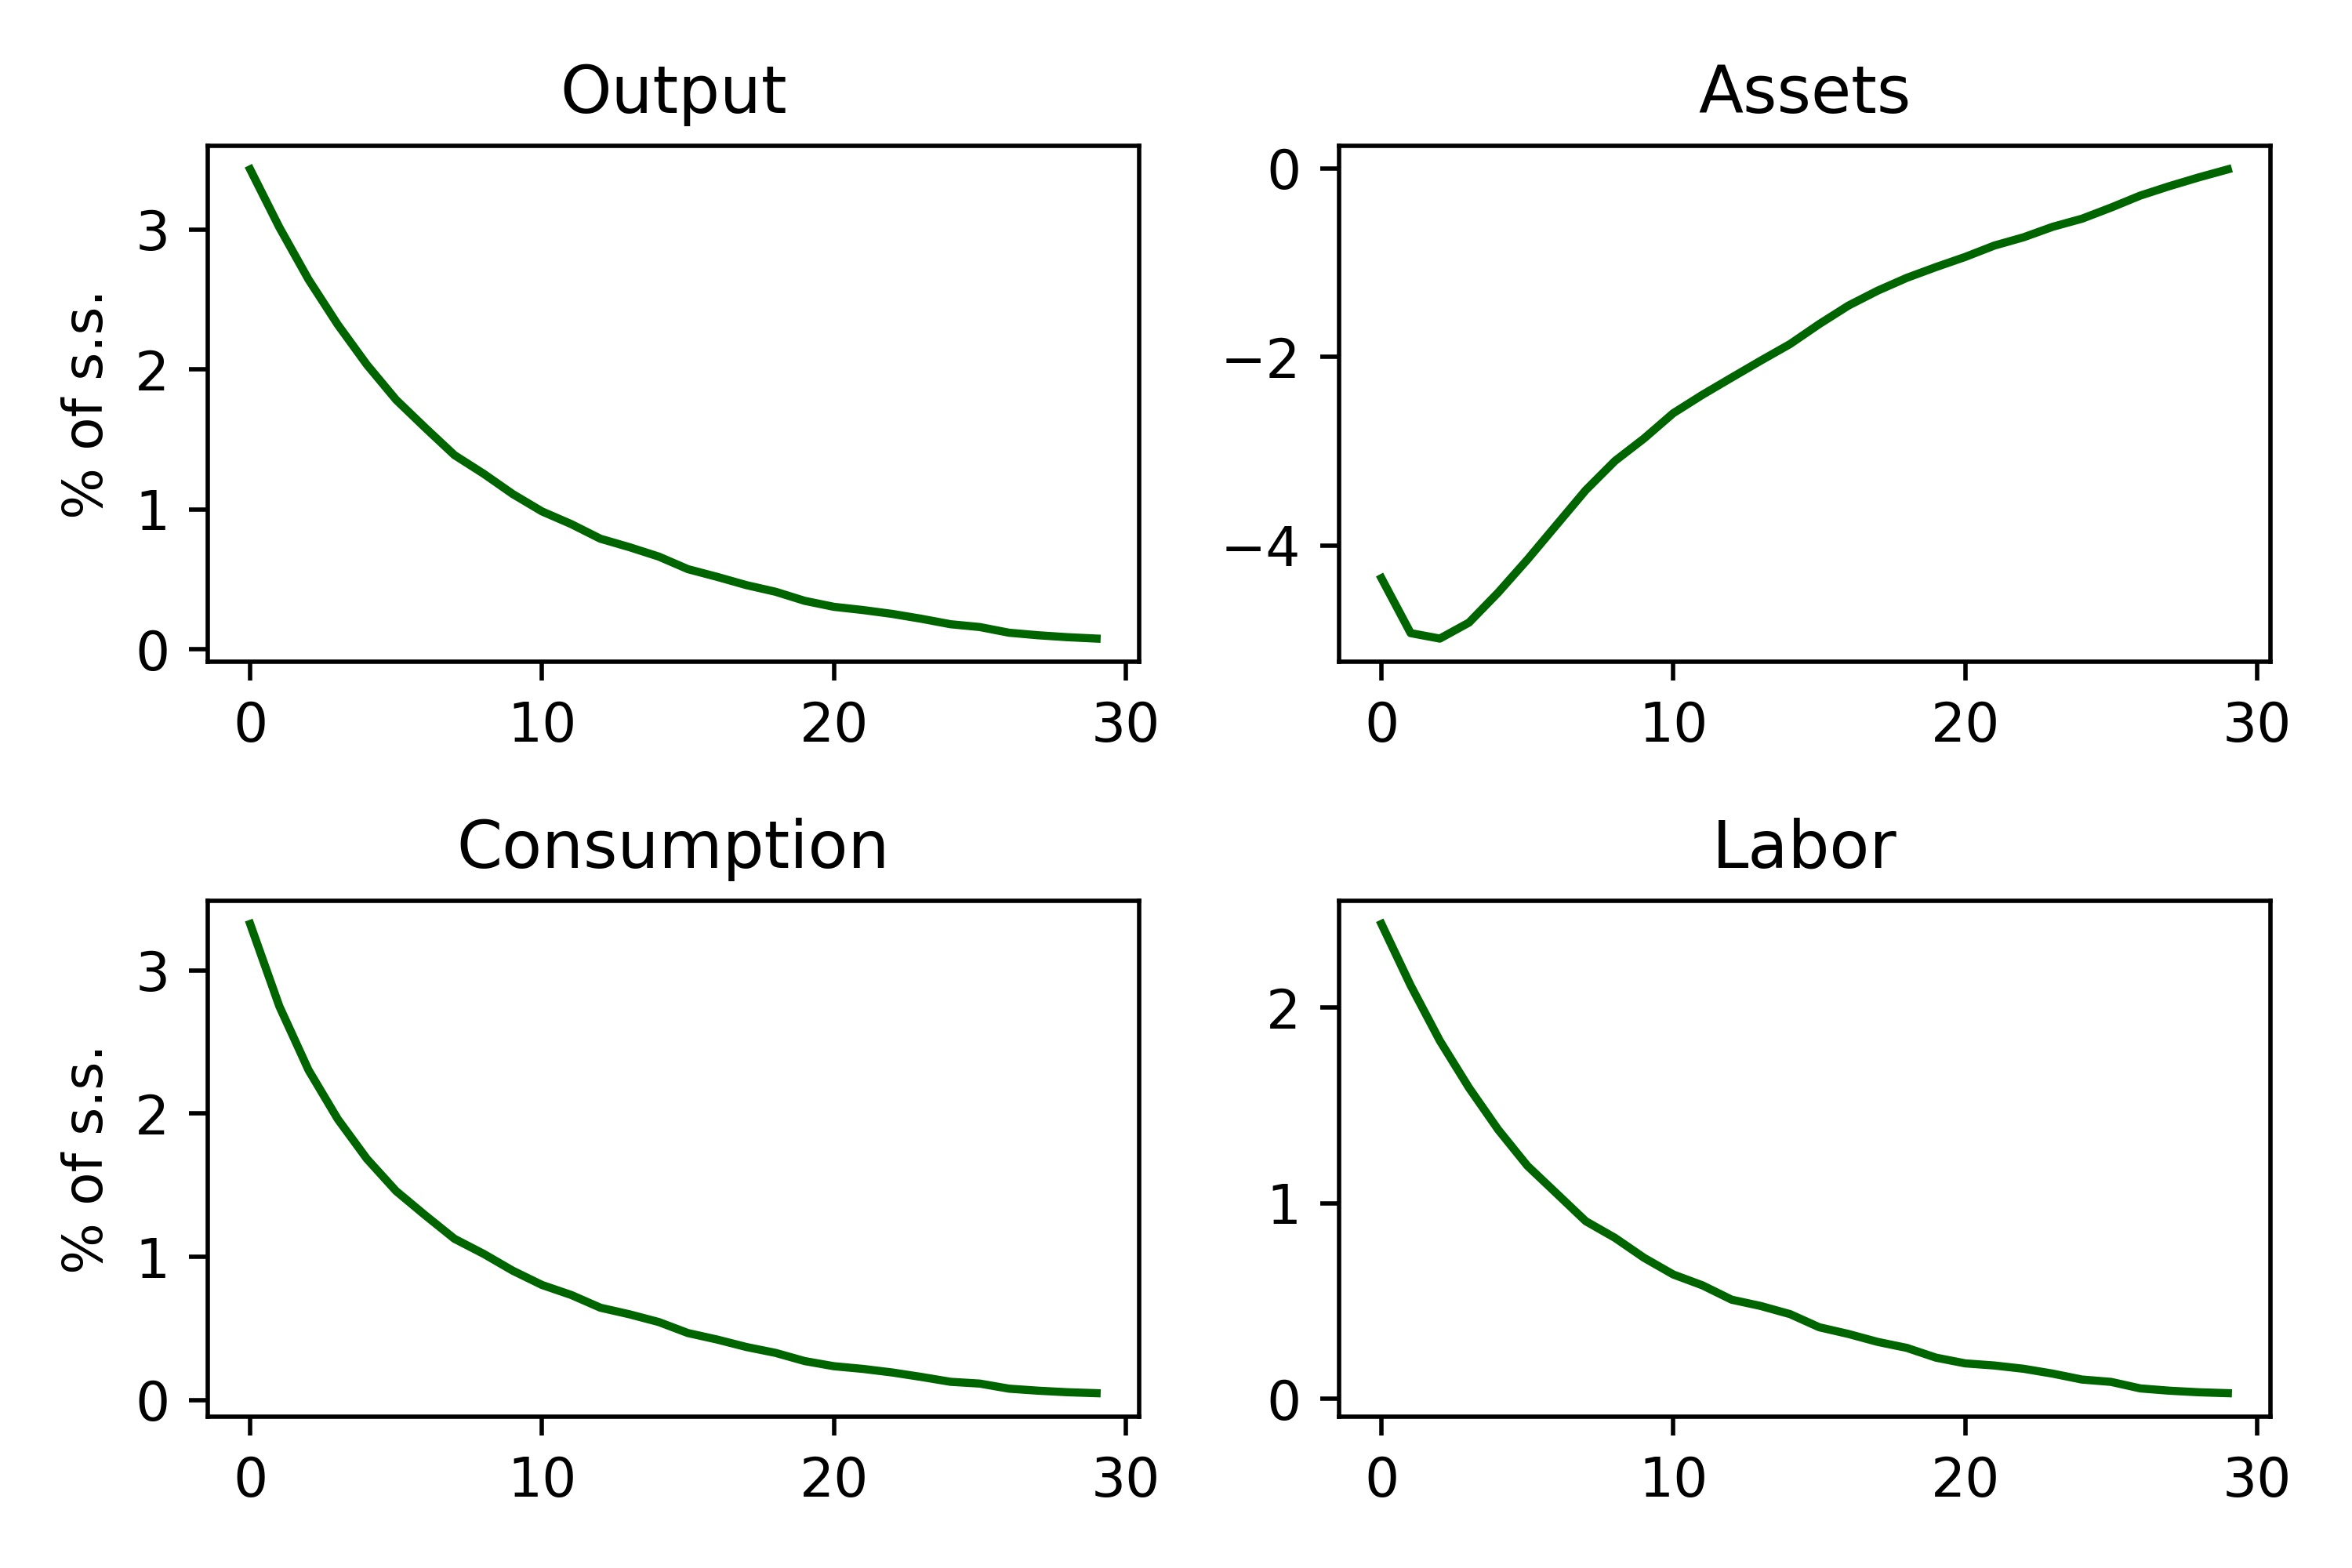
\includegraphics[scale=.35]{\FigDir/GIPRZ2}
  \end{subfigure}
  \begin{subfigure}{}
    \centering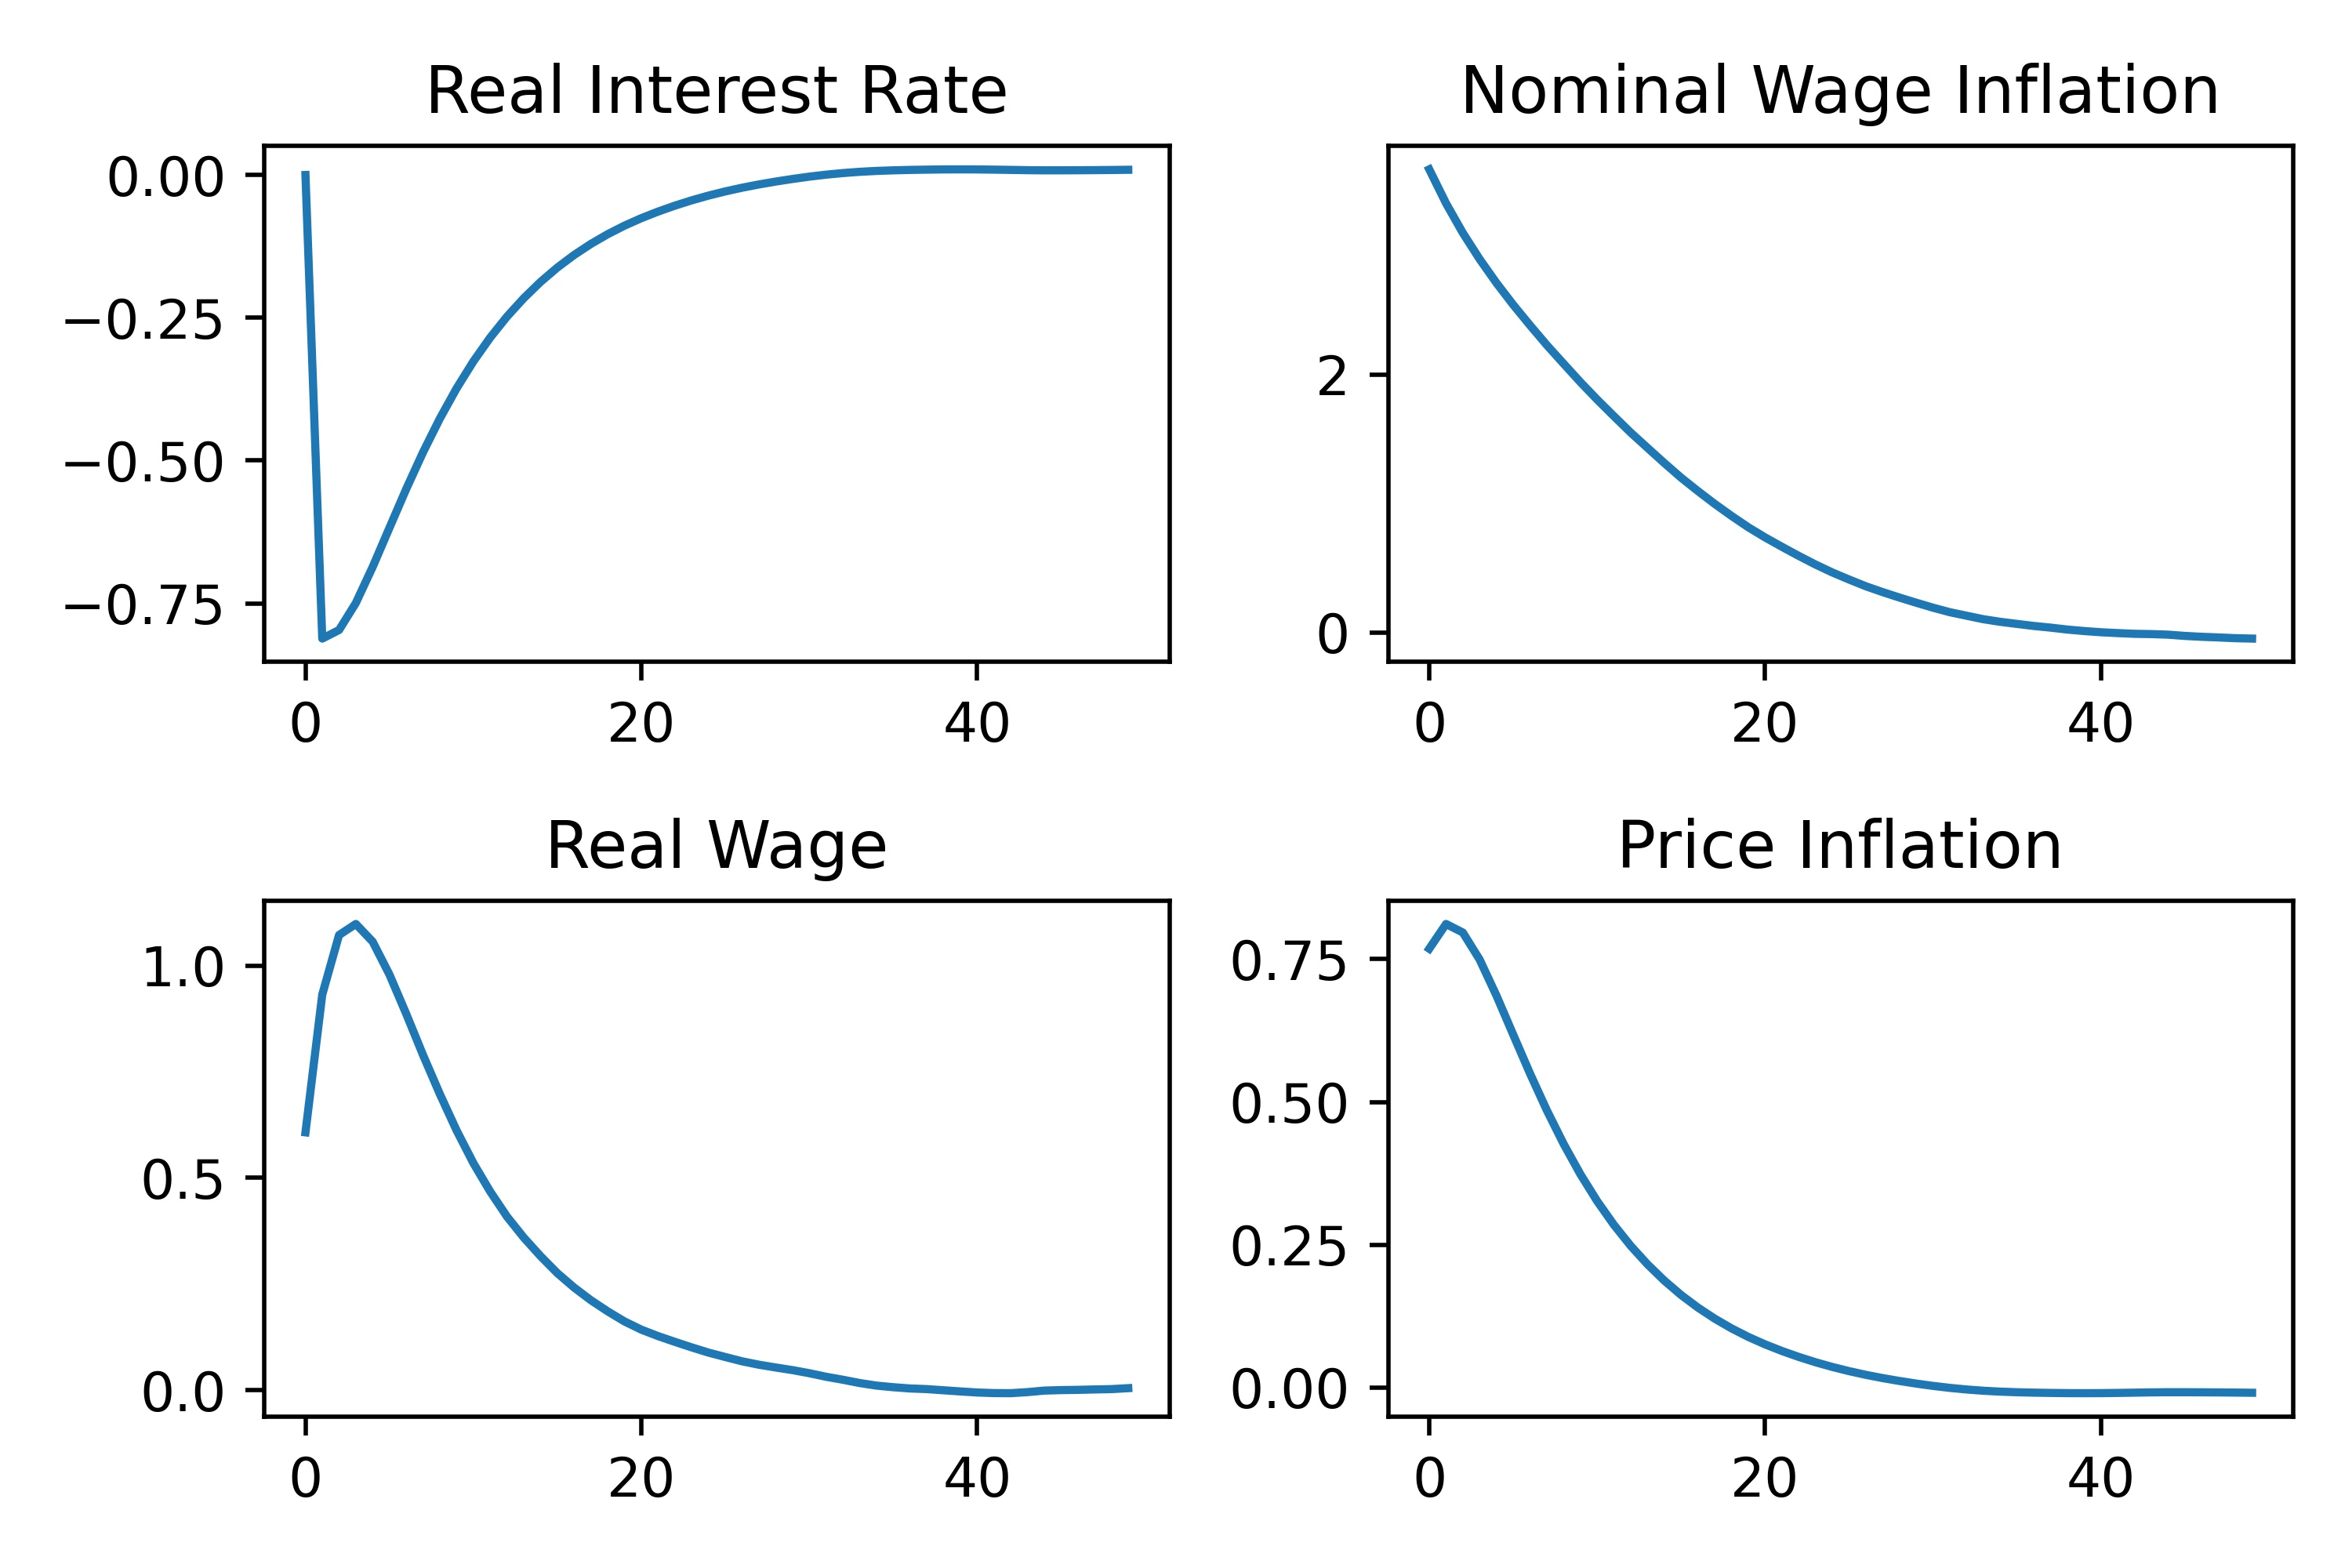
\includegraphics[scale=.35]{\FigDir/GIPRZ1}
    \caption{ Impulse Response to One Percent Increase in $Z_{t}$}
  \end{subfigure}
\end{figure}



\hypertarget{Issues and Extensions}{}
\section{Issues and Extensions}

The most prominent issue I have encountered thus far is determining whether the impulse responses are accurate in regards to the specification of the model. Producing the impulses responses is an exercise in linear algebra and the computation of jacobians. Because the jacobians were constructed without automatic differentiation, the accuracy of the impulse responses produced is uncertain as the smallest algebraic mistake may render them incorrect. Despite this uncertainty, the impulse responses of the model do mirror the responses produced from dynare under certain calibrations.  In particular, as long as prices are calibrated to be slightly stickier than wages, the impulse responses from a monetary policy shock behave in exactly the same manner as those produced from dynare. In addition, the impulse responses from a productivity shock seem essentially no different to those produced from dynare. The only issue is whenever wages are calibrated to be stickier than prices. When wages are stickier than prices,  to be specific, if the parameter for wage stickiness is set to .85 and the that of price stickiness to .8, the impulse responses to a monetary contraction are quantitatively the same as those seen in section 5 except they all invert across the x axis. That is, with the rise in the nominal rate, the results see a rise in consumption, output, labor, inflation and the real wage. This is much cause for concern regarding the accuracy of the code that produces the impulse responses as they do not survive under calibrations where wages are stickier than prices. It is possible, however, that these inverted responses may be accurate to the model due to the strong responsiveness of consumption present in the model. For instance, when the inverse frish elasticity is set to a large value (from v =2 to v=7) rendering labor to be significantly less sensitive to changes in wages, the impulse responses do not invert anymore ( consumption, output, labor, real wages all fall after a rise in the nominal rate). This is evidence that perhaps the consumption response is so strong that the slightest change in calibration could lead to large amplification effects that can invert the impulse response. My current hypothesis is that when prices are slightly more flexible than wages, the real wage may perhaps rise as since an increase in the nominal rate induces downward pressure on both prices and wages and if the fall in prices is larger than the fall in wages, the real wage may rise inducing a strong consumption response which amplifies and lead aggregate variables such as labor supply, and output to rise when the real rate rises. 
























%\providecommand{\figName}{GIPRM1}
%\providecommand{\figFile}{GIPRM1}
%\hypertarget{\figFile}{}
%\hypertarget{\figName}{}
%\begin{figure}[tbp]
%\centerline{\includegraphics[scale=.35]{\FigDir/\figFile}}
%\caption{Monetary Policy Shock}
%\label{fig:\figFile}
%\end{figure}


%%
%\renewcommand{\figFile}{GIPRM2}
%\hypertarget{\figFile}{}  
%\begin{figure}[tbp]
%\centerline{\includegraphics[scale=.35]{\FigDir/\figFile}}
%\caption{Monetary Policy Shock}
%\label{fig:\figFile}
%\end{figure}
%%


\clearpage\vfill\eject

\appendix

\centerline{\LARGE Appendices}\vspace{0.2in}




\hypertarget{Computational Details}{}
\section{Computational Details}

\hypertarget{Household Bellman Equation }{}
\subsection{Household Bellman Equation}

Household i's dynamic program is

$$ V(\pmb{\mathrm{m}}_{it},\pmb{\mathrm{p}}_{it})=\max_{ \{ \pmb{\mathrm{c}}_{it}\}} { \frac{\cLevBF_{i t}^{1-\rho}}{1 -\rho} - \varphi \pLevBF_{it} \frac{n_{it}^{1+v}}{1+v} + \beta_{i} \not D \mathrm{E}_{t}[V( \pmb{\mathrm{m}}_{it+1} , \pmb{\mathrm{p}}_{it+1})]}$$

subject to 

\begin{align*}
 \pmb{\mathrm{m}}_{i t} & = \pmb{\mathrm{z}}_{i t}  + (1+\mathit{r}^{a}_{t})\pmb{\mathrm{a}}_{i t-1} \\
 \pmb{\mathrm{c}}_{i t}  + \pmb{\mathrm{a}}_{i t} &= \pmb{\mathrm{z}}_{i t}  + (1+\mathit{r}^{a}_{t}) \pmb{\mathrm{a}}_{i t-1}   \\
\pmb{\mathrm{a}}_{it} &\geq 0 
\end{align*} \\ \\

This can be normalized to \\


$$ V(m_{it}) = \max_{\{c_{it}\}} {  \frac{c_{i t}^{1-\rho}}{1 -\rho} - \varphi \frac{n_{it}^{1+v}}{1+v} + \beta_{i}\not D \mathrm{E}_{t}[\psi_{it+1}^{1-\rho} V(m_{it+1})]}$$

 subject to 
 
 \begin{align*}
m_{i t} &=  \xi_{it}  + (1+r^{a}_{t}) \frac{a_{i t-1}}{\psi_{it}} \\
 c_{i t}  + a_{i t} &= \xi_{it}  + (1+r^{a}_{t}) \frac{a_{i t-1}}{\psi_{it}} \\
 a_{it} &\geq 0 
 \end{align*}
 
 Here non boldface variables are normalized by permanent income $\mathit{p_{it}}$. 

e.g. $x_{it} = \frac{\mathbf{x_{it}}}{\pmb{\mathrm{p}}_{it}}$ \\

First order condition for consumption:

$$c_{it}^{-\rho} -  \beta_{i} \not D \mathrm{E}_{t}\left[ (1+r^{a}_{t+1})  \psi_{it+1}^{-\rho} V'(m_{it+1})\right] = 0$$ \\ 



%%Now let $v(m_{it}, c_{it}) = \frac{c_{i t}^{1-\rho}}{1 -\rho} - \varphi \frac{n_{it}^{1+v}}{1+v} + \beta_{i}\not D \mathrm{E}_{t}[\psi_{it+1}^{1-\rho} V(m_{it+1})] $ and let $c_{it}(m_{it})$ denote the solution to the original dynamic problem.  \\ 

%%Note $ \frac{ \partial v(m_{it},c_{it}(m_{it}))}{\partial m} =  \beta_{i}\not D \mathrm{E}_{t}[\psi_{it+1}^{1-\rho} V'(m_{it+1})] $ \\

%%Then $$ V(m_{it}) = v(m_{it}, c_{it}(m_{it})$$ 

%%$$ V'(m_{it}) = \frac{ \partial v(m_{it},c_{it}(m_{it}))}{\partial m}$$ 

%%Which leads to the envelope condition \\

%%$$V'(m_{it}) =  \beta_{i}\not D \mathrm{E}_{t}[\psi_{it+1}^{1-\rho} V'(m_{it+1})] $$




\hypertarget{Model as System}{}
\subsection{Model as System}

The model can be defined by the system of equations below. The solution of the model must see this system be equal to a vector of zeros for periods $t =0, 1, 2, 3, ...$. The system is defined over the sequence space of all endogenous variables $\mathbf{U}$  and exogenous variables $\mathbf{Z}$ of the model.

$$
H_{t}(\mathbf{U},\mathbf{Z})= \begin{pmatrix} 
 Y_{t} - Z_{t}N_{t} \\ \\ 
B_{t-1} - q^{b}_{t}B_{t} + u\mho + G - \tau w_{t} N_{t} \\ \\  
i_{t} - r^{*} - \phi \pi^{p}_{t} -\phi_{y}(Y_{t}-Y_{ss}) - v_{t} \\ \\
\pi_{t}^{p} -\frac{\pi^{p}_{t+1}}{1+r^{*}} + \lambda(\mu_{t}^{p} -\mu_{p})  \\ \\
 \pi_{t}^{w} -\not D \pi_{t+1}^{w} -(\frac{1-\lambda_{w}}{\lambda_{w}}) (1- \not D \lambda_{w}) (\mu^{w} -\mu_{t}^{w}) \\ \\
    1+r_{t} - \frac{1 + i_{t}}{1+ \pi^{p}_{t+1}}\\ \\
 1+r_{t+1}^{a} - \frac{q_{t+1}^{s} +D_{t+1}}{q_{t}^{s}} \\ \\
 r_{t} - r_{t+1}^{a} \\ \\
 \frac{w_{t}}{w_{t-1}} - \frac{\Pi_{t}^{w}}{\Pi_{t}^{p}} \\ \\
 \mathcal{C}_{t}(\{r_{s}^{a} ,w_{s}, N_{s}\}_{s=0}^{s=T}) - Y_{t} + G \\ \\
 \end{pmatrix} = \begin{pmatrix} 0 \\ 0 \\. \\. \\. \\ 0\\ \end{pmatrix} , \quad t=0,1 ,2,3,....
$$ \\ \\
 

 
 where \\
 
$\mathcal{C}_{t}(\{r_{s}^{a} ,w_{s}, N_{s}\}_{s=0}^{s=T}) = \int_{0}^{1} \pLevBF_{it} c_{it}(m_{it})\, di $ \\
 
$c_{it}(m_{it})$ is the steady state normalized consumption policy for household $i$ in period t. \\ \\
 

 
 
 $\mathbf{U} = \left(Y_{t} , N_{t} ,  D_{t
 }, B_{t}, w_{t} , \pi_{t}^{p} ,\pi_{t}^{w}, r_{t} , r_{t+1}^{a}, i_{t} , q_{t}^{s},  q_{t}^{s} \right)_{t=0}^{t=T}$ \\ 

 
 $\mathbf{Z} = \left(Z_{t} ,v_{t}\right)_{t=0}^{t=T}$ \\
 
 \textbf{Note} the asset market clearing condition is not included in the system as the goods market clearing condition holds if and only if the asset market clearing condition holds. On the same note, the government budget constraint nor the equation for the stock price is included in the reduced system as they both bonds and its stock price appears in the asset clearing equation.  \\ \\
 
 
 
\hypertarget{Reduced System}{}
\subsubsection{Reduced System}
 
The previous system of a little more than a dozen endogenous variables can be reduced to a system of three endogenous variables. \\ 
 
Endogenous Variables are $ r_{t} , w_{t} ,N_{t}$ \\ 
 
Exogenous Variables are $ Z_{t}, v_{t}$ \\ 

The reduced system: \\ \\

\begin{eqnarray} 
H_{t}(\mathbf{U},\mathbf{Z})= \begin{pmatrix} 
\mathcal{H}_{t,1} \\ \\ 
\mathcal{H}_{t,2} \\ \\
\mathcal{H}_{t,3} \\ \\
 \end{pmatrix} = \begin{pmatrix} 0 \\ 0 \\ 0 \\ \end{pmatrix} , \quad  t = 0, 1, 2, ..., T 
 \end{eqnarray}
 
 where \\ 
 
 
 $\mathcal{H}_{t,1}  =\mathcal{C}_{t}\left( \left \{r^{a}_{s} , w_{s} , N_{s}  \right \}_{s=0}^{s=T} \right) - Z_{t} N_{t} + G\\ \\ $

$ \mathcal{H}_{t,2}  =log(w_{t}) - log(w_{t-1}) + \left( \frac{1 - \lambda_{w}}{\lambda_{w}}(1 - \not D \lambda_{w}) \sum_{k=0}^{\infty} \not D^{k} ( \mu_{t+k}^{w} - \mu^{w}) \right) - \left(  \lambda \sum_{k=0}^{\infty} \frac{1}{(1+r^{*})^{k}} ( \mu_{t+k}^{p} - \mu^{p})\right)\\ \\ $

$ \mathcal{H}_{t,3}  =  (1+r_{t}) \left(1+ -\lambda \sum_{k=1}^{\infty} \frac{1}{(1+r^{*})^{k}} ( \mu_{t+k}^{p} - \mu^{p}) \right) \\ \\
 - \left(1+r^{*}+ \phi \left(- \lambda \sum_{k=0}^{\infty} \frac{1}{(1+r^{*})^{k}} ( \mu_{t+k}^{p} - \mu^{p}) \right) +\phi_{y} \left(Z_{t} N_{t} - Y_{ss} \right) + v_{t}\right) \\ \\ $
 
$ \mu_{t}^{p} = log(\frac{1}{w_{t}}) + log(Z_{t})$ \\ 

$\mu_{t}^{w} = log(w_{t}) + log(1 - \tau_{t}) - mrs_{t} \\  $

$mrs_{t} = log \left(- \frac{\int_{0}^{1}   U_{n} \left(\cLevBF_{i t}, n_{i t} \right) \ d i  }{\int_{0}^{1} \pLevBF_{it} \theta_{it} U_{c} \left(\cLevBF_{i t}, n_{i t} \right) \  di } \right) = log \left(\frac{\int_{0}^{1} \varphi \pLevBF_{it} n_{it}^{v} \ d i  }{\int_{0}^{1} \pLevBF_{it}  \theta_{it} \cLevBF_{it}^{-\rho} \  di } \right) = log \left(\frac{\int_{0}^{1} \varphi \pLevBF_{it} \left(\frac{N_{t}}{1 - \mho} \right)^{v} \, d i  }{\int_{0}^{1} \pLevBF_{it}  \theta_{it} \cLevBF_{it}^{-\rho} \  di } \right)$ \\ 

$ = log \left( \varphi \left(\frac{N_{t}}{1 - \mho}\right) ^{v}\right) + log \left(\int_{0}^{1} \pLevBF_{it}  \,  di  \right) - log \left(\int_{0}^{1} \pLevBF_{it}  \theta_{it} \cLevBF_{it}^{-\rho} \  di  \right) $ \\ \\
 
 and the arguments of the function $H_{t}$ are \\
 
$\mathbf{U} = (r_{0} , r_{1} , ...r_{T}, w_{0}, w_{1}, ..., w_{T}, N_{0}, N_{1},...,N_{T})$ \\ 

$ \mathbf{Z} = ( Z_{0}, Z_{1},... Z_{T}, v_{0},...,v_{T}) \\ \\ $ 




\hypertarget{Jacobian of System}{}
\subsection{Jacobian of System} 

\hypertarget{Implicit Function Theorem}{}
\subsubsection{Implicit Function Theorem} 

By applying the implicit function theorem to the reduced system, we can obtain the endogenous responses of the real interest rate, wage, and labor supply given some exogenous shock \\

$$d\mathbf{U} =  -{\mathbf{H}_{\mathbf{U}}}^{-1} \mathbf{H}_{\mathbf{Z}} d \mathbf{Z}$$ \\ 

where $d\mathbf{U}$ are the endogenous responses of the real interest rate, the real wage, and labor supply to an exogenous shock $d \mathbf{Z}$.

Specifically, notation is defined below\\


$$d\mathbf{U} =(dr_{0} , dr_{1} , ...dr_{T}, dw_{0}, dw_{1}, ..., dw_{T}, dN_{0}, dN_{1},...,dN_{T})$$

$$d \mathbf{Z} = ( dZ_{0}, dZ_{1},... dZ_{T}, dv_{0},...dv_{T}) $$ \\





 $$  \mathbf{H}_{\mathbf{U}}= \begin{pmatrix} 
H_{\mathbf{U}, 1} \\ \\ 
H_{\mathbf{U}, 2}  \\ \\
H_{\mathbf{U}, 3} \\ \\
 \end{pmatrix} \quad \quad \mathbf{H}_{\mathbf{Z}}= \begin{pmatrix} 
H_{\mathbf{Z}, 1} \\ \\ 
H_{\mathbf{Z}, 2}  \\ \\
H_{\mathbf{Z}, 3} \\ \\
 \end{pmatrix}$$ \\ \\
 
 
 $$ H_{\mathbf{U}, i}= \begin{pmatrix} 
\frac{ \partial \mathcal{H}_{0,i}}{\partial r_{0}}  & ... & \frac{ \partial \mathcal{H}_{0,i}}{\partial r_{T}} & \frac{ \partial \mathcal{H}_{0,i}}{\partial w_{0}} & ... & \frac{ \partial \mathcal{H}_{0,i}}{\partial w_{T}} & \frac{ \partial \mathcal{H}_{0,i}}{\partial N_{0}} & ... &\frac{ \partial \mathcal{H}_{0,i}}{\partial N_{T}} \\ \\ 
\frac{ \partial \mathcal{H}_{1,i}}{\partial r_{0}}  & ... & \frac{ \partial \mathcal{H}_{1,i}}{\partial r_{T}} & \frac{ \partial \mathcal{H}_{1,i}}{\partial w_{0}} & ... & \frac{ \partial \mathcal{H}_{1,i}}{\partial w_{T}} & \frac{ \partial \mathcal{H}_{1,i}}{\partial N_{0}} & ... &\frac{ \partial \mathcal{H}_{1,i}}{\partial N_{T}}  \\ \\
.   \\ \\ \\ 
. \\ \\ \\
. \\ \\ \\
\frac{ \partial \mathcal{H}_{T,i}}{\partial r_{0}}  & ... & \frac{ \partial \mathcal{H}_{T,i}}{\partial r_{T}} & \frac{ \partial \mathcal{H}_{T,i}}{\partial w_{0}} & ... & \frac{ \partial \mathcal{H}_{T,i}}{\partial w_{T}} & \frac{ \partial \mathcal{H}_{T,i}}{\partial N_{0}} & ... &\frac{ \partial \mathcal{H}_{T,i}}{\partial N_{T}} \\ \\
 \end{pmatrix} $$ \\
 
  $$ H_{\mathbf{Z}, t}= \begin{pmatrix} 
\frac{ \partial \mathcal{H}_{0,i}}{\partial Z_{0}}  & ... & \frac{ \partial \mathcal{H}_{0,i}}{\partial Z_{T}} & \frac{ \partial \mathcal{H}_{0,i}}{\partial v_{0}} & ... & \frac{ \partial \mathcal{H}_{0,i}}{\partial v_{T}} \\ \\ 
\frac{ \partial \mathcal{H}_{1,i}}{\partial Z_{0}}  & ... & \frac{ \partial \mathcal{H}_{1,i}}{\partial Z_{T}} & \frac{ \partial \mathcal{H}_{1,i}}{\partial v_{0}} & ... & \frac{ \partial \mathcal{H}_{1,i}}{\partial v_{T}} \\ \\
. \\ \\ \\ 
. \\ \\ \\
. \\ \\ \\
\frac{ \partial \mathcal{H}_{T,i}}{\partial Z_{0}}  & ... & \frac{ \partial \mathcal{H}_{T,i}}{\partial Z_{T}} & \frac{ \partial \mathcal{H}_{T,i}}{\partial v_{0}} & ... & \frac{ \partial \mathcal{H}_{T,i}}{\partial v_{T}}  \\ \\
 \end{pmatrix} $$ \\ \\
 
 
\textbf{ Or equivalently}

 $$  \mathbf{H}_{\mathbf{U}}= \begin{pmatrix} 
H_{\mathbf{U}, 0} \\ \\ 
H_{\mathbf{U}, 1}  \\ \\
. \\ \\
. \\ \\
. \\ \\ 
H_{\mathbf{U}, T} \\ \\
 \end{pmatrix} \quad \quad \mathbf{H}_{\mathbf{Z}}= \begin{pmatrix} 
H_{\mathbf{Z}, 0} \\ \\ 
H_{\mathbf{Z}, 1}  \\ \\
. \\ \\
. \\ \\
. \\ \\ 
H_{\mathbf{Z}, T} \\ \\
 \end{pmatrix}$$ \\ \\
 
 
 
$$ H_{\mathbf{U}, t}= \begin{pmatrix} 
\frac{ \partial \mathcal{H}_{t,1}}{\partial r_{0}}  & ... & \frac{ \partial \mathcal{H}_{t,1}}{\partial r_{T}} & \frac{ \partial \mathcal{H}_{t,1}}{\partial w_{0}} & ... & \frac{ \partial \mathcal{H}_{t,1}}{\partial w_{T}} & \frac{ \partial \mathcal{H}_{t,1}}{\partial N_{0}} & ... &\frac{ \partial \mathcal{H}_{t,1}}{\partial N_{T}} \\ \\ 
\frac{ \partial \mathcal{H}_{t,2}}{\partial r_{0}}  & ... & \frac{ \partial \mathcal{H}_{t,2}}{\partial r_{T}} & \frac{ \partial \mathcal{H}_{t,2}}{\partial w_{0}} & ... & \frac{ \partial \mathcal{H}_{t,2}}{\partial w_{T}} & \frac{ \partial \mathcal{H}_{t,2}}{\partial N_{0}} & ... &\frac{ \partial \mathcal{H}_{t,2}}{\partial N_{T}}  \\ \\
\frac{ \partial \mathcal{H}_{t,3}}{\partial r_{0}}  & ... & \frac{ \partial \mathcal{H}_{t,3}}{\partial r_{T}} & \frac{ \partial \mathcal{H}_{t,3}}{\partial w_{0}} & ... & \frac{ \partial \mathcal{H}_{t,3}}{\partial w_{T}} & \frac{ \partial \mathcal{H}_{t,3}}{\partial N_{0}} & ... &\frac{ \partial \mathcal{H}_{t,3}}{\partial N_{T}} \\ \\
 \end{pmatrix} $$ \\
 
  $$ H_{\mathbf{Z}, t}= \begin{pmatrix} 
\frac{ \partial \mathcal{H}_{t,1}}{\partial Z_{0}}  & ... & \frac{ \partial \mathcal{H}_{t,1}}{\partial Z_{T}} & \frac{ \partial \mathcal{H}_{t,1}}{\partial v_{0}} & ... & \frac{ \partial \mathcal{H}_{t,1}}{\partial v_{T}} \\ \\ 
\frac{ \partial \mathcal{H}_{t,2}}{\partial Z_{0}}  & ... & \frac{ \partial \mathcal{H}_{t,2}}{\partial Z_{T}} & \frac{ \partial \mathcal{H}_{t,2}}{\partial v_{0}} & ... & \frac{ \partial \mathcal{H}_{t,2}}{\partial v_{T}} \\ \\
\frac{ \partial \mathcal{H}_{t,3}}{\partial Z_{0}}  & ... & \frac{ \partial \mathcal{H}_{t,3}}{\partial Z_{T}} & \frac{ \partial \mathcal{H}_{t,3}}{\partial v_{0}} & ... & \frac{ \partial \mathcal{H}_{t,3}}{\partial v_{T}}  \\ \\
 \end{pmatrix} $$ \\ \\
 
 
 
 
\hypertarget{Obtaining All Other Responses}{}
\subsubsection{Obtaining All Other Responses} 

To obtain all other responses given the endogenous response $\mathbf{dU}$, we compute the jacobians of the endogenous variable with respect to the relevant endogenous variables that have already been solved for.  For example, to compute the response of consumption to some exogenous shock $d\mathbf{Z}$, we sum  the jacobians of consumption with respect to the real interest rate, the wage and labor supply 

$$ d\mathbf{C} = \mathcal{J}^{\mathcal{C} , r} d\mathbf{r} +\mathcal{J}^{\mathcal{C} , w} d\mathbf{w} +\mathcal{J}^{\mathcal{C} , N} d\mathbf{N} $$\\
 
 where $\mathcal{J}^{\mathcal{C} , w} $ is the jacobian of aggregate consumption  $\mathcal{C}_{t}(\{r_{s}^{a} ,w_{s}, N_{s}\}_{s=0}^{s=T}) $  with respect to the wage. \\
 
 To be clear , 
 
$$d\mathbf{w} =  ( dw_{1}, dw_{2}, . . . , dw_{T})' $$
 
 
 
 $$\mathcal{J}^{\mathcal{C} , w} =   \begin{pmatrix} 
\frac{ \partial \mathcal{C}_{0}(\{r_{s}^{a} ,w_{s}, N_{s}\}_{s=0}^{s=T})}{\partial w_{0}}  & \frac{ \partial \mathcal{C}_{0}(\{r_{s}^{a} ,w_{s}, N_{s}\}_{s=0}^{s=T})}{\partial w_{1}}&    ... & \frac{ \partial \mathcal{C}_{0}(\{r_{s}^{a} ,w_{s}, N_{s}\}_{s=0}^{s=T})}{\partial w_{T}} \\ \\ 
\frac{ \partial \mathcal{C}_{1}(\{r_{s}^{a} ,w_{s}, N_{s}\}_{s=0}^{s=T})}{\partial w_{0}}  &\frac{ \partial \mathcal{C}_{1}(\{r_{s}^{a} ,w_{s}, N_{s}\}_{s=0}^{s=T})}{\partial w_{1}}& ... & \frac{ \partial \mathcal{C}_{1}(\{r_{s}^{a} ,w_{s}, N_{s}\}_{s=0}^{s=T})}{\partial w_{T}} \\ \\
.  \\ \\
.  \\ \\
. \\ \\
\frac{ \partial \mathcal{C}_{T}(\{r_{s}^{a} ,w_{s}, N_{s}\}_{s=0}^{s=T})}{\partial w_{0}}  &\frac{ \partial \mathcal{C}_{T}(\{r_{s}^{a} ,w_{s}, N_{s}\}_{s=0}^{s=T})}{\partial w_{1}}& ... & \frac{ \partial \mathcal{C}_{T}(\{r_{s}^{a} ,w_{s}, N_{s}\}_{s=0}^{s=T})}{\partial w_{T}}  \\ \\
 \end{pmatrix} $$ \\
 
  
\hypertarget{Additional Derivations}{}
\section{Additional Derivations} 

An employed household's transitory income is \\

$$ \theta_{it}(1-\tau) \int_{0}^{1} \frac{W_{gt}}{P_{t}}n_{igt}\,dg$$

where $W_{gt}$ denotes the nominal wage for labor type $g$ and $P_{t}$ the price of the final good. \\ \\

Now noitce

$$ \theta_{it}(1-\tau) \int_{0}^{1} \frac{W_{gt}}{P_{t}}\frac{N_{gt}}{1-\mho}\,dg$$

$$ \theta_{it}(1-\tau) \int_{0}^{1} \frac{W_{gt}}{P_{t}}\frac{\left(\frac{W_{gt}}{W_{t}}\right)^{-\epsilon_{w}} N_{t}}{1-\mho}\,dg$$

$$ \theta_{it}(1-\tau) \frac{N_{t}}{(1-\mho) W_{t}^{-\epsilon_{w}}P_{t}} \int_{0}^{1}  \left(W_{gt}\right)^{1-\epsilon_{w}} \,dg $$

$$\theta_{it}(1-\tau) \frac{N_{t}}{(1-\mho) W_{t}^{-\epsilon_{w}}P_{t}} W_{t}^{1-\epsilon_{w}} $$

$$ \theta_{it}(1-\tau) \frac{W_{t}N_{t}}{(1-\mho)P_{t} }$$\\

Which leads to the expression in the paper \\

$$ \theta_{it}(1-\tau) \frac{w_{t}N_{t}}{(1-\mho)}$$

\bibliography{\econtexRoot/BufferStockTheory,economics}

Auclert et al 2020

Auclert et al 2021

Carroll 2006

CSTW(2017)

 Chetty(2012)

Reiter 2009

Simon (1956)

Theil (1957)






\end{document}


\provideboolean{Shorter}
\setboolean{Shorter}{true}
\setboolean{Shorter}{false}
\providecommand{\ShorterYN}{\ifthenelse{\boolean{Shorter}}}
\usepackage{rotating}\usepackage{subfigure}


\hypersetup{pdfauthor={William Du <wdu9@jhu.edu>},
            pdftitle={Theoretical Foundations of Buffer Stock Saving},
            pdfkeywords={Precautionary saving, buffer-stock saving, consumption, marginal propensity to consume, permanent income hypothesis},
            pdfcreator = {wdu9@jhu.edu}
}

\begin{document}\bibliographystyle{\econtexBibStyle}
\renewcommand{\onlyinsubfile}[1]{}\renewcommand{\notinsubfile}[1]{#1} 

\hfill{\tiny \texname.tex, \today}

\begin{verbatimwrite}{\texname.title}
Theoretical Foundations of Buffer Stock Saving
\end{verbatimwrite}


\title{Distribution of Wealth and Monetary Policy}

\author{William Du\authNum}

\keywords{Precautionary saving, Heterogeneous Agents, Monetary Policy, permanent income hypothesis}




\maketitle 


\hypertarget{abstract}{}
\begin{abstract}
  This paper develops a heterogenous agent new keynesian model featuring a buffer stock income process, both sticky wages and prices and heterogeneity in discount factors to generate high aggregate MPC.
\end{abstract}


\begin{authorsinfo}
\name{Contact: \href{mailto:wdu9@jhu.edu}{\texttt{wdu9@jhu.edu}}}
\end{authorsinfo}

\thanks{Thanks to }

\titlepagefinish


\newtheorem{defn}{Definition}
\newtheorem{theorem}{Theorem}

\hypertarget{Introduction}{}
\section{Introduction}

\label{sec:intro}


Write here for intro



\hypertarget{The-Model}{}
\section{The Model}

\subsection{Households}
\label{subsec:Households} 

There is a continuum of households of mass 1 distributed on the unit
interval and indexed by $i$. Households are ex-ante heterogeneous in their discount factors and subject to idiosyncratic income shocks.  Each household faces the following problem:

\begin{verbatimwrite}{\EqDir/supfn.tex}
\begin{eqnarray}
  \label{eq:supfn}
  \max_{\{\cLevBF_{it+s}\}_{s=0}^{\infty}} \mathrm{E_{t}}\left[\sum_{s=0}^{\infty} (\not D \beta_{i})^{t+s} U\left(  \cLevBF_{i t+s}, n_{i t+s}\right)\right]
\end{eqnarray}
\end{verbatimwrite}
\input{\EqDir/supfn.tex} 

subject to 
\begin{align*}
\aLevBF_{it}     &= \mLevBF_{it} - \cLevBF_{it}   \label{eq:DBCparts} \\
\aLevBF_{it} +\cLevBF_{it}    &= \mathbf{z}_{it} +   (1 + r^{a}_{t} ) \aLevBF_{it-1}   \\ 
\aLevBF_{it}  &\geq 0 \\
\end{align*}

where
$U\left(\cLevBF_{i t}, n_{i t}\right) = \frac{\cLevBF_{i t}^{1-\rho}}{1 -\rho} - \varphi \pLevBF_{it} \frac{n_{it}^{1+v}}{1+v}$  and $\beta_{i}$ is the discount factor of household $i$. $\mLevBF_{it}$ \ denotes household $i$'s market resources at time $t$ to be expended on consumption or invested at a mutual fund. $\cLevBF_{it}$ is the level of consumption of household $i$ at time $t$ and  $ \aLevBF_{it}$ is the value of household $i$'s shares at the mutual during period $t$ where the mutual fund's return is $r_{t+1}^{a}$.  $\mLevBF_{it}$ is determined by labor income,  $\mathbf{z}_{it}$, and the gross return on assets from the last period, $(1+r_{t}^{a}) \aLevBF_{it-1} $. $\not D$ is the probability of death. Death is included in our model to ensure permanent income, $\pLevBF$, and thus wealth, has a limiting distribution.   Labor supply of household $i$ at time $t$ is denoted by $n_{it}$.  Given the formulation of sticky wages described in section 2.4, labor supply is an aggregate state variable and therefore consumption serves as the sole control variable in the dynamic problem.  \\





\begin{align*}
\mathbf{z}_{it} &= \pLevBF_{it}\tShkAll_{it} \\
\pLevBF_{it+1} &=\pLevBF_{it} \pShk_{it+1} \\
\end{align*}


Labor income is subject to permanent and transitory idiosyncratic shocks. In particular, household $i$'s labor income is composed of a permanent component, $\pLevBF_{it} $ indicating the level of permanent income and a transitory component, $\tShkAll_{it} $, indicating the transitory income shock received by household $i$ at time $t$. $\pLevBF_{it} $ is subject to permanent income shocks $\pShk_{it+1}$ where $\pShk_{it}$ is iid mean one lognormal with standard deviation $\sigma_\pShk$, $\forall t$ . \\



The transitory component follows   \\
\begin{verbatimwrite}{\EqDir/tShkDef}
$$
\tShkAll _{it}=
\begin{cases}
 u \phantom{_{t+1}/\pNotZero} & \text{with probability $\mho $} \\
 \tShkEmp_{it} (1-\tau_{t})\int_{0}^{1} w_{gt}n_{igt} \, dg      & \text{with probability $1 - \mho  $} 
\end{cases} \label{eq:tShkDef}
$$
\end{verbatimwrite}
\input{\EqDir/tShkDef.tex}\\
where u is unemployment benefits, $\tau_{t}$ is the tax rate , $w_{gt}$ is the real wage for labor type $g$ at time t, $ n_{igt}$ is the labor supply for labor type $g$ and $\tShkEmp_{t}$ is an iid mean-one lognormal with standard deviation $\sigma_{\tShkEmp}$.  The probability of receiving an unemployment shock in a given period where households forego their after-tax labor income and receive unemployment benefits instead is denoted by $\mho$.  \\ \\

Given the formulation of sticky wages described in section 2.4, the transitory component simplifies to \\

\begin{equation}
\tShkAll _{it}=
\begin{cases}
 u \phantom{_{t+1}/\pNotZero} & \text{with probability $\mho $} \\
 \tShkEmp_{it} (1-\tau_{t})\frac{w_{t}N_{t}}{(1-\mho)}      & \text{with probability $1 - \mho  $} 
\end{cases} \label{eq:tShkDef}
\end{equation} 

where $w_{t}$ is the real wage and $N_{t}$  is labor supply.

For details on the derivation, see Appendix.\\ \\


\begin{comment}
Combining the transition equations, the recursive nature of
the problem allows us to rewrite it more compactly in Bellman equation form,
\begin{eqnarray*}
\VFunc_{t}(\mLevBF_{t},\pLevBF_{t}) & = & \max_{\cLevBF_{t}}~\left\{\util(\cLevBF_{t})+\DiscFac \Ex_{t}\left[ \VFunc_{t+1}((\mLevBF_{t}-\cLevBF_{t})\Rfree+ \pLevBF_{t+1}\tShkAll_{t+1},\pLevBF_{t} \PGro  \pShk_{t+1})\right]\right\}
.
\end{eqnarray*}
\end{comment} 

\hypertarget{Financial Intermediary}{}
\subsection{Financial Intermediary}

\label{subsec:Financial Intermediary}

The financial intermediary in our model performs a mutual fund activity where it  collects assets from households and invests them into government bonds $B_{t}$, stocks $v_{jt}$, and nominal reserves at the central bank $M_{t}$.\\ 

In particular, at the end of period $t$, the assets collected from households $A_{t}$ must be invested into shares $\mathit{v}_{jt}$ of firm $j$ at price  $q^{s}_{jt}$ , government bonds $B_{t}$ at price $q^{b}_{t}$ and nominal reserves $M_{t}$. 

\begin{equation} A_{t} = \frac{M_{t}}{P_{t}} +q^{b}_{t} B_{t} + \int_{0}^{1} q^{s}_{jt}\mathit{v}_{jt}\,dj \end{equation}

where $A_{t} $ is the dollar value of the mutual fund's assets at the end of period $t$ and $ \mathit{v}_{jt}$ is the portfolio share of firm $j$ stocks with $\int_{0}^{1} \mathit{v}_{jt}\,dj =1$.  \\

The mutual fund's return in the next period is then 

$$(1+r^{a}_{t+1})  = \frac{  B_{t} + \int_{0}^{1} (q^{s}_{jt+1}+ D_{jt+1})\mathit{v}_{jt} \, dj +(1+i_{t}) \frac{M_{t}}{P_{t+1}}}{A_{t}}$$\\ 

where  $D_{jt+1}$ are dividends of firm $j$ and $i_{t}$ is the nominal interest rate  on nominal reserves. \\ \\

The mutual fund is risk neutral and looks to maximize its expected return 


$$\max_{\{B_{t}, M_{t} , \mathit{v}_{jt} \}} \mathrm{E}_{t}\left[1+r^{a}_{t+1} \right] = \mathrm{E}\left[ \frac{ B_{t} + \int_{0}^{1} (q^{s}_{jt+1}+ D_{jt+1})\mathit{v}_{jt} \, dj +(1+i_{t}) \frac{M_{t}}{P_{t+1}}}{\frac{M_{t}}{P_{t}} +q^{b}_{t} B_{t} + \int_{0}^{1} q^{s}_{jt}\mathit{v}_{jt}\,dj} \right]$$ \\

 
The first order conditions lead to the no arbitrage equations:

\begin{equation} \mathrm{E}_{t}\left[1+r^{a}_{t+1}\right]= \frac{1}{q^{b}_{t}}  =\frac{\mathrm{E}_{t}\left[q^{s}_{jt+1} + D_{jt+1} \right]}{q^{s}_{jt}} = (1+i_{t}) \mathrm{E}_{t}\left[\frac{P_{t}}{P_{t+1}}\right] \equiv 1 +r_{t} \end{equation}

where $r_{t}$ is defined to be the real interest rate in period $t$. 
In equilibrium ,we will assume $M_{t} =0$ \\ \\

\hypertarget{Goods Market}{}
\subsection{Goods Market}

There is a continuum of  monopolistically competitive intermediate good producers indexed by $j \in [0,1]$ who produce intermediate goods $Y_{jt}$ to be sold to a final good producer at price $P_{jt}$. Using intermediate goods $Y_{jt}$ for $j \in [0,1]$, the  final good producer produces a final good $Y_{t}$ to be sold to households at price $P_{t}$.  \\ 


\hypertarget{Final Good Producer}{}
\subsubsection{Final Good Producer}

A perfectly competitive final good producer purchases intermediate goods $Y_{jt}$ from intermediate good producers at price $P_{jt}$ and produces a final good $Y_{t}$ according to a CES production Function. 

$$ Y_{t} = \left(\int_{0}^{1} Y_{jt}^{\frac{\epsilon_{p}-1}{\epsilon_{p}}}\, dj\right)^{\frac{\epsilon_{p}}{\epsilon_{p}-1}}$$ \\

where $\epsilon_{p}$ is the elasticity of substitution. \\ 

Given $P_{jt}$ , the price of intermediate good $j$ ,  the final good producer maximizes his profit

$$ \max_{Y_{jt}} P_{t} \left(\int_{0}^{1} Y_{jt}^{\frac{\epsilon_{p}-1}{\epsilon_{p}}}\, dj\right)^{\frac{\epsilon_{p}}{\epsilon_{p}-1}} - \int_{0}^{1} P_{jt} Y_{jt} ,\ dj $$ \\


The first order condition leads to demand for good $j$

\begin{equation} Y_{jt} = \left(\frac {P_{jt}}{P_{t}}\right)^{- \epsilon_{p}} Y_{t}\end{equation} \\

and the price index

\begin{equation} P_{t} = \left(\int_{0}^{1} P_{jt}^{1-\epsilon_{p}}\,dj \right )^{\frac{1}{1-\epsilon_{p}}} \end{equation}


\hypertarget{Intermediate Good Producer}{}
\subsubsection{Intermediate Good Producer}

Intermediate goods producers  employ labor and produce according to a Cobb Douglas Production function.  

$$Y_{jt} =  Z_{t}  N_{jt}$$ 

where $log(Z_{t}) = \rho_{Z} log( Z_{t-1}) + \epsilon_{Z}$ \\ \\


Prices are sticky a la Calvo where each period intermediate good producers may reset their price with probability $ 1 -\lambda_{p}$ . Following Auclert et al 2020., each intermediate firm $j$ chooses $P_{jt}$ to maximize its dividend $D_{jt}$ and  stock price $q^{s}_{jt} $ \\ 
 
 $$\max_{\{P_{jt}\}} \overbrace{\frac{(P_{jt} - MC_{t})Y_{jt}}{P_{t}}}^{=D_{jt}} + q^{s}_{jt}\left(P_{jt}\right) $$ \\
 
where  $q^{s}_{jt}\left(P_{jt}\right) = \frac{\mathrm{E}_{t}\left[q^{s}_{jt+1} +D_{jt+1}\left(P_{jt}\right)\right]}{1+r_{t}}$ \\ \\

The problem above can be restated as 
 
 $$\max_{\{P_{jt}\}} \mathrm{E}_{t}\left[\sum_{s=0}^{\infty} (\lambda_{P}) ^{s} M_{t,t+s} \left[ \frac{(P_{jt} - MC_{t+s})Y_{jt+s}}{P_{t+s}}\right]\right]$$
 
subject to $$Y_{jt} = \left(\frac {P_{jt}}{P_{t}}\right)^{- \epsilon_{p}} Y_{t}$$
 
where $M_{t, t+s} = \prod_{k=t}^{t+s-1} \frac{1}{1+r_{k}}$ is the stochastic discount factor and $MC_{t} = \frac{W_{t}}{A_{t}}$ is the marginal cost of firm $j$.  \\ \\


This problem leads to the Phillips Curve in our model \\ 

\begin{equation} \pi_{t}^{p} = \frac{\mathrm{E}_{t}[\pi_{t+1}^{p}]}{1+r^{*}} + \lambda (\mu_{t}^{p} -\mu^{p}) \end{equation}

where $r^{*}$ is the natural rate of interest in the steady state, $\lambda = \frac{(1-\lambda_{p})(1-\frac{\lambda_{p}}{1+r^{*}})}{\lambda_{p}}$,  $ \mu_{t}^{p} = log(P_{t}) - log(W_{t}) + log(Z_{t})$ and $\mu^{p} = \frac{\epsilon_{p}}{1-\epsilon_{p}}$ \\ \\



\hypertarget{Labor Market}{}
\subsection{Labor Market}

Given the probability of receiving an unemployment shock is $\mho$, we assume, without loss of generality, households $i \in [\mho,1]$ are `employed'  with positive labor supply and households $i \in [0, \mho]$  are `unemployed' and provide no labor. 

$$
n _{it}=
\begin{cases}
 k  & \text{if  $i \in [\mho, 1]$} \\
 0      & \text{if  $i \in [0, \mho]$} 
\end{cases} 
$$

where $k>0$. \\

There is a continuum of monopolistically competitive labor unions indexed by $g \in [0,1]$ that collects labor $n_{igt} > 0$ from employed households $i \in [\mho,1]$ . Labor supply of household $i \in [\mho,1]$ is then

$$n_{it} = \int_{0}^{1} n_{igt}\,dg$$ \\

Following Auclert et al 2020., we assume each labor union $g$ demands the same level  of labor supply from each household. Denote $n_{gt}$ the level of labor demanded from each household by labor union $g$ at time $t$, that is,  assume  $n_{igt} =\mathit{n}_{gt}$. This assumption will imply labor income heterogeneity to be solely the consequence of  permanent and transitory income shocks.
The total level of labor collected from employed households  by labor union $g$  is then 

$$  (1-\mho) \mathit{n}_{gt} = \int_{\mho}^{1} n_{igt}\,di $$ \\

Each period $t$, labor unions sell their labor collected from households to a competitive labor packer who demands labor $N_{gt}$ at price $W_{gt}$ from union $g$ . 

Thus, in equilibrium, $$  N_{gt} = (1-\mho) \mathit{n}_{gt} = \int_{\mho}^{1} n_{igt}\,di $$  \\


\hypertarget{Competitive Labor Packer}{}
\subsubsection{Competitive Labor Packer}



A perfectly competitive labor packer purchases labor $N_{gt}$ from labor unions $g \in [0,1]$ and produces $N_{t}$ using constant elasticity of substitution technology be sold to firms at price $W_{t}$

 
$$ N_{t} = \left(\int_{0}^{1} N_{gt}^{\frac{\epsilon_{w}-1}{\epsilon_{w}}}\,dg\right)^{\frac{\epsilon_{w}}{\epsilon_{w}-1}}$$ \\

The labor packer's maximizes its profit with respect the menu of wages $W_{gt}$ for $ g \in  [0,1]$

$$ \max_{n_{jgt}} W_{t} \left(\int_{0}^{1} N_{jgt}^{\frac{\epsilon_{w}-1}{\epsilon_{w}}} \, dg \right)^ {\frac{\epsilon_{w}}{\epsilon_{w}-1}} - \int_{0}^{1} W_{gt}N_{jgt}\, dj $$ \\


The first order condition leads to the labor packer's demand for labor type $g$

$$ N_{gt} = \left(\frac{W_{gt}}{W_{t}}\right)^{-\epsilon_{w}} N_{t} $$

and wage index follows
$$ W_{t} = \left(\int_{0}^{1} W_{gt}^{1-\epsilon_{w}}\,dg\right)^{\frac{1}{1-\epsilon_{w}}}$$ \\




\hypertarget{Labor Unions}{}
\subsubsection{Labor Unions}

Labor Union $g$  sets its wage to maximize the expected aggregate lifetime utility of all employed households. Wages are sticky a la Calvo where unions may adjust its wage with probability $\lambda_{w}$. 

$$ \max_{\{W_{gt}\}} \mathrm{E_{t}}\left[\sum_{s=0}^{\infty} (\bar{\beta} \not D \lambda_{w})^{s} \int_{\mho}^{1}  U\left (c_{it+s}(W_{gt+s}), n_{i t+s}) \, di \right)\right] $$

where $\bar{\beta} = \int_{\mho}^{1} \beta_{i} \, di$ \\

subject to the following three constraints $$ N_{gt} = \left(\frac{W_{gt}}{W_{t}}\right)^{-\epsilon_{w}} N_{t} $$
$$  N_{gt} = (1-\mho) \mathit{n}_{gt} = \int_{\mho}^{1} n_{igt}\,di $$ 

$$ W_{t} = \left(\int_{0}^{1} W_{gt}^{1-\epsilon_{w}}\,dg\right)^{\frac{1}{1-\epsilon_{w}}}$$ \\



The wage Phillips Curve follows from the first order condition


$$ \pi_{t}^{w} =   \bar{\beta} \not D  \mathrm{E}_{t} \left[ \pi_{t+1}^{w}\right] + \frac{(1-\lambda_{w})}{\lambda_{w}} (1- \bar{\beta} \not D \lambda_{w}) (\mu^{w} - \mu_{t}^{w})$$ \\

where $\mu^{w}$ is the optimal wage markup and the wage markup is defined as \\ 

$\mu_{t}^{w} = log\left( \frac{W_{t}}{P_{t}}\right)  - log\left(1 -\tau \right) - mrs_{t}$ \\


$ mrs_{t} = log \left(- \frac{\int_{0}^{1}   U_{n} \left(c_{i t}, n_{i t} \right) \ d i  }{\int_{0}^{1}  p_{it} \theta_{it} U_{c} \left(c_{i t}, n_{i t} \right) \  di } \right) \\ \\ $


\hypertarget{Government Policy}{}
\subsection{Government Policy}



\hypertarget{Fiscal Policy}{}
\subsubsection{Fiscal Policy}

The government funds its purchases and unemployment insurance payments by issuing debt and taxing labor income. In particular, it follows 

$$ B_{t-1} + G + \mathit{u} \mho =   q^{b}_{t} B_{t} +  \tau \int_{0}^{1} \int_{0}^{1} w_{igt} n_{igt} \, dg \, di$$ \\

which simplifies to 

$$ B_{t-1} + G + \mathit{u} \mho =   q^{b}_{t} B_{t} +  \tau w_{t}N_{t}$$  \\


where $G $ is government expenditures. \\



\hypertarget{Monetary Policy}{}
\subsubsection{Monetary Policy}


The central bank follows the taylor rule: 

$$i_{t} = r^{*} +\phi_{\pi} \pi^{p}_{t} + \phi_{y} (Y_{t} - Y_{ss}) + \epsilon^{m}_{t}$$ \\

where $\phi_{\pi}$ is the Taylor rule coefficient for inflation, $\phi_{y}$ is the Taylor rule coeffficient for output gap,  $r^{*}$ is the steady state interest rate, $Y_{ss}$ is the steady state level of output,  $\epsilon^{m}_{t} = \rho_{v} v_{t-1} +\varepsilon_{t}$ is a monetary policy shock. \\

\hypertarget{Equilibrium}{}
\subsection{Equilibrium}


An equilibrium in this economy is a sequence of: \\

- Policy Functions $\left( c_{it}(m) \right )_{t=0}^{\infty}$ \\

- Value functions $ \left( V_{t}(m) \right)_{t=0}^{\infty}$\\

- Prices $ \left(r_{t},  r^{a}_{t+1}, i_{t}, q^{s}_{t}, q^{b}_{t}, w_{t} , \pi^{p}_{t}, \pi^{w}_{t} \right) _{t=0}^{\infty}$\\

- Aggregates $ \left(C_{t}, Y_{t} , N_{t}, D_{t} , A_{t} , B_{t} \right)_{t=0}^{\infty}$\\

Such that: \\

$ \left(  c_{it}(m)\right)_{t=0}^{\infty}$  solves the household's maximization problem given $  \left( w_{t}, N_{t},  r^{a}_{t} \right)_{t=0}^{\infty}$.\\

The Mutual fund, final goods producer, intermediate goods producers, labor packer, and labor unions maximize their objective function. \\

The government budget constraint holds. \\

The nominal interest rate is set according to the central bank's Taylor rule. \\


Markets clear:

 $$ A_t = q^{b}_{t} B_{t} + q^{s}_{t} =  \int_{0}^{1} \pLevBF_{it}\left( m_{it} - c_{it}(m_{it})\right) \, di $$
 
 $$ Y_t = C_{t} +G $$ \\
 
 where $C_{t} \equiv  \int_{0}^{1} \pLevBF_{it} c_{it}(m_{it})\, di $ \\


\hypertarget{Computational Methodology}{}
\section{Computation Methodology}

\hypertarget{Household's Problem}{}
\subsection{Household's Problem}

We solve the household's problem by iterating over the first order condition and applying the endogenous gridpoints method developed by Carroll (2006). The computational efficiency for obtaining the consumption policies is greatly improved by dividing the variables of the household's problem by the level of permanent income $\pLevBF_{it}$, leaving normalized market resources $m_{it}$ as the sole state variable ( See Appendix  A.1).  

\hypertarget{General Equilibrium Steady State}{}
\subsection{General Equilibrium Steady State}

To compute the steady state of the model, we begin with a guess of the mean of the uniformly distributed discount factors to target a predetermined interest rate.  With the steady state consumption policy, we simulate the model forward periods and compute the aggregate level of consumption $ C_{t} =  \int_{0}^{1} \pLevBF_{it} c_{it}(m_{it})\, di$  and the aggregate level of assets $ A_{t} = \int_{0}^{1} \pLevBF_{it} \left( m_{it} -  c_{it}(m_{it}) \right)$ for the terminal period. If either the goods or asset market does not clear given the computed aggregate levels of consumption and assets,  we input a new guess of the mean of the discount factors and solve and simulate the model again. We repeat this process until the goods and asset markets clear.  


\hypertarget{General Equilibrium Impulse Responses}{}
\subsection{General Equilibrium Impulse Responses}

To compute the impulse responses of the model, we follow the sequence space jacobian method of Auclert et al. (2021). In particular, we define the model as a system of equations in sequence space and then linearize the system around the steady state to solve for the impulse responses to a perfect foresight ``MIT shock'', that is, an unanticipated shock whose subsequent path is known to all agents.  In a linearized system to first order, aggregate certainty equivalence holds (Simon 1956, Theil 1957),  and therefore the perfect foresight responses to an unexpected shock are the same responses to the shocks of the full stochastic model. For further computational details, see Appendix A.2 . 






\hypertarget{Calibration}{}
\section{Calibration}

\begin{table}
\begin{center}\renewcommand{\arraystretch}{1.5}
\caption{Household Calibration}\label{table:Calibration}
\begin{tabular}{|c|ccl|c|}
\hline
\multicolumn{5}{|l|}{Calibrated Parameters}  \\ \hline
Description                     & \multicolumn{1}{c}{Parameter} & Value & \multicolumn{2}{c|}{Source/Target }\\ \hline
Coefficient of Relative Risk Aversion & \multicolumn{1}{c}{$\CRRA$} & 2 & \multicolumn{2}{c|}{Conventional} \\
Real Interest Rate                 & \multicolumn{1}{c}{$r$} & $1.048^{.25} - 1$ & \multicolumn{2}{c|}{Conventional} \\
Discount Factor          & \multicolumn{1}{c}{$\beta$} & 0.96 & \multicolumn{2}{c|}{Conventional} \\
Disutility of Labor Coefficient & \multicolumn{1}{c}{$\varphi$} & .883 & \multicolumn{2}{c|}{N = 1.22} \\
Probability of Death       & \multicolumn{1}{c}{$\pZero$} & 0.00625 & \multicolumn{2}{c|}{} \\
Tax Rate       & \multicolumn{1}{c}{$\tau$} & 0.165 & \multicolumn{2}{c|}{} \\
Frisch        & \multicolumn{1}{c}{$\frac{1}{v}$} & .5 & \multicolumn{2}{c|}{Conventional} \\
Unemployment Benefits       & \multicolumn{1}{c}{$u$} & 0.095 & \multicolumn{2}{c|}{} \\
Probability of Unemployment       & \multicolumn{1}{c}{$\mho$} & 0.05 & \multicolumn{2}{c|}{} \\
Std Dev of Log Permanent Shock  & \multicolumn{1}{c}{$\sigma_{\pshk}$} & 0.06 & \multicolumn{2}{c|}{} \\
Std Dev of Log Transitory Shock & \multicolumn{1}{c}{$\sigma_{\theta}$} & 0.2 & \multicolumn{2}{c|}{} \\ \hline
\end{tabular}
\end{center}
\end{table}
\begin{table}
\begin{center}\renewcommand{\arraystretch}{1.5}
\caption{Economy Calibration}\label{table:Calibration}
\begin{tabular}{|c|ccl|c|}
\hline
\multicolumn{5}{|l|}{Calibrated Parameters}  \\ \hline
Description                     & \multicolumn{1}{c}{Parameter} & Value & \multicolumn{2}{c|}{Source/Target }\\ \hline
Calvo Price Stickiness & \multicolumn{1}{c}{$\Lambda_{p}$} & .8 & \multicolumn{2}{c|}{Conventional} \\
Calvo Wage Stickiness                & \multicolumn{1}{c}{$\Lambda_{w}$} & $.7$ & \multicolumn{2}{c|}{} \\
Steady State Price Markup          & \multicolumn{1}{c}{$\mu_{p}$} & 1.012 & \multicolumn{2}{c|}{} \\
Steady State Price Markup          & \multicolumn{1}{c}{$\mu_{w}$} & 1.05 & \multicolumn{2}{c|}{} \\
 Government Spending       & \multicolumn{1}{c}{$G$} & 0.19 & \multicolumn{2}{c|}{} \\
 Steady State Bond Supply       & \multicolumn{1}{c}{$B$} & 0.5 & \multicolumn{2}{c|}{} \\
Taylor Rule Inflation Coefficient        & \multicolumn{1}{c}{$\phi_{\pi}$} & .8 & \multicolumn{2}{c|}{Conventional} \\
 Taylor Rule Output Gap Coefficient       & \multicolumn{1}{c}{$\phi_{y}$} & 0 & \multicolumn{2}{c|}{} \\
Assets to Output Ratio       & \multicolumn{1}{c}{$\frac{A}{Y}$} & 1.4 & \multicolumn{2}{c|}{} \\
Government Bond to Output Ratio & \multicolumn{1}{c}{$\frac{B}{Y}$} & 0.4 & \multicolumn{2}{c|}{} \\ \hline
\end{tabular}
\end{center}
\end{table}

Each period in our model represents one quarter of a year. Calibration of household parameters are presented in table 1 while calibration of economy parameters can be found in table 2. There are five discount factors distributed uniformly among agents in the economy with a mean of .9773 and spread of .0049. The discount factors were adjusted to target a 5 percent annual real interest rate. Similarly the disutility of labor is set to .883 to target a labor supply of 1.22 . The target of a 5 percent real interest rate and a labor supply level of 1.22 are completely arbitrary.  The coefficient of risk aversion is set to 2 and the frisch elasticity of labor supply is set to 1/2, in line with Chetty(2012).  The probability of death is set to .99375 to ensure the average working lifespanc of households is $ \frac{1}{(1-.99375)} = 160$ periods, or equivalently, 40 years.  The standard deviations of transitory and permanent shocks follows from CSTW(2017). The rest of household parameters being the unemployment rate, unemployment benefits and the tax rate are all arbitrarily chosen. With regards to the economy calibration, the calvo parameters for price stickiness is set to .85 and the wage stickiness is set .8 both of which lie in the conventional range. The steady price markup is set to 1.012 implying a 1.2 percent markup while the wage markup has been set 1.05 impying a 5 percent wage markup. The taylor rule coefficients have been initially set to zero implying a fixed nominal rate to provide transparency in understanding the impulse responses produced from the model and assess its accuracy without exterior pressures within the model. The taylor coefficients will be modified later when discussing results. The rest of the parameters are arbitrarily chosen. 






\hypertarget{Results}{}
\section{Results}

In this section, we analyze the impulse responses produced from our model for a monetary contraction and a productivity shock.


\hypertarget{Monetary Policy Shock}{}
\subsection{Monetary Policy Shock}

The impulse responses to the monetary policy shock can be found in figure 1. The monetary policy shock is a 100 basis points increase in the nominal rate and follows an AR(1) with a coefficient of .5.  As expected, the rise in the nominal rate leads to a rise in the real interest rate as prices cannot flexibly adjust to clear the goods market. The rise in the real rate leads to a fall in consumption due to the intertemporal substitution channel  causing output to fall as well. This fall in output necessitates a fall in labor demand raising the wage markup $(\frac{W_{t}}{P_{t}} - mrs_{t})$ and thus inducing downward pressure on nominal wages. Downward pressure on nominal wages in turn leads to downward pressure on prices as firm markups rise. Given that prices are stickier than wages and given the downward pressures on both nominal prices and nominal wages, the real wage must fall. The fall in consumption is further amplified from income effects as labor and real wages both fall.  This amplification through the income channel is particularly significant in heterogenous agent new keynesian models as the large aggregate MPC induces consumption to react strongly to the rise in labor and real wages. 


\begin{figure}{Impulse Responses to a Monetary Policy Shock}
  \begin{subfigure}{}
    \centering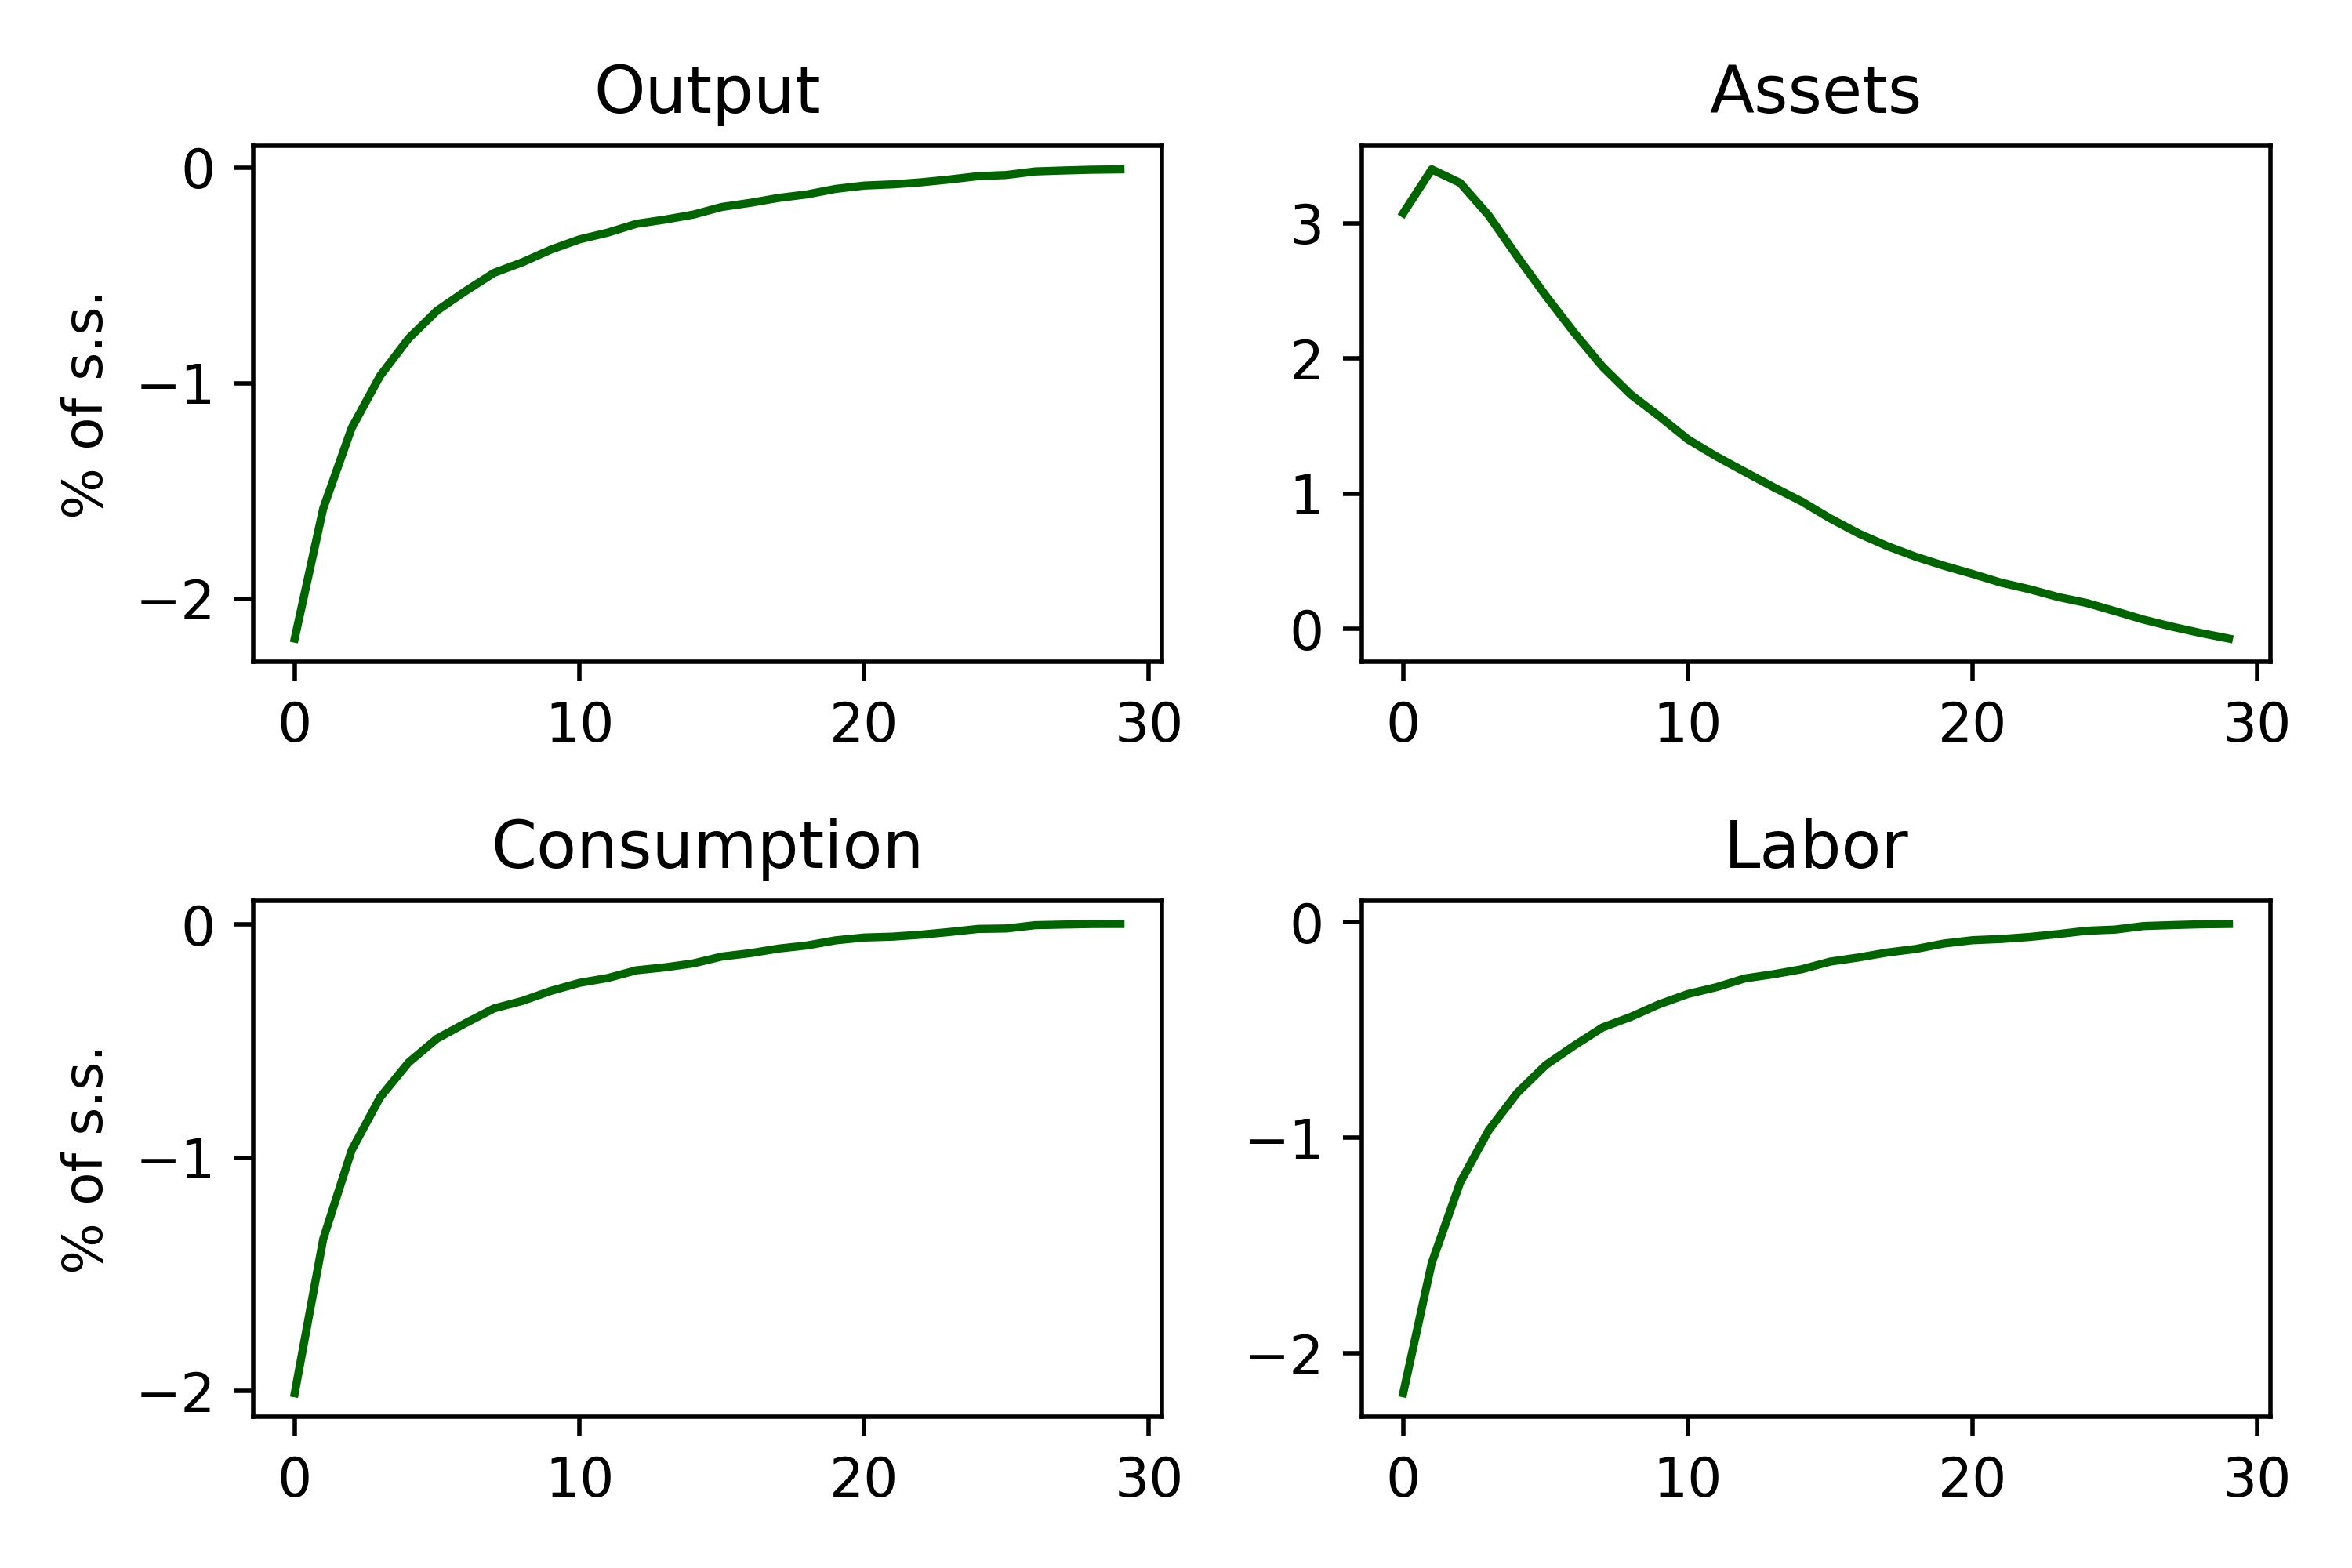
\includegraphics[scale=.35]{\FigDir/GIPRM2}
  \end{subfigure}
  \begin{subfigure}{}
    \centering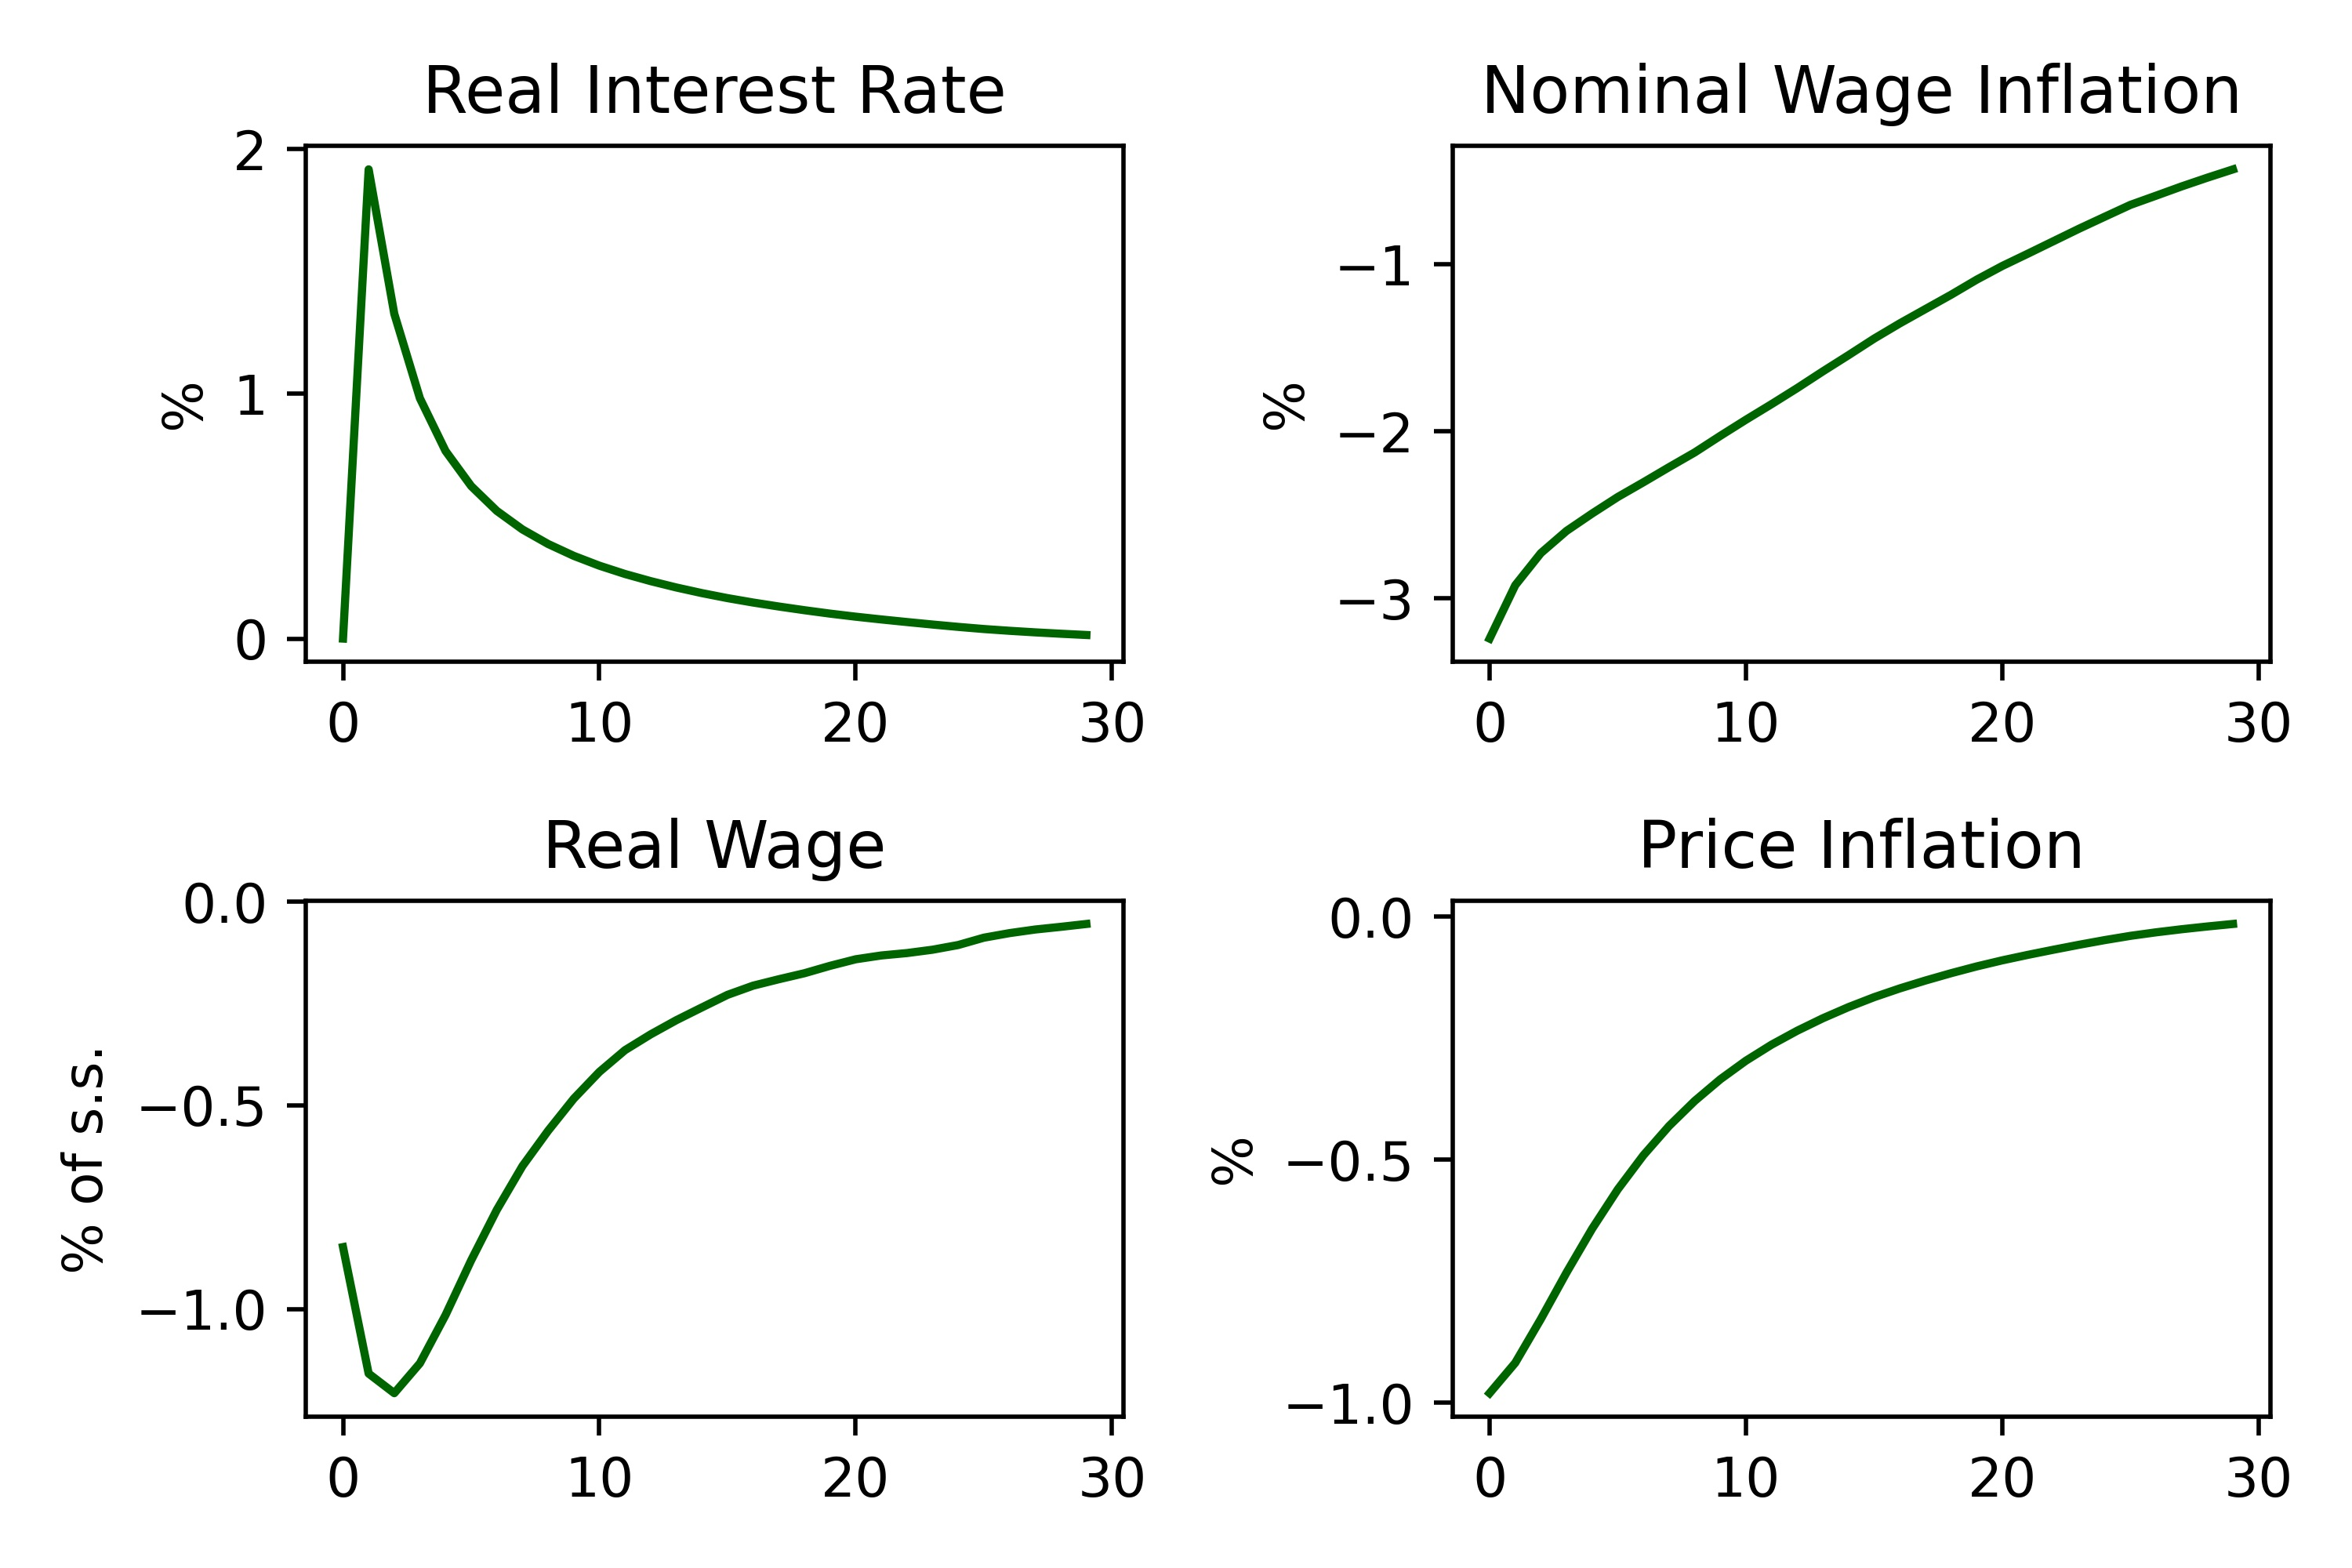
\includegraphics[scale=.35]{\FigDir/GIPRM1}
    \caption{ Impulse Response to One Percent Increase in Nominal Rate}
  \end{subfigure}
\end{figure}


\hypertarget{Productivity Shock}{}
\subsection{Productivity Shock}


The impulse responses to the productivity shock can be found in figure 2. The productivity shock is a 1 percent increase in $Z_{t}$ following an AR(1) with a coefficient of .9. The rise in productivity raises both output and firm markups, inducing downward pressure on prices which inturn induces downward pressure on nominal wages. However, given the goods market must clear, consumption must rise causing upward pressure on the nominal wage since the economy marginal rate of substitution is a function of the average marginal utility of consumption. The net effect will see nominal wages rise leading to upward pressure on prices. The net effect of all these different pressures will see the real wage rise and therefore amplify the consumption response signficantly due to the large aggregate MPC in the model. In addition, to the fixed nominal interest rate, inflation will see the real interest rate fall further amplifying consumption. This amplification of consumption will lead to rises in output and labor due to upward pressure on labor demand.

\begin{figure}{Impulse Responses to a Productivity Shock}
  \begin{subfigure}{}
    \centering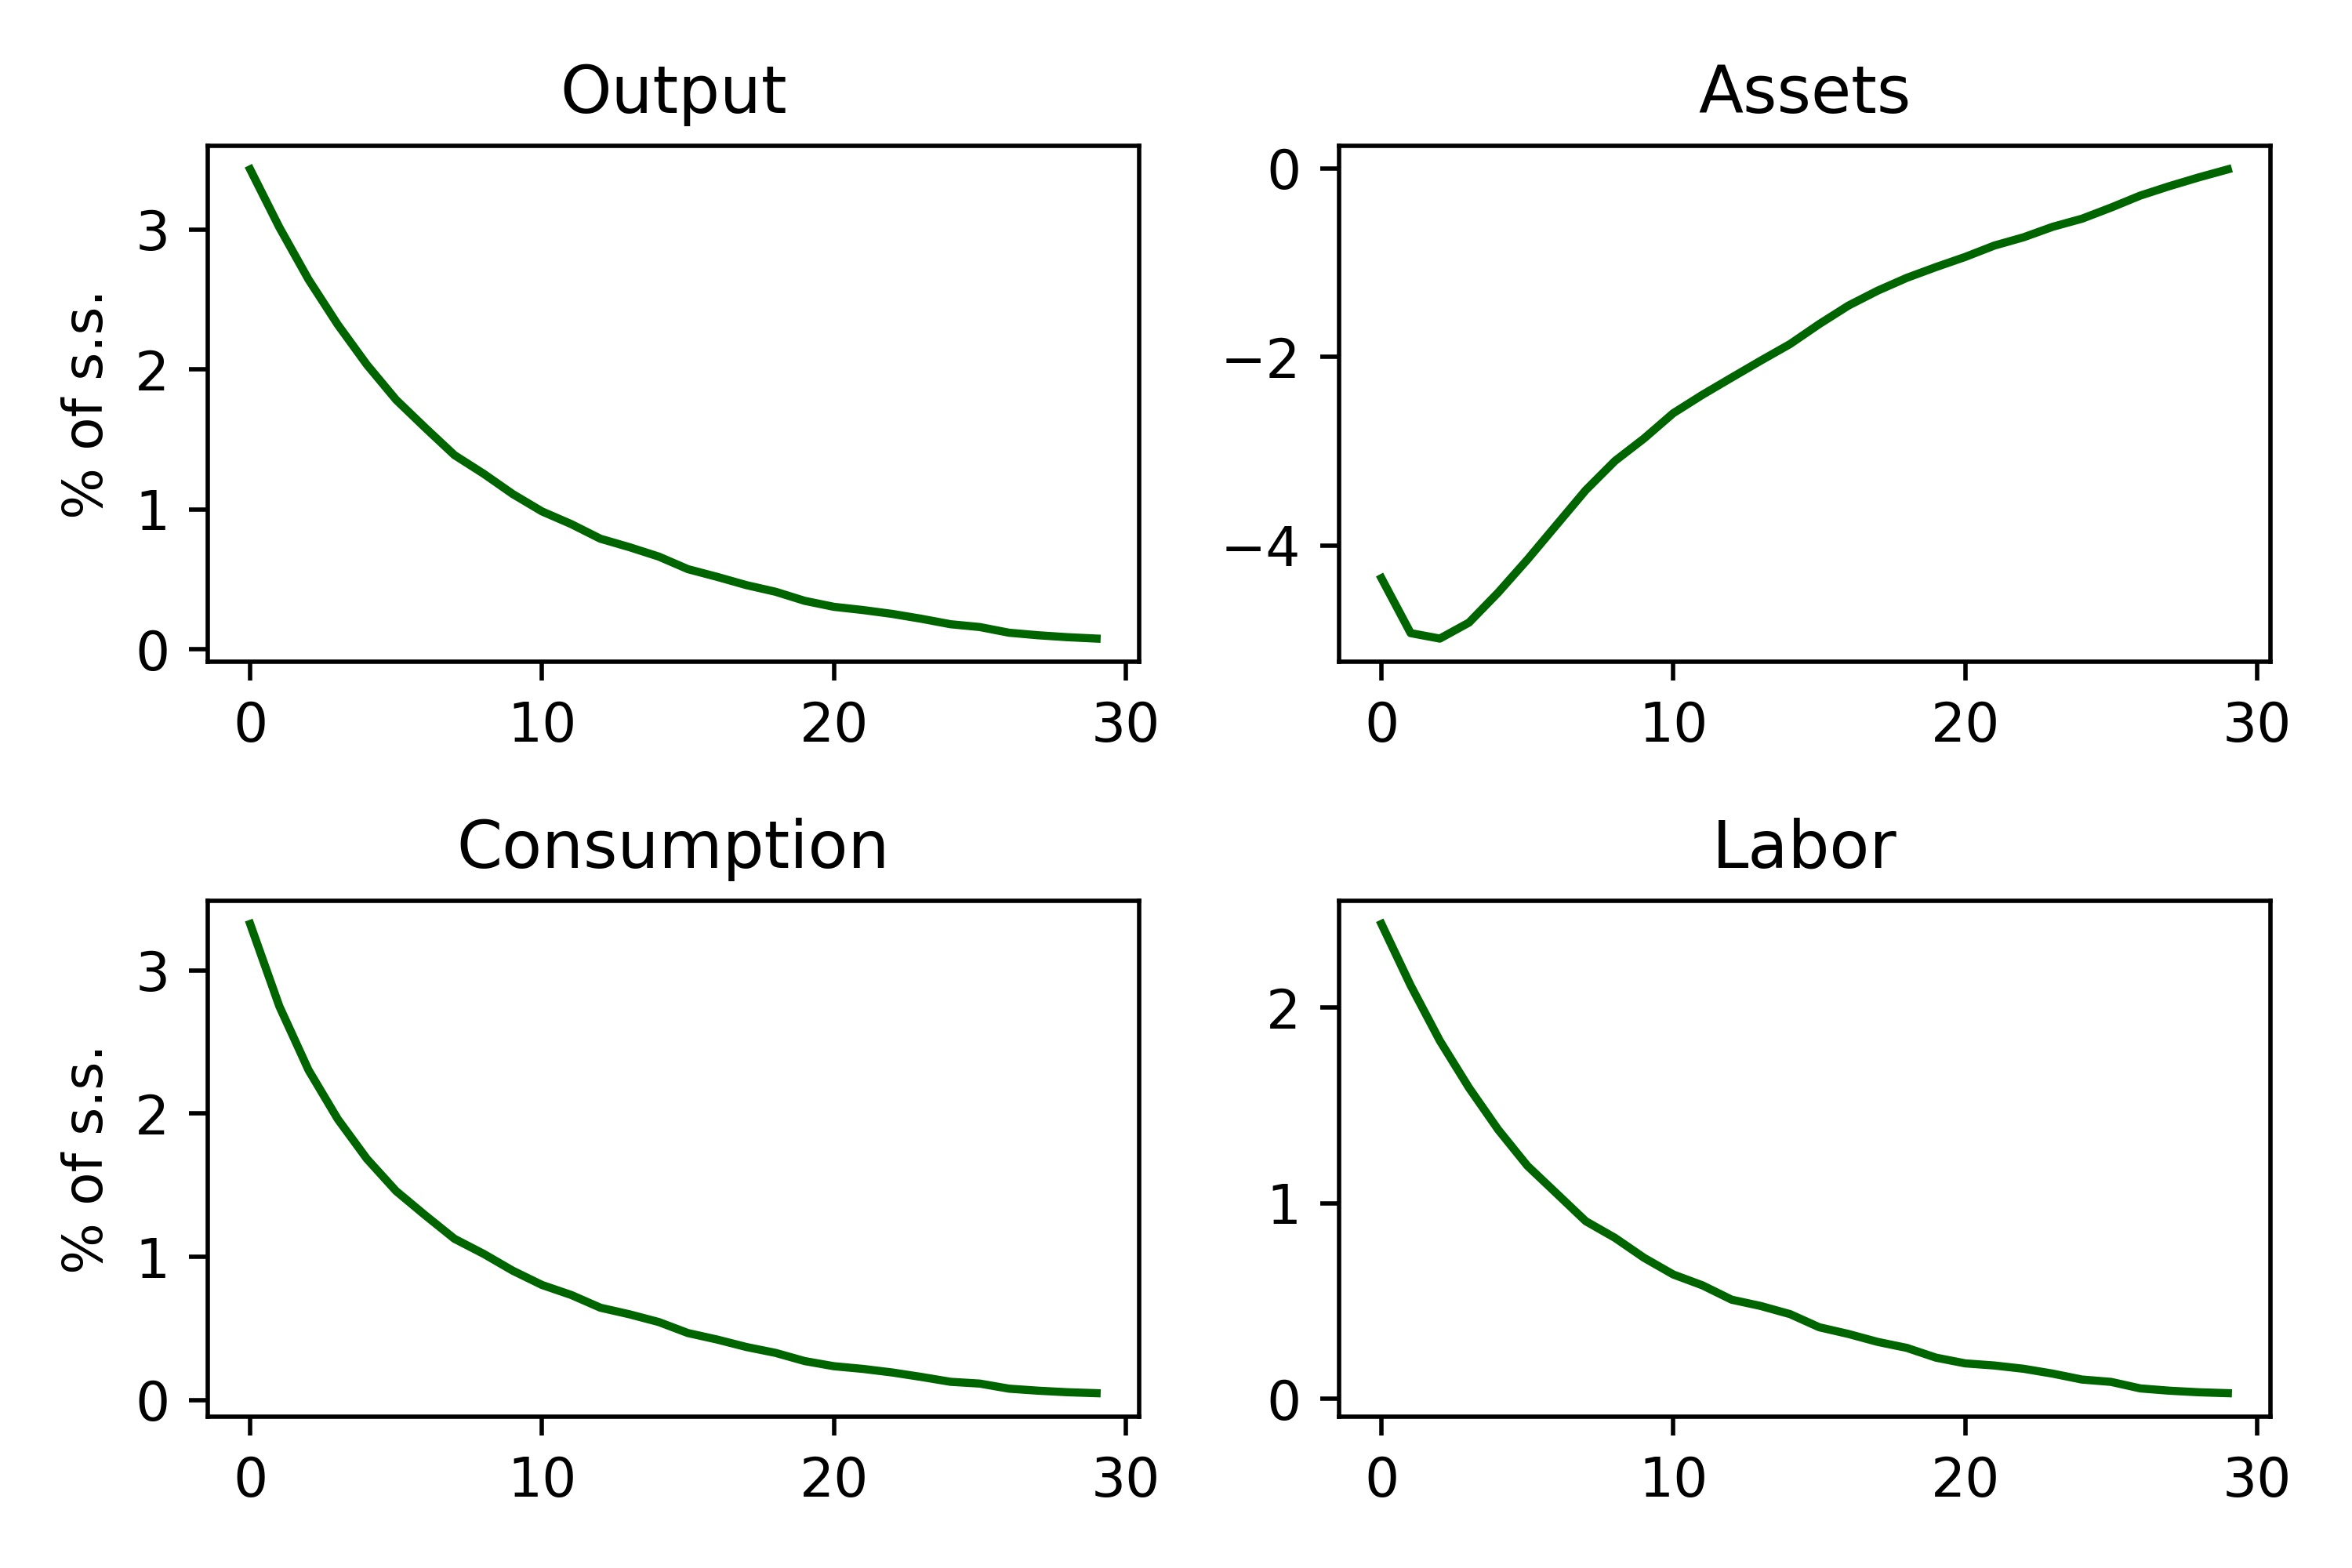
\includegraphics[scale=.35]{\FigDir/GIPRZ2}
  \end{subfigure}
  \begin{subfigure}{}
    \centering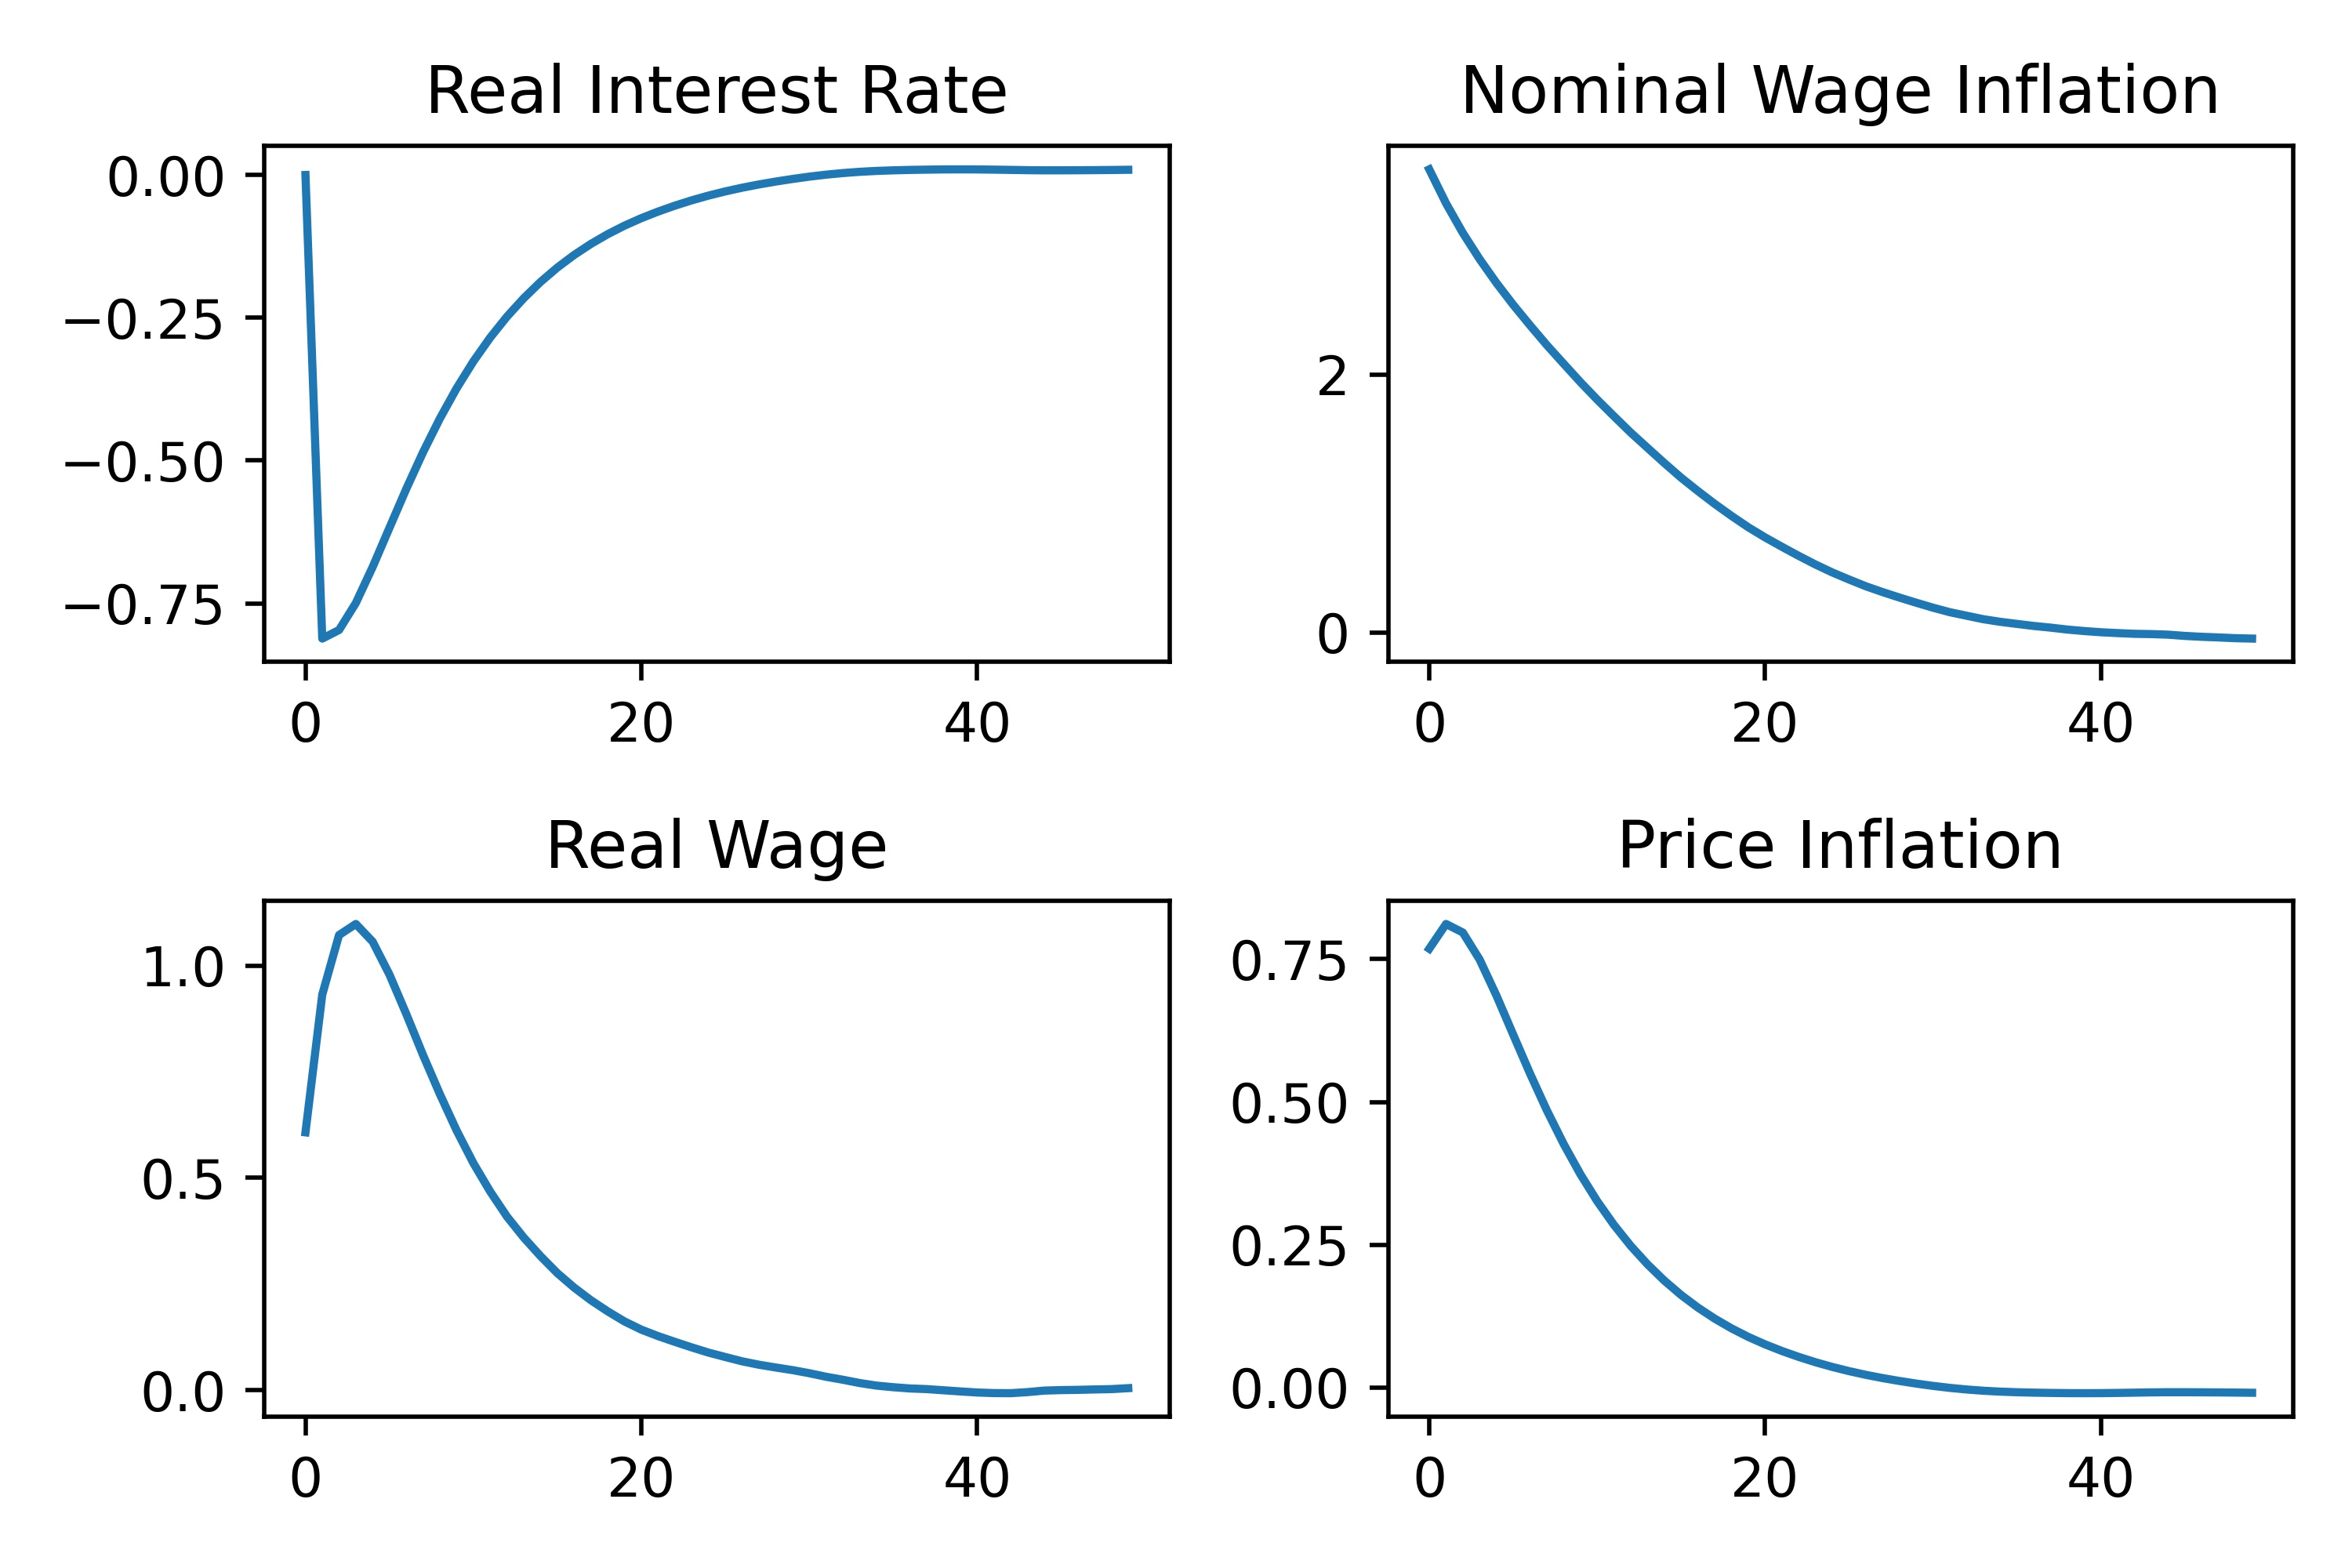
\includegraphics[scale=.35]{\FigDir/GIPRZ1}
    \caption{ Impulse Response to One Percent Increase in $Z_{t}$}
  \end{subfigure}
\end{figure}



\hypertarget{Issues and Extensions}{}
\section{Issues and Extensions}

The most prominent issue I have encountered thus far is determining whether the impulse responses are accurate in regards to the specification of the model. Producing the impulses responses is an exercise in linear algebra and the computation of jacobians. Because the jacobians were constructed without automatic differentiation, the accuracy of the impulse responses produced is uncertain as the smallest algebraic mistake may render them incorrect. Despite this uncertainty, the impulse responses of the model do mirror the responses produced from dynare under certain calibrations.  In particular, as long as prices are calibrated to be slightly stickier than wages, the impulse responses from a monetary policy shock behave in exactly the same manner as those produced from dynare. In addition, the impulse responses from a productivity shock seem essentially no different to those produced from dynare. The only issue is whenever wages are calibrated to be stickier than prices. When wages are stickier than prices,  to be specific, if the parameter for wage stickiness is set to .85 and the that of price stickiness to .8, the impulse responses to a monetary contraction are quantitatively the same as those seen in section 5 except they all invert across the x axis. That is, with the rise in the nominal rate, the results see a rise in consumption, output, labor, inflation and the real wage. This is much cause for concern regarding the accuracy of the code that produces the impulse responses as they do not survive under calibrations where wages are stickier than prices. It is possible, however, that these inverted responses may be accurate to the model due to the strong responsiveness of consumption present in the model. For instance, when the inverse frish elasticity is set to a large value (from v =2 to v=7) rendering labor to be significantly less sensitive to changes in wages, the impulse responses do not invert anymore ( consumption, output, labor, real wages all fall after a rise in the nominal rate). This is evidence that perhaps the consumption response is so strong that the slightest change in calibration could lead to large amplification effects that can invert the impulse response. My current hypothesis is that when prices are slightly more flexible than wages, the real wage may perhaps rise as since an increase in the nominal rate induces downward pressure on both prices and wages and if the fall in prices is larger than the fall in wages, the real wage may rise inducing a strong consumption response which amplifies and lead aggregate variables such as labor supply, and output to rise when the real rate rises. 
























%\providecommand{\figName}{GIPRM1}
%\providecommand{\figFile}{GIPRM1}
%\hypertarget{\figFile}{}
%\hypertarget{\figName}{}
%\begin{figure}[tbp]
%\centerline{\includegraphics[scale=.35]{\FigDir/\figFile}}
%\caption{Monetary Policy Shock}
%\label{fig:\figFile}
%\end{figure}


%%
%\renewcommand{\figFile}{GIPRM2}
%\hypertarget{\figFile}{}  
%\begin{figure}[tbp]
%\centerline{\includegraphics[scale=.35]{\FigDir/\figFile}}
%\caption{Monetary Policy Shock}
%\label{fig:\figFile}
%\end{figure}
%%


\clearpage\vfill\eject

\appendix

\centerline{\LARGE Appendices}\vspace{0.2in}




\hypertarget{Computational Details}{}
\section{Computational Details}

\hypertarget{Household Bellman Equation }{}
\subsection{Household Bellman Equation}

Household i's dynamic program is

$$ V(\pmb{\mathrm{m}}_{it},\pmb{\mathrm{p}}_{it})=\max_{ \{ \pmb{\mathrm{c}}_{it}\}} { \frac{\cLevBF_{i t}^{1-\rho}}{1 -\rho} - \varphi \pLevBF_{it} \frac{n_{it}^{1+v}}{1+v} + \beta_{i} \not D \mathrm{E}_{t}[V( \pmb{\mathrm{m}}_{it+1} , \pmb{\mathrm{p}}_{it+1})]}$$

subject to 

\begin{align*}
 \pmb{\mathrm{m}}_{i t} & = \pmb{\mathrm{z}}_{i t}  + (1+\mathit{r}^{a}_{t})\pmb{\mathrm{a}}_{i t-1} \\
 \pmb{\mathrm{c}}_{i t}  + \pmb{\mathrm{a}}_{i t} &= \pmb{\mathrm{z}}_{i t}  + (1+\mathit{r}^{a}_{t}) \pmb{\mathrm{a}}_{i t-1}   \\
\pmb{\mathrm{a}}_{it} &\geq 0 
\end{align*} \\ \\

This can be normalized to \\


$$ V(m_{it}) = \max_{\{c_{it}\}} {  \frac{c_{i t}^{1-\rho}}{1 -\rho} - \varphi \frac{n_{it}^{1+v}}{1+v} + \beta_{i}\not D \mathrm{E}_{t}[\psi_{it+1}^{1-\rho} V(m_{it+1})]}$$

 subject to 
 
 \begin{align*}
m_{i t} &=  \xi_{it}  + (1+r^{a}_{t}) \frac{a_{i t-1}}{\psi_{it}} \\
 c_{i t}  + a_{i t} &= \xi_{it}  + (1+r^{a}_{t}) \frac{a_{i t-1}}{\psi_{it}} \\
 a_{it} &\geq 0 
 \end{align*}
 
 Here non boldface variables are normalized by permanent income $\mathit{p_{it}}$. 

e.g. $x_{it} = \frac{\mathbf{x_{it}}}{\pmb{\mathrm{p}}_{it}}$ \\

First order condition for consumption:

$$c_{it}^{-\rho} -  \beta_{i} \not D \mathrm{E}_{t}\left[ (1+r^{a}_{t+1})  \psi_{it+1}^{-\rho} V'(m_{it+1})\right] = 0$$ \\ 



%%Now let $v(m_{it}, c_{it}) = \frac{c_{i t}^{1-\rho}}{1 -\rho} - \varphi \frac{n_{it}^{1+v}}{1+v} + \beta_{i}\not D \mathrm{E}_{t}[\psi_{it+1}^{1-\rho} V(m_{it+1})] $ and let $c_{it}(m_{it})$ denote the solution to the original dynamic problem.  \\ 

%%Note $ \frac{ \partial v(m_{it},c_{it}(m_{it}))}{\partial m} =  \beta_{i}\not D \mathrm{E}_{t}[\psi_{it+1}^{1-\rho} V'(m_{it+1})] $ \\

%%Then $$ V(m_{it}) = v(m_{it}, c_{it}(m_{it})$$ 

%%$$ V'(m_{it}) = \frac{ \partial v(m_{it},c_{it}(m_{it}))}{\partial m}$$ 

%%Which leads to the envelope condition \\

%%$$V'(m_{it}) =  \beta_{i}\not D \mathrm{E}_{t}[\psi_{it+1}^{1-\rho} V'(m_{it+1})] $$




\hypertarget{Model as System}{}
\subsection{Model as System}

The model can be defined by the system of equations below. The solution of the model must see this system be equal to a vector of zeros for periods $t =0, 1, 2, 3, ...$. The system is defined over the sequence space of all endogenous variables $\mathbf{U}$  and exogenous variables $\mathbf{Z}$ of the model.

$$
H_{t}(\mathbf{U},\mathbf{Z})= \begin{pmatrix} 
 Y_{t} - Z_{t}N_{t} \\ \\ 
B_{t-1} - q^{b}_{t}B_{t} + u\mho + G - \tau w_{t} N_{t} \\ \\  
i_{t} - r^{*} - \phi \pi^{p}_{t} -\phi_{y}(Y_{t}-Y_{ss}) - v_{t} \\ \\
\pi_{t}^{p} -\frac{\pi^{p}_{t+1}}{1+r^{*}} + \lambda(\mu_{t}^{p} -\mu_{p})  \\ \\
 \pi_{t}^{w} -\not D \pi_{t+1}^{w} -(\frac{1-\lambda_{w}}{\lambda_{w}}) (1- \not D \lambda_{w}) (\mu^{w} -\mu_{t}^{w}) \\ \\
    1+r_{t} - \frac{1 + i_{t}}{1+ \pi^{p}_{t+1}}\\ \\
 1+r_{t+1}^{a} - \frac{q_{t+1}^{s} +D_{t+1}}{q_{t}^{s}} \\ \\
 r_{t} - r_{t+1}^{a} \\ \\
 \frac{w_{t}}{w_{t-1}} - \frac{\Pi_{t}^{w}}{\Pi_{t}^{p}} \\ \\
 \mathcal{C}_{t}(\{r_{s}^{a} ,w_{s}, N_{s}\}_{s=0}^{s=T}) - Y_{t} + G \\ \\
 \end{pmatrix} = \begin{pmatrix} 0 \\ 0 \\. \\. \\. \\ 0\\ \end{pmatrix} , \quad t=0,1 ,2,3,....
$$ \\ \\
 

 
 where \\
 
$\mathcal{C}_{t}(\{r_{s}^{a} ,w_{s}, N_{s}\}_{s=0}^{s=T}) = \int_{0}^{1} \pLevBF_{it} c_{it}(m_{it})\, di $ \\
 
$c_{it}(m_{it})$ is the steady state normalized consumption policy for household $i$ in period t. \\ \\
 

 
 
 $\mathbf{U} = \left(Y_{t} , N_{t} ,  D_{t
 }, B_{t}, w_{t} , \pi_{t}^{p} ,\pi_{t}^{w}, r_{t} , r_{t+1}^{a}, i_{t} , q_{t}^{s},  q_{t}^{s} \right)_{t=0}^{t=T}$ \\ 

 
 $\mathbf{Z} = \left(Z_{t} ,v_{t}\right)_{t=0}^{t=T}$ \\
 
 \textbf{Note} the asset market clearing condition is not included in the system as the goods market clearing condition holds if and only if the asset market clearing condition holds. On the same note, the government budget constraint nor the equation for the stock price is included in the reduced system as they both bonds and its stock price appears in the asset clearing equation.  \\ \\
 
 
 
\hypertarget{Reduced System}{}
\subsubsection{Reduced System}
 
The previous system of a little more than a dozen endogenous variables can be reduced to a system of three endogenous variables. \\ 
 
Endogenous Variables are $ r_{t} , w_{t} ,N_{t}$ \\ 
 
Exogenous Variables are $ Z_{t}, v_{t}$ \\ 

The reduced system: \\ \\

\begin{eqnarray} 
H_{t}(\mathbf{U},\mathbf{Z})= \begin{pmatrix} 
\mathcal{H}_{t,1} \\ \\ 
\mathcal{H}_{t,2} \\ \\
\mathcal{H}_{t,3} \\ \\
 \end{pmatrix} = \begin{pmatrix} 0 \\ 0 \\ 0 \\ \end{pmatrix} , \quad  t = 0, 1, 2, ..., T 
 \end{eqnarray}
 
 where \\ 
 
 
 $\mathcal{H}_{t,1}  =\mathcal{C}_{t}\left( \left \{r^{a}_{s} , w_{s} , N_{s}  \right \}_{s=0}^{s=T} \right) - Z_{t} N_{t} + G\\ \\ $

$ \mathcal{H}_{t,2}  =log(w_{t}) - log(w_{t-1}) + \left( \frac{1 - \lambda_{w}}{\lambda_{w}}(1 - \not D \lambda_{w}) \sum_{k=0}^{\infty} \not D^{k} ( \mu_{t+k}^{w} - \mu^{w}) \right) - \left(  \lambda \sum_{k=0}^{\infty} \frac{1}{(1+r^{*})^{k}} ( \mu_{t+k}^{p} - \mu^{p})\right)\\ \\ $

$ \mathcal{H}_{t,3}  =  (1+r_{t}) \left(1+ -\lambda \sum_{k=1}^{\infty} \frac{1}{(1+r^{*})^{k}} ( \mu_{t+k}^{p} - \mu^{p}) \right) \\ \\
 - \left(1+r^{*}+ \phi \left(- \lambda \sum_{k=0}^{\infty} \frac{1}{(1+r^{*})^{k}} ( \mu_{t+k}^{p} - \mu^{p}) \right) +\phi_{y} \left(Z_{t} N_{t} - Y_{ss} \right) + v_{t}\right) \\ \\ $
 
$ \mu_{t}^{p} = log(\frac{1}{w_{t}}) + log(Z_{t})$ \\ 

$\mu_{t}^{w} = log(w_{t}) + log(1 - \tau_{t}) - mrs_{t} \\  $

$mrs_{t} = log \left(- \frac{\int_{0}^{1}   U_{n} \left(\cLevBF_{i t}, n_{i t} \right) \ d i  }{\int_{0}^{1} \pLevBF_{it} \theta_{it} U_{c} \left(\cLevBF_{i t}, n_{i t} \right) \  di } \right) = log \left(\frac{\int_{0}^{1} \varphi \pLevBF_{it} n_{it}^{v} \ d i  }{\int_{0}^{1} \pLevBF_{it}  \theta_{it} \cLevBF_{it}^{-\rho} \  di } \right) = log \left(\frac{\int_{0}^{1} \varphi \pLevBF_{it} \left(\frac{N_{t}}{1 - \mho} \right)^{v} \, d i  }{\int_{0}^{1} \pLevBF_{it}  \theta_{it} \cLevBF_{it}^{-\rho} \  di } \right)$ \\ 

$ = log \left( \varphi \left(\frac{N_{t}}{1 - \mho}\right) ^{v}\right) + log \left(\int_{0}^{1} \pLevBF_{it}  \,  di  \right) - log \left(\int_{0}^{1} \pLevBF_{it}  \theta_{it} \cLevBF_{it}^{-\rho} \  di  \right) $ \\ \\
 
 and the arguments of the function $H_{t}$ are \\
 
$\mathbf{U} = (r_{0} , r_{1} , ...r_{T}, w_{0}, w_{1}, ..., w_{T}, N_{0}, N_{1},...,N_{T})$ \\ 

$ \mathbf{Z} = ( Z_{0}, Z_{1},... Z_{T}, v_{0},...,v_{T}) \\ \\ $ 




\hypertarget{Jacobian of System}{}
\subsection{Jacobian of System} 

\hypertarget{Implicit Function Theorem}{}
\subsubsection{Implicit Function Theorem} 

By applying the implicit function theorem to the reduced system, we can obtain the endogenous responses of the real interest rate, wage, and labor supply given some exogenous shock \\

$$d\mathbf{U} =  -{\mathbf{H}_{\mathbf{U}}}^{-1} \mathbf{H}_{\mathbf{Z}} d \mathbf{Z}$$ \\ 

where $d\mathbf{U}$ are the endogenous responses of the real interest rate, the real wage, and labor supply to an exogenous shock $d \mathbf{Z}$.

Specifically, notation is defined below\\


$$d\mathbf{U} =(dr_{0} , dr_{1} , ...dr_{T}, dw_{0}, dw_{1}, ..., dw_{T}, dN_{0}, dN_{1},...,dN_{T})$$

$$d \mathbf{Z} = ( dZ_{0}, dZ_{1},... dZ_{T}, dv_{0},...dv_{T}) $$ \\





 $$  \mathbf{H}_{\mathbf{U}}= \begin{pmatrix} 
H_{\mathbf{U}, 1} \\ \\ 
H_{\mathbf{U}, 2}  \\ \\
H_{\mathbf{U}, 3} \\ \\
 \end{pmatrix} \quad \quad \mathbf{H}_{\mathbf{Z}}= \begin{pmatrix} 
H_{\mathbf{Z}, 1} \\ \\ 
H_{\mathbf{Z}, 2}  \\ \\
H_{\mathbf{Z}, 3} \\ \\
 \end{pmatrix}$$ \\ \\
 
 
 $$ H_{\mathbf{U}, i}= \begin{pmatrix} 
\frac{ \partial \mathcal{H}_{0,i}}{\partial r_{0}}  & ... & \frac{ \partial \mathcal{H}_{0,i}}{\partial r_{T}} & \frac{ \partial \mathcal{H}_{0,i}}{\partial w_{0}} & ... & \frac{ \partial \mathcal{H}_{0,i}}{\partial w_{T}} & \frac{ \partial \mathcal{H}_{0,i}}{\partial N_{0}} & ... &\frac{ \partial \mathcal{H}_{0,i}}{\partial N_{T}} \\ \\ 
\frac{ \partial \mathcal{H}_{1,i}}{\partial r_{0}}  & ... & \frac{ \partial \mathcal{H}_{1,i}}{\partial r_{T}} & \frac{ \partial \mathcal{H}_{1,i}}{\partial w_{0}} & ... & \frac{ \partial \mathcal{H}_{1,i}}{\partial w_{T}} & \frac{ \partial \mathcal{H}_{1,i}}{\partial N_{0}} & ... &\frac{ \partial \mathcal{H}_{1,i}}{\partial N_{T}}  \\ \\
.   \\ \\ \\ 
. \\ \\ \\
. \\ \\ \\
\frac{ \partial \mathcal{H}_{T,i}}{\partial r_{0}}  & ... & \frac{ \partial \mathcal{H}_{T,i}}{\partial r_{T}} & \frac{ \partial \mathcal{H}_{T,i}}{\partial w_{0}} & ... & \frac{ \partial \mathcal{H}_{T,i}}{\partial w_{T}} & \frac{ \partial \mathcal{H}_{T,i}}{\partial N_{0}} & ... &\frac{ \partial \mathcal{H}_{T,i}}{\partial N_{T}} \\ \\
 \end{pmatrix} $$ \\
 
  $$ H_{\mathbf{Z}, t}= \begin{pmatrix} 
\frac{ \partial \mathcal{H}_{0,i}}{\partial Z_{0}}  & ... & \frac{ \partial \mathcal{H}_{0,i}}{\partial Z_{T}} & \frac{ \partial \mathcal{H}_{0,i}}{\partial v_{0}} & ... & \frac{ \partial \mathcal{H}_{0,i}}{\partial v_{T}} \\ \\ 
\frac{ \partial \mathcal{H}_{1,i}}{\partial Z_{0}}  & ... & \frac{ \partial \mathcal{H}_{1,i}}{\partial Z_{T}} & \frac{ \partial \mathcal{H}_{1,i}}{\partial v_{0}} & ... & \frac{ \partial \mathcal{H}_{1,i}}{\partial v_{T}} \\ \\
. \\ \\ \\ 
. \\ \\ \\
. \\ \\ \\
\frac{ \partial \mathcal{H}_{T,i}}{\partial Z_{0}}  & ... & \frac{ \partial \mathcal{H}_{T,i}}{\partial Z_{T}} & \frac{ \partial \mathcal{H}_{T,i}}{\partial v_{0}} & ... & \frac{ \partial \mathcal{H}_{T,i}}{\partial v_{T}}  \\ \\
 \end{pmatrix} $$ \\ \\
 
 
\textbf{ Or equivalently}

 $$  \mathbf{H}_{\mathbf{U}}= \begin{pmatrix} 
H_{\mathbf{U}, 0} \\ \\ 
H_{\mathbf{U}, 1}  \\ \\
. \\ \\
. \\ \\
. \\ \\ 
H_{\mathbf{U}, T} \\ \\
 \end{pmatrix} \quad \quad \mathbf{H}_{\mathbf{Z}}= \begin{pmatrix} 
H_{\mathbf{Z}, 0} \\ \\ 
H_{\mathbf{Z}, 1}  \\ \\
. \\ \\
. \\ \\
. \\ \\ 
H_{\mathbf{Z}, T} \\ \\
 \end{pmatrix}$$ \\ \\
 
 
 
$$ H_{\mathbf{U}, t}= \begin{pmatrix} 
\frac{ \partial \mathcal{H}_{t,1}}{\partial r_{0}}  & ... & \frac{ \partial \mathcal{H}_{t,1}}{\partial r_{T}} & \frac{ \partial \mathcal{H}_{t,1}}{\partial w_{0}} & ... & \frac{ \partial \mathcal{H}_{t,1}}{\partial w_{T}} & \frac{ \partial \mathcal{H}_{t,1}}{\partial N_{0}} & ... &\frac{ \partial \mathcal{H}_{t,1}}{\partial N_{T}} \\ \\ 
\frac{ \partial \mathcal{H}_{t,2}}{\partial r_{0}}  & ... & \frac{ \partial \mathcal{H}_{t,2}}{\partial r_{T}} & \frac{ \partial \mathcal{H}_{t,2}}{\partial w_{0}} & ... & \frac{ \partial \mathcal{H}_{t,2}}{\partial w_{T}} & \frac{ \partial \mathcal{H}_{t,2}}{\partial N_{0}} & ... &\frac{ \partial \mathcal{H}_{t,2}}{\partial N_{T}}  \\ \\
\frac{ \partial \mathcal{H}_{t,3}}{\partial r_{0}}  & ... & \frac{ \partial \mathcal{H}_{t,3}}{\partial r_{T}} & \frac{ \partial \mathcal{H}_{t,3}}{\partial w_{0}} & ... & \frac{ \partial \mathcal{H}_{t,3}}{\partial w_{T}} & \frac{ \partial \mathcal{H}_{t,3}}{\partial N_{0}} & ... &\frac{ \partial \mathcal{H}_{t,3}}{\partial N_{T}} \\ \\
 \end{pmatrix} $$ \\
 
  $$ H_{\mathbf{Z}, t}= \begin{pmatrix} 
\frac{ \partial \mathcal{H}_{t,1}}{\partial Z_{0}}  & ... & \frac{ \partial \mathcal{H}_{t,1}}{\partial Z_{T}} & \frac{ \partial \mathcal{H}_{t,1}}{\partial v_{0}} & ... & \frac{ \partial \mathcal{H}_{t,1}}{\partial v_{T}} \\ \\ 
\frac{ \partial \mathcal{H}_{t,2}}{\partial Z_{0}}  & ... & \frac{ \partial \mathcal{H}_{t,2}}{\partial Z_{T}} & \frac{ \partial \mathcal{H}_{t,2}}{\partial v_{0}} & ... & \frac{ \partial \mathcal{H}_{t,2}}{\partial v_{T}} \\ \\
\frac{ \partial \mathcal{H}_{t,3}}{\partial Z_{0}}  & ... & \frac{ \partial \mathcal{H}_{t,3}}{\partial Z_{T}} & \frac{ \partial \mathcal{H}_{t,3}}{\partial v_{0}} & ... & \frac{ \partial \mathcal{H}_{t,3}}{\partial v_{T}}  \\ \\
 \end{pmatrix} $$ \\ \\
 
 
 
 
\hypertarget{Obtaining All Other Responses}{}
\subsubsection{Obtaining All Other Responses} 

To obtain all other responses given the endogenous response $\mathbf{dU}$, we compute the jacobians of the endogenous variable with respect to the relevant endogenous variables that have already been solved for.  For example, to compute the response of consumption to some exogenous shock $d\mathbf{Z}$, we sum  the jacobians of consumption with respect to the real interest rate, the wage and labor supply 

$$ d\mathbf{C} = \mathcal{J}^{\mathcal{C} , r} d\mathbf{r} +\mathcal{J}^{\mathcal{C} , w} d\mathbf{w} +\mathcal{J}^{\mathcal{C} , N} d\mathbf{N} $$\\
 
 where $\mathcal{J}^{\mathcal{C} , w} $ is the jacobian of aggregate consumption  $\mathcal{C}_{t}(\{r_{s}^{a} ,w_{s}, N_{s}\}_{s=0}^{s=T}) $  with respect to the wage. \\
 
 To be clear , 
 
$$d\mathbf{w} =  ( dw_{1}, dw_{2}, . . . , dw_{T})' $$
 
 
 
 $$\mathcal{J}^{\mathcal{C} , w} =   \begin{pmatrix} 
\frac{ \partial \mathcal{C}_{0}(\{r_{s}^{a} ,w_{s}, N_{s}\}_{s=0}^{s=T})}{\partial w_{0}}  & \frac{ \partial \mathcal{C}_{0}(\{r_{s}^{a} ,w_{s}, N_{s}\}_{s=0}^{s=T})}{\partial w_{1}}&    ... & \frac{ \partial \mathcal{C}_{0}(\{r_{s}^{a} ,w_{s}, N_{s}\}_{s=0}^{s=T})}{\partial w_{T}} \\ \\ 
\frac{ \partial \mathcal{C}_{1}(\{r_{s}^{a} ,w_{s}, N_{s}\}_{s=0}^{s=T})}{\partial w_{0}}  &\frac{ \partial \mathcal{C}_{1}(\{r_{s}^{a} ,w_{s}, N_{s}\}_{s=0}^{s=T})}{\partial w_{1}}& ... & \frac{ \partial \mathcal{C}_{1}(\{r_{s}^{a} ,w_{s}, N_{s}\}_{s=0}^{s=T})}{\partial w_{T}} \\ \\
.  \\ \\
.  \\ \\
. \\ \\
\frac{ \partial \mathcal{C}_{T}(\{r_{s}^{a} ,w_{s}, N_{s}\}_{s=0}^{s=T})}{\partial w_{0}}  &\frac{ \partial \mathcal{C}_{T}(\{r_{s}^{a} ,w_{s}, N_{s}\}_{s=0}^{s=T})}{\partial w_{1}}& ... & \frac{ \partial \mathcal{C}_{T}(\{r_{s}^{a} ,w_{s}, N_{s}\}_{s=0}^{s=T})}{\partial w_{T}}  \\ \\
 \end{pmatrix} $$ \\
 
  
\hypertarget{Additional Derivations}{}
\section{Additional Derivations} 

An employed household's transitory income is \\

$$ \theta_{it}(1-\tau) \int_{0}^{1} \frac{W_{gt}}{P_{t}}n_{igt}\,dg$$

where $W_{gt}$ denotes the nominal wage for labor type $g$ and $P_{t}$ the price of the final good. \\ \\

Now noitce

$$ \theta_{it}(1-\tau) \int_{0}^{1} \frac{W_{gt}}{P_{t}}\frac{N_{gt}}{1-\mho}\,dg$$

$$ \theta_{it}(1-\tau) \int_{0}^{1} \frac{W_{gt}}{P_{t}}\frac{\left(\frac{W_{gt}}{W_{t}}\right)^{-\epsilon_{w}} N_{t}}{1-\mho}\,dg$$

$$ \theta_{it}(1-\tau) \frac{N_{t}}{(1-\mho) W_{t}^{-\epsilon_{w}}P_{t}} \int_{0}^{1}  \left(W_{gt}\right)^{1-\epsilon_{w}} \,dg $$

$$\theta_{it}(1-\tau) \frac{N_{t}}{(1-\mho) W_{t}^{-\epsilon_{w}}P_{t}} W_{t}^{1-\epsilon_{w}} $$

$$ \theta_{it}(1-\tau) \frac{W_{t}N_{t}}{(1-\mho)P_{t} }$$\\

Which leads to the expression in the paper \\

$$ \theta_{it}(1-\tau) \frac{w_{t}N_{t}}{(1-\mho)}$$

\bibliography{\econtexRoot/BufferStockTheory,economics}

Auclert et al 2020

Auclert et al 2021

Carroll 2006

CSTW(2017)

 Chetty(2012)

Reiter 2009

Simon (1956)

Theil (1957)






\end{document}
